\documentclass[12pt]{article}
\usepackage{amsmath}
\usepackage{float}
\usepackage{graphicx}
\usepackage{tabularx,ragged2e,booktabs,caption}
\usepackage{caption}
\usepackage{subcaption}
 \usepackage{slashed}
 \usepackage{multicol}
 \usepackage{flexisym}
 \usepackage{amsmath}
 \usepackage{amsfonts}
 \usepackage{amssymb}
 \usepackage{float}
 \usepackage{amsmath}
 \usepackage{multicol}
 
%\usepackage{lipsum}
\usepackage[margin=.6in,footskip=0.25in]{geometry}
\title{Dept project}
\author{Soumen}
\makeindex
\begin{document}

\begin{titlepage}
	\centering

	{\huge\bfseries  Performance of Belle II }
	\\	\vspace{4mm}
	{\huge\bfseries Silicon Vertex Detector in Phase2 }\\
	\vspace{2cm}
		{\huge\bfseries Soumen Halder }\\
		\vspace{2cm}
	
	
\includegraphics[width = 50mm]{belle2.png}
	
	
	\vfill
	
	\vfill		
	% Bottom of the page
	{\large \today\par}
\end{titlepage}
	\tableofcontents
	\pagebreak
% Start the document
    \section{Data Sample} Two Phase2 data sample is used in my analysis.
     \subsection{Bhabha Sample ($e^+ e^-\rightarrow e^+ e^-$)}
     \subsubsection{Location} \textbf{hlt\_bhabha} skim raw data used from KEKCC(/ghi/fs01/belle2/bdata/Data/release-02-00-01/\\DB00000425/prod00000005/e0003/4S/r*/all/raw/sub00/raw.physics.hlt\_bhabha*) 
     \subsubsection{Furthur selection cut}
     	
     	  \begin{itemize}
     	  	\item \# of tracks=2
     	  	
     	  	\item acollinearity$<10^{\circ}$
     	  	\item Momentum of each of two tracks $>$ 3GeV 
     	  	\item $|d_0|<2$ cm and $|z_0|<4$ cm		
     	  \end{itemize}
     
     \subsection{ Dimuon Sample ($e^+ e^-\rightarrow \mu^+ \mu^-$)}
     \subsubsection{Location}  \textbf{hlt\_mumu\_2trk} skim raw data used from KEKCC(/ghi/fs01/belle2/bdata/Data/release-02-00-01/\\DB00000425/prod00000005/e0003/4S/r*/all/raw/sub00/raw.physics.hlt\_mumu\_2trk*) 
     \subsubsection{Furthur selection cut}
     \begin{itemize}
     	\item \# of tracks=2
     	\item $35^{\circ}<\theta<125^{\circ}$
     	\item acollinearity$<10^{\circ}$
     	\item 0 GeV$<$EClenergy$<0.7$GeV
     	\item $|d_0|<2$ cm and $|z_0|<4$ cm		
     \end{itemize}
     \rule{\textwidth}{0.4pt}
     \pagebreak	
     
	\section{Hit Efficiency}
	\subsection{Definition}
	 Hit efficiency is probability of finding a hit in a SVD sensor  when we know the track pass through that sensor.
	 \subsection{Procedure} Efficiency is calculated  by fitting the track without hit of the layer we wish to find efficiency. Then  extrapolating the track to that sensor plane and 
	 then look for hit within $\pm$ 500 $\mu\rm{m}$ window from the position of extrapolation of the track. That is efficiency =$\frac{\rm{\# hits}}{\rm{\#tracks}}$. If there are multiple hits that hit is taken which is closest to track extrapolated position on sensor plane.
	 \subsubsection{Selection criteria} The selection criteria applied for choosing tracks are,
	 \begin{itemize}
	 	\item  hits associated to the track must contain
	 	\begin{itemize}
	 		\item[$=>$] at least one layer PXD hit
	 		\item[$=>$] at least one layer SVD hit
	 	\end{itemize}
	 	\item position of track extrapolated to sensor plane should lie within 20 strips inside from sensor edge
	 \end{itemize}
	 \subsubsection{Correction due to background cluster}
	 \begin{multicols}{2}
	 	 Due to background cluster the number of hits within $\pm$500$\mu \rm{m}$ window can be contributed by noise. For that we have to estimate the number of noisy hits($\rm{N}_{\rm{bkg}}$) within signal band. This is done by assuming that number of noisy cluster is uniform and from the sideband region [$\pm500 \mu \rm{m}$,$\pm1000 \mu \rm{m}$] we are estimating $\rm{N}_{\rm{bkg}}$. So corrected defination of efficiency is $$\text{Efficiency}=\frac{\text{N}-\text{N}_{\text{bkg}}}{\text{\# of tracks}}$$
	 	 Where N is total number of hits inside signal band.
	 	 	\begin{figure}[H]
	 	 		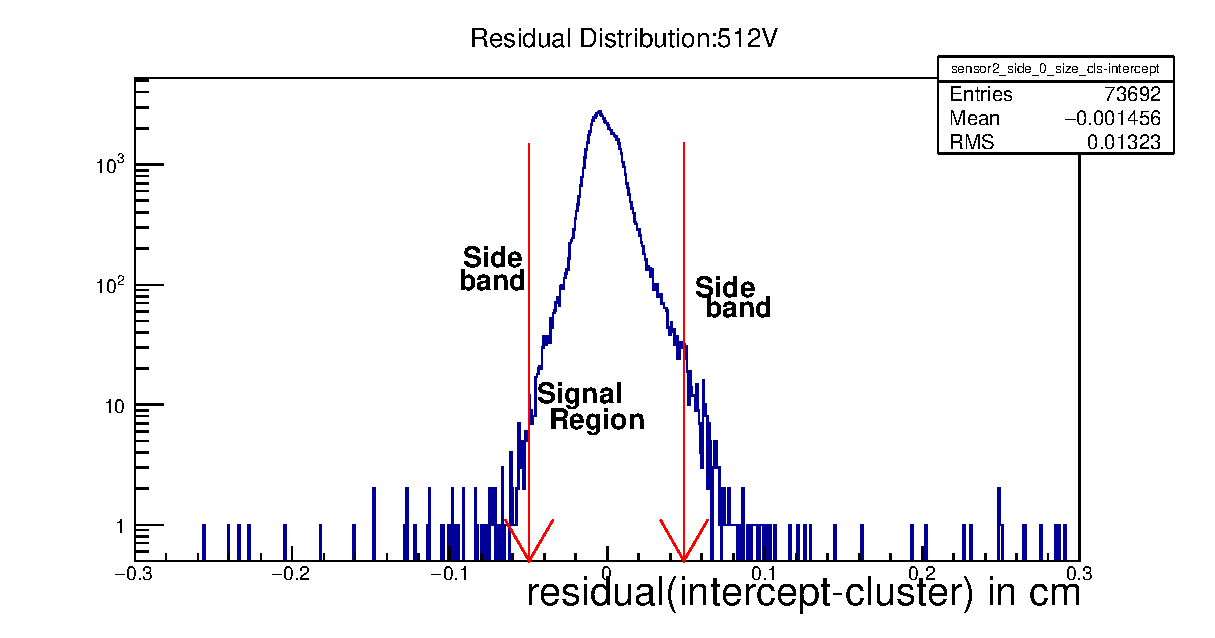
\includegraphics[width=.5\textwidth]{nbkg.eps}	
	 	 		\caption{Distribution of Residual(=position of track extralpolated position on sensor plane--position of hit). N is number of entry within signal band of this plot. $\text{N}_{\text{bkg}}$ is number of entry within [-0.1,-0.05] and [0.05,0.1] window}	
	 	 		\label{fig1}	
	 	 	\end{figure}
	 	\end{multicols}
	 
	\subsubsection{Error Calculation}
	    According to the definition of efficiency the \# of hits for a given number of tracks(n) is binomial distribution where probability(p) of having one hit for a given track is efficiency. So error on \# of hits = $\sqrt{np(1-p)}$.
	    So error on efficiency is $\frac{\sqrt{np(1-p)}}{n}$
	    $$\Delta\text{Efficiency}=\sqrt{\frac{\text{Efficiency}(1-\text{Efficiency})}{\text{\# of tracks}}}$$
	\begin{table}
		
		\begin{tabular}{|c|c|c|c||| c|c|c|}
			\hline
			Sensors	&	\multicolumn{3}{|c|}{Bhabha } &\multicolumn{3}{|c|}{Dimuon }\\ \cline{2-7}
			& U &Modified U&V & U&Modified U& V\\ \cline{1-7}
			311 	&99.08  $\pm$ 0.02 &                      &99.44  $\pm$  0.02  &  98.58  $\pm$  0.29&                      &99.59    $\pm$ 0.16  \\
			312 	&99.09  $\pm$ 0.02 &                      &99.09  $\pm$  0.02  &  98.81  $\pm$  0.13&                      &98.97    $\pm$ 0.12  \\ \hline
			
			411 	&                  &                      &99.31  $\pm$  0.02  &                    &                      &99.84    $\pm$ 0.16  \\
			412 	&80.53  $\pm$ 0.12 & 98.47 $\pm$ 0.04     &97.32  $\pm$  0.05  &  79.00  $\pm$  0.47&  98.40 $\pm$ 0.17    &97.30    $\pm$ 0.19  \\
			413 	&99.53  $\pm$ 0.02 &                      &99.51  $\pm$  0.02  &  99.31  $\pm$  0.69&                      &100.00   $\pm$ 0.00  \\ \hline
			
			511 	&                  &                      &97.81  $\pm$  0.06  &                    &                      &                        \\
			512	&84.50  $\pm$ 0.12 & 99.11$\pm$ 0.03      &97.90  $\pm$  0.05  &  84.59  $\pm$  0.65&  98.82  $\pm$ 0.22   &99.15    $\pm$ 0.17  \\
			513	&98.48  $\pm$ 0.04 &                      &95.69  $\pm$  0.06  &  98.25  $\pm$  0.20&                      &94.27    $\pm$ 0.35  \\
			514	&99.82  $\pm$ 0.02 &                      &99.50  $\pm$  0.03  &  100.00 $\pm$  0.00&                      &100.00   $\pm$ 0.00  \\ \hline
			
			611	&                  &                      &99.42  $\pm$  0.04  &                    &                      &                      \\
			612	&84.85  $\pm$ 0.13 & 99.46 $\pm$0.03      &97.37  $\pm$  0.06  &  86.43  $\pm$  0.99&  99.39  $\pm$0.25    &98.24    $\pm$ 0.38  \\
			613&82.85  $\pm$ 0.19 & 98.70 $\pm$0.06      &99.23  $\pm$  0.04  &  82.52  $\pm$  0.65&  98.77  $\pm$0.21    &99.25    $\pm$ 0.15  \\
			614&98.12  $\pm$ 0.04 &                      &98.71  $\pm$  0.04  &  98.15  $\pm$  0.32&                      &98.90    $\pm$ 0.25  \\
			615	&99.70  $\pm$ 0.04 &                      &99.17  $\pm$  0.06  &                     &                      &                    \\ \hline
		\end{tabular}
			\caption{This is the table summarizing efficiency of Bhabha($e^+ e^-\rightarrow e^+ e^-$) and Dimuon($e^+ e^-\rightarrow \mu^+ \mu^-$) sample for phase2 data. For 412U,512U,612U,613U sensors the efficiency is recalculated excluding the tracks which lies with 108$<$stripID$<$276. These region corresponds to that APV which was masked for most of the run in phase2  }		
			\label{tab1}	
    \end{table}
    \rule{\textwidth}{0.4pt}
	\pagebreak	
	
	\section{Hit Resolution and Residual plots} Here I am sowing the Residual plots, whose width can be used to find hit resolution, taking into account error associated to extrapolated track position on sensor plane. Some Residual plots has tail, some of then are shifted. That's why here I am showing the correlation of residual with cluster position. All the residual plot showing below is for Bhabha sample(having enough statistics) 
	\subsection{Layer3}
	\subsubsection{Sensor:1 U\_side}
	\begin{multicols}{3}
		
		\begin{figure}[H]
			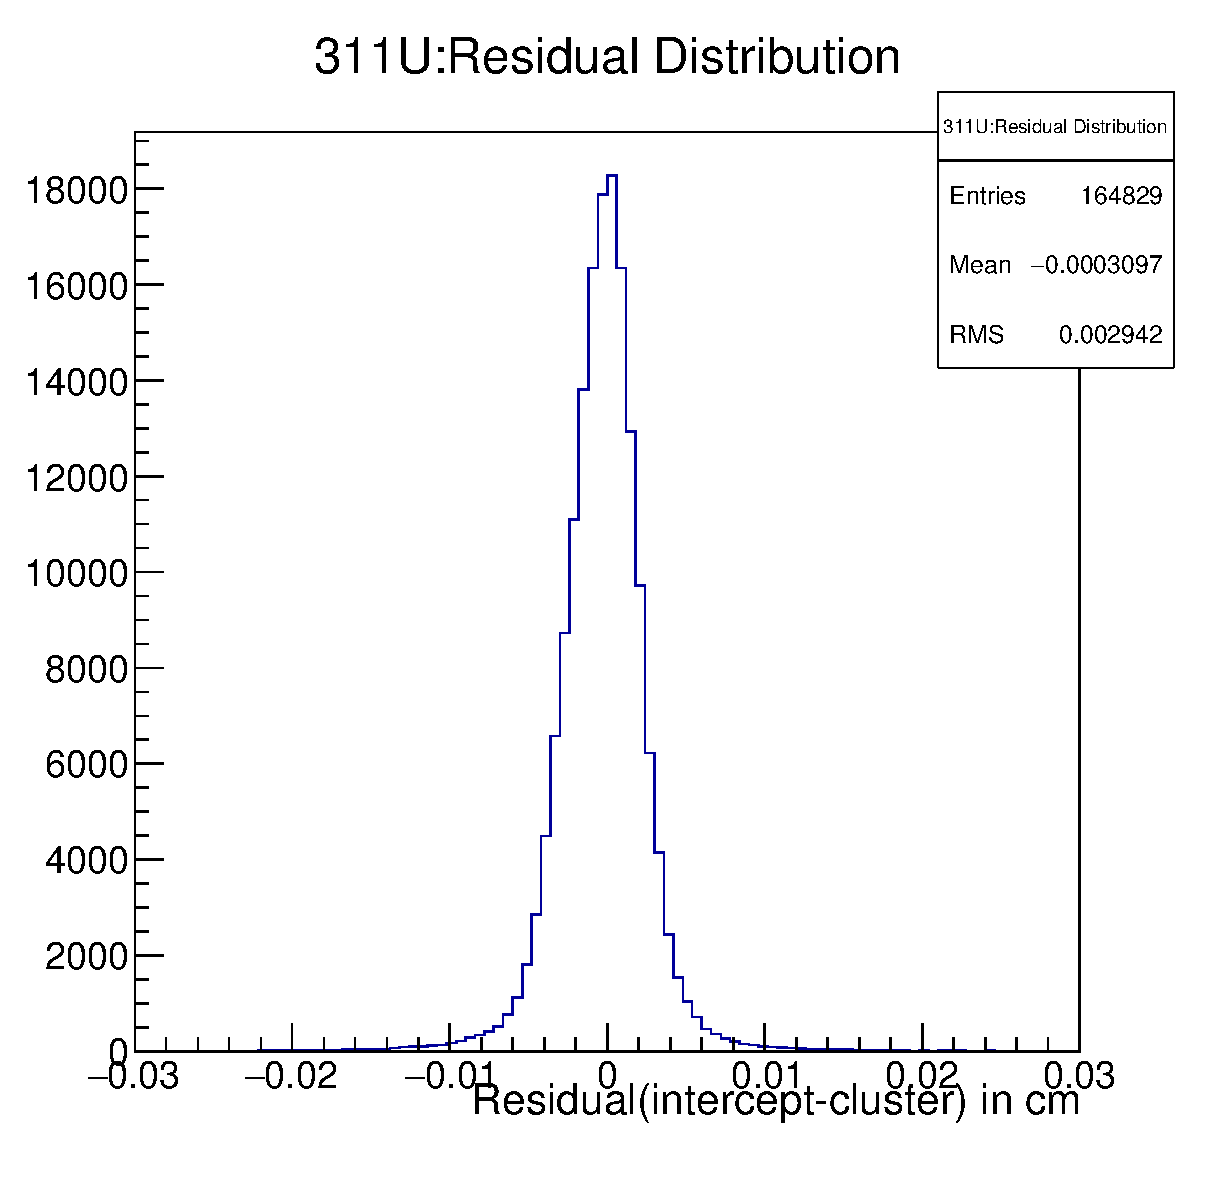
\includegraphics[width=.3\textwidth]{311U:residualplot.eps}	
			\caption{Residual distribution}	
			\label{fig1}	
		\end{figure}
		\begin{figure}[H]
			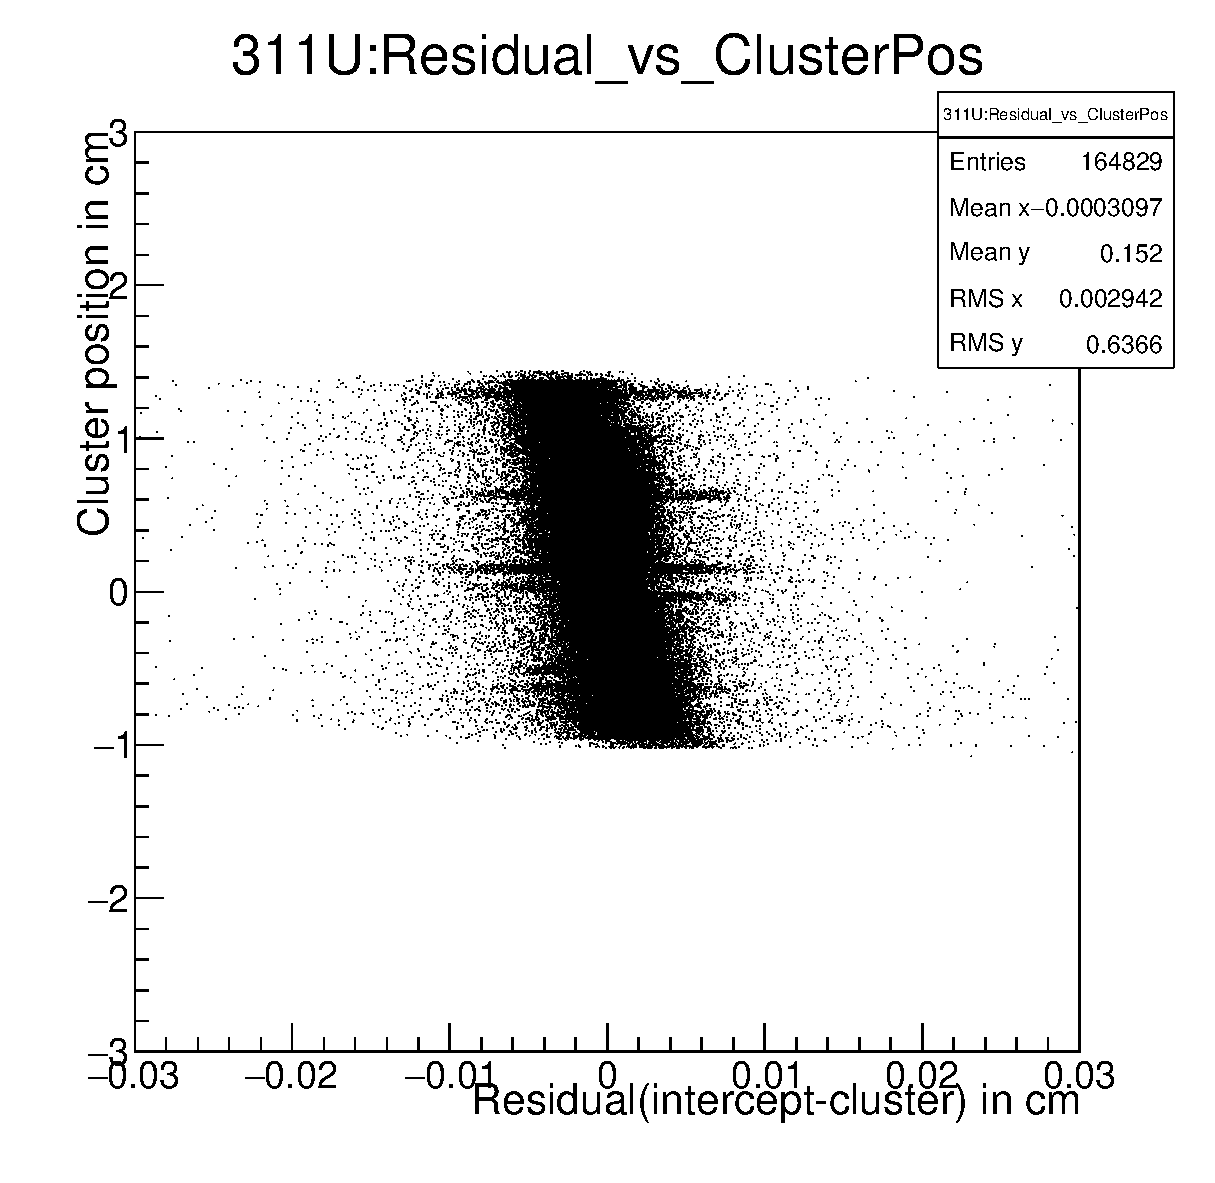
\includegraphics[width=.3\textwidth]{311U:residual_vs_clusterpos.eps}	
			\caption{Cluster position vs Residual}	
			\label{fig2}	
		\end{figure}
		\begin{figure}[H]
			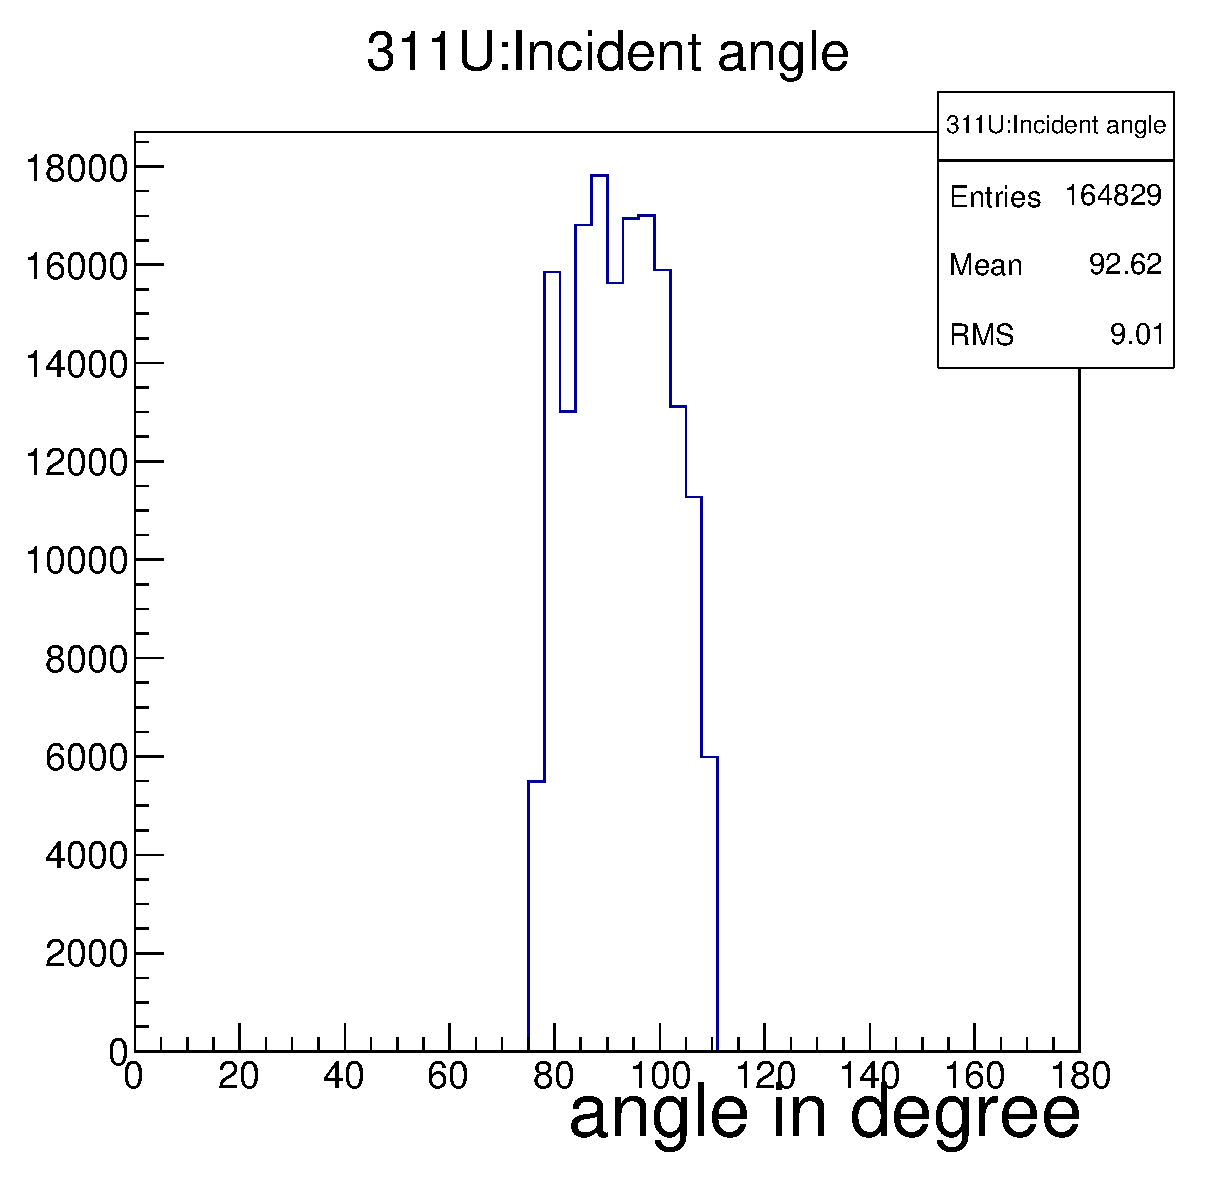
\includegraphics[width=.3\textwidth]{311U:incident_angle.eps}	
			\caption{Incident angle of the tracks}	
			\label{fig2}	
		\end{figure}
	\end{multicols}
	
		\begin{multicols}{4}
			
			\begin{figure}[H]
				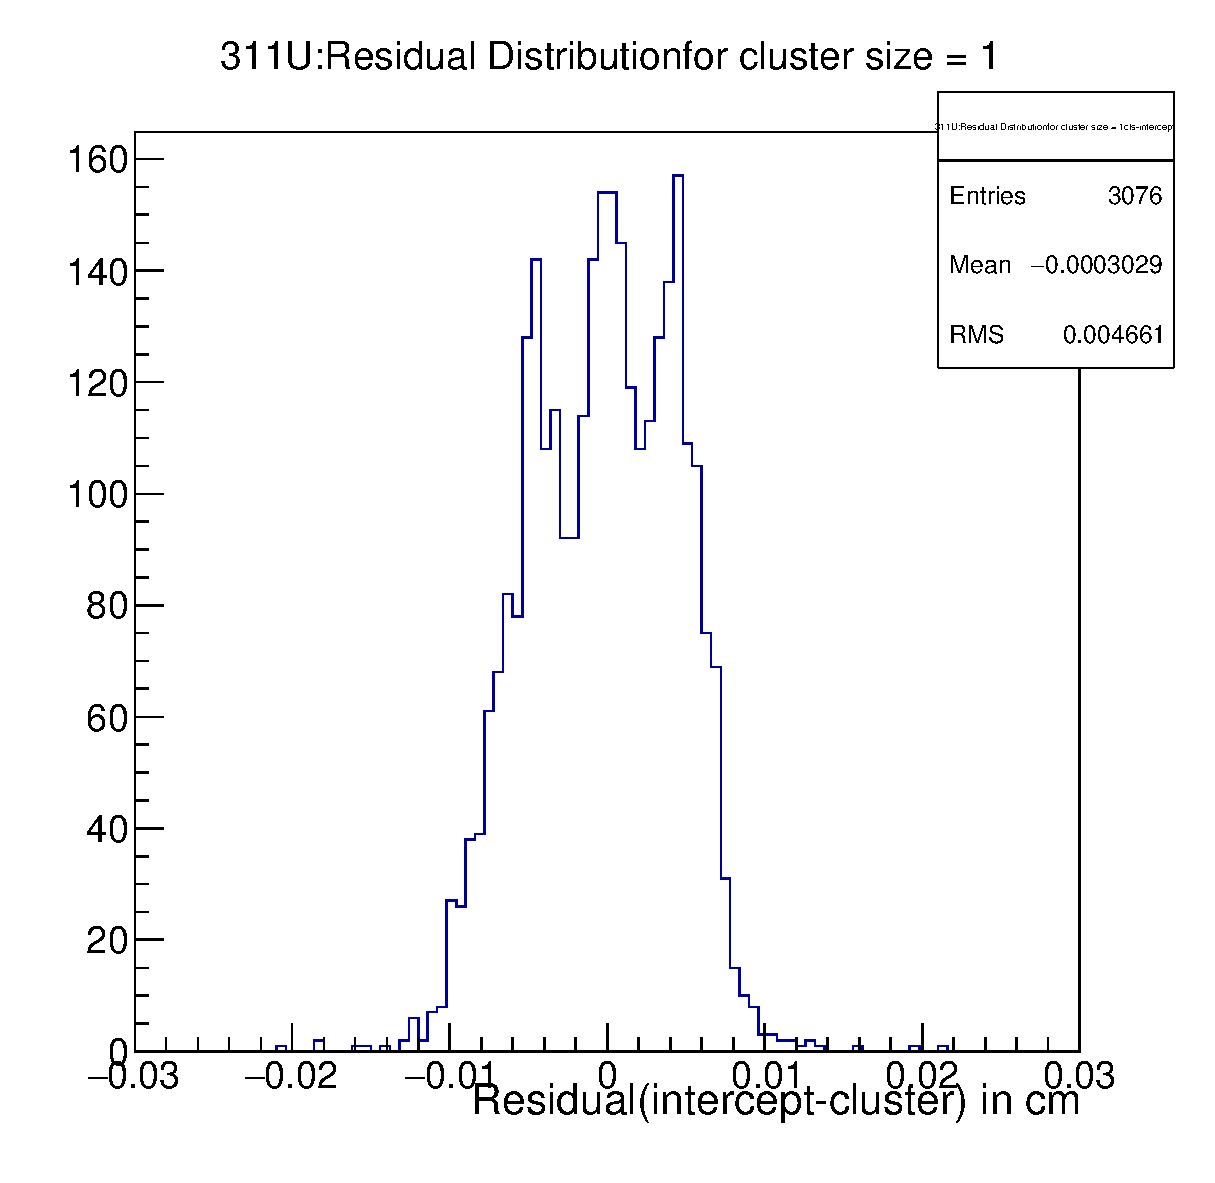
\includegraphics[width=.2\textwidth]{311U:clssize1.eps}	
				\caption{Residual distribution:Cluster size=1}	
				\label{fig1}	
			\end{figure}
			\begin{figure}[H]
				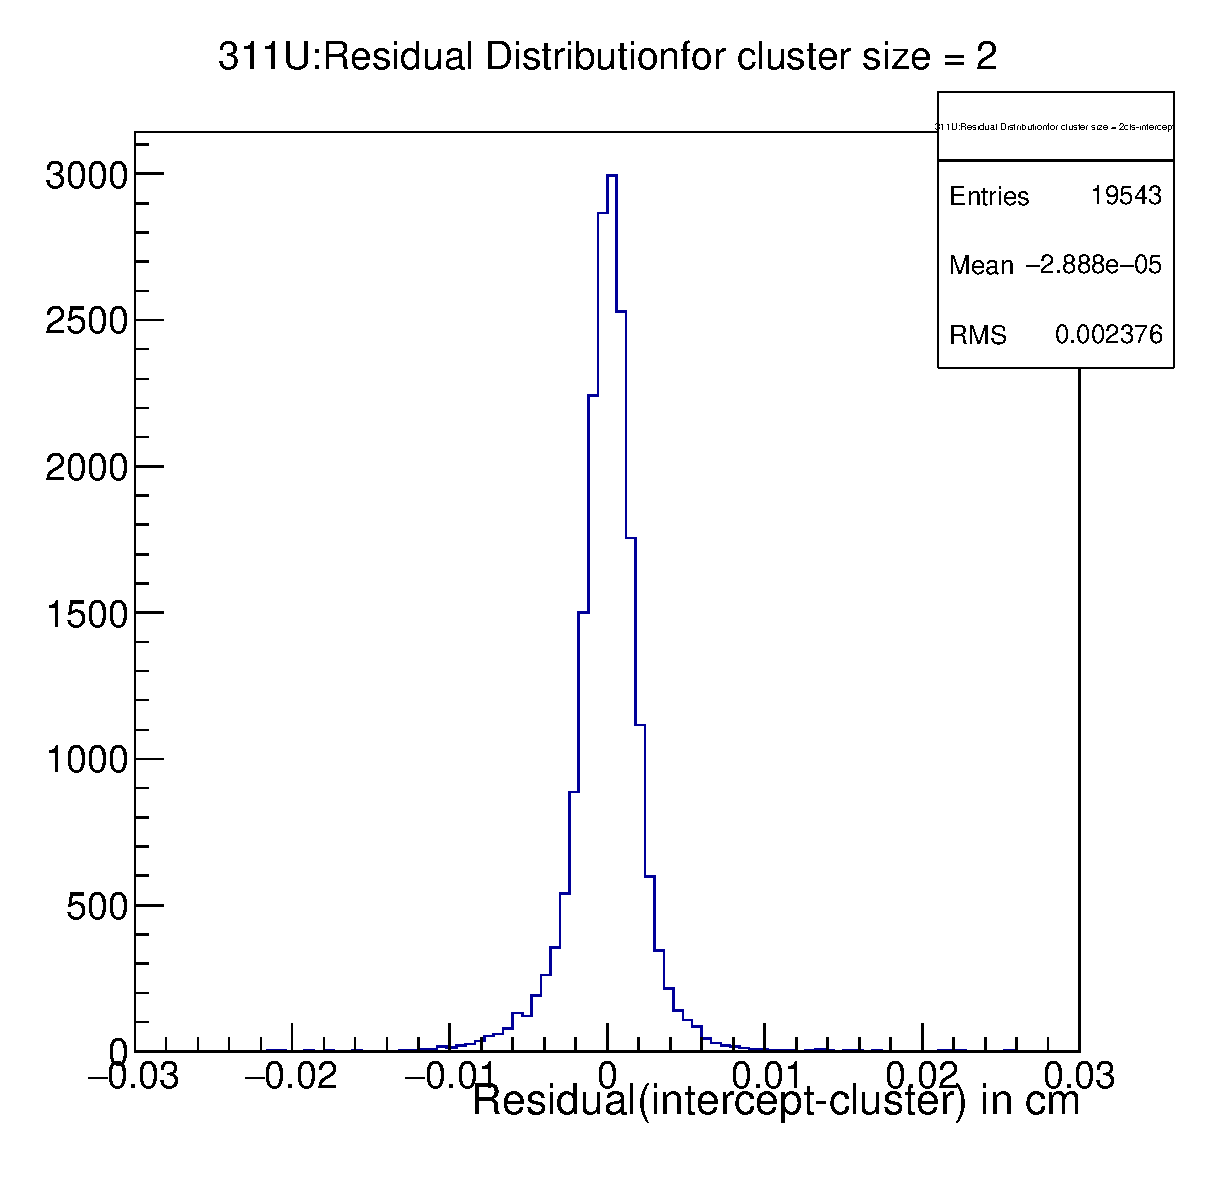
\includegraphics[width=.2\textwidth]{311U:clssize2.eps}	
				\caption{Residual distribution:Cluster size=2}	
				\label{fig2}	
			\end{figure}
				\begin{figure}[H]
					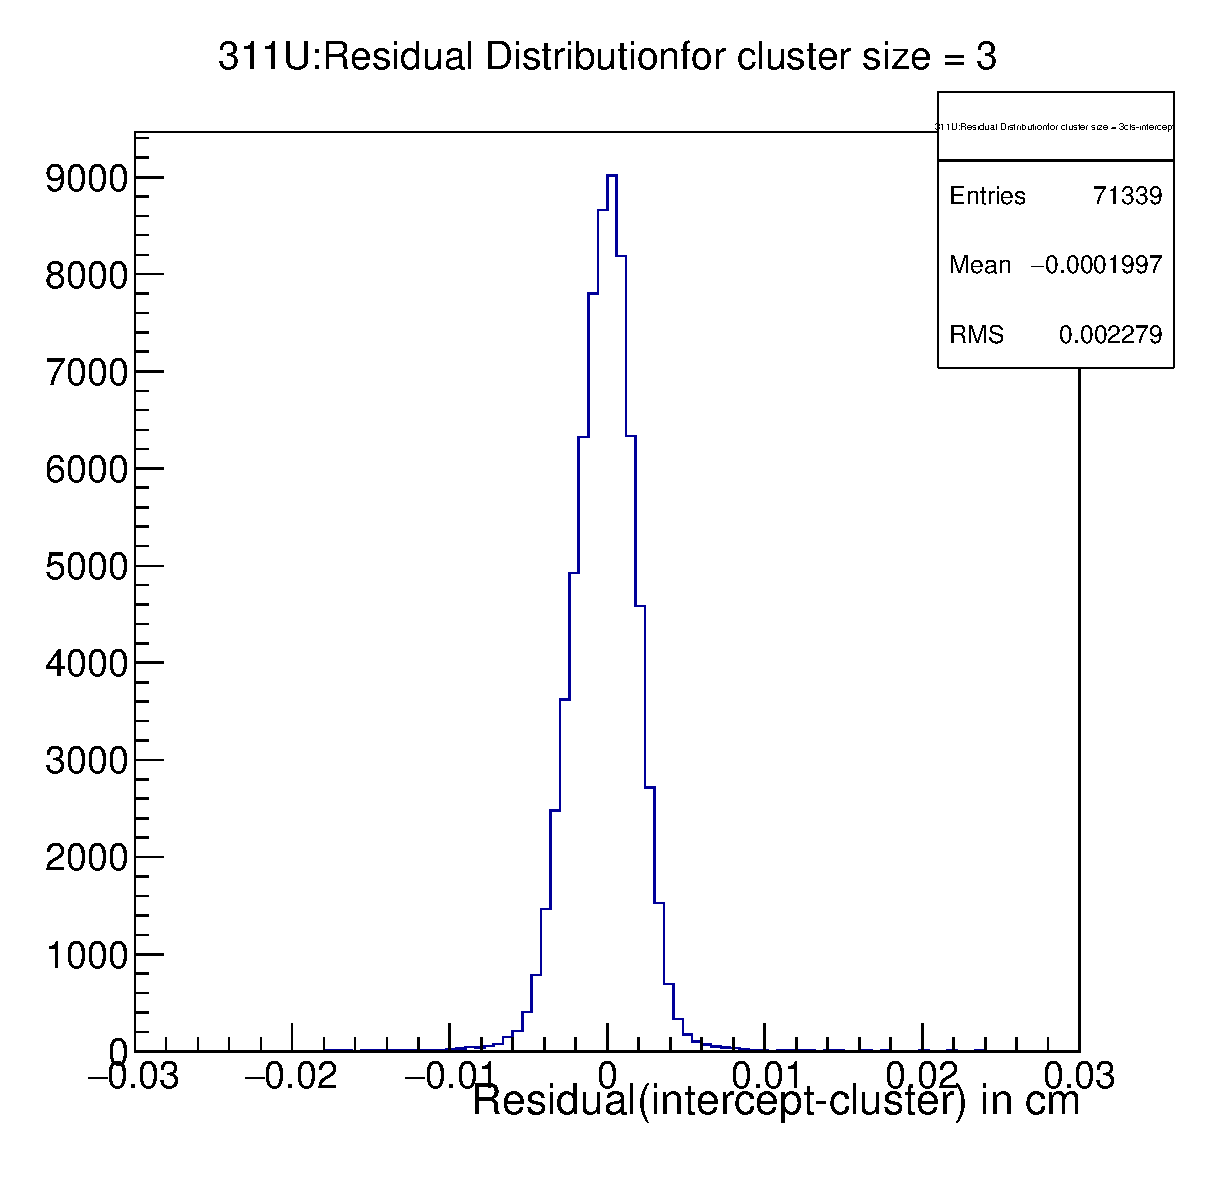
\includegraphics[width=.2\textwidth]{311U:clssize3.eps}	
					\caption{Residual distribution:Cluster size=3}	
					\label{fig2}	
				\end{figure}
					\begin{figure}[H]
						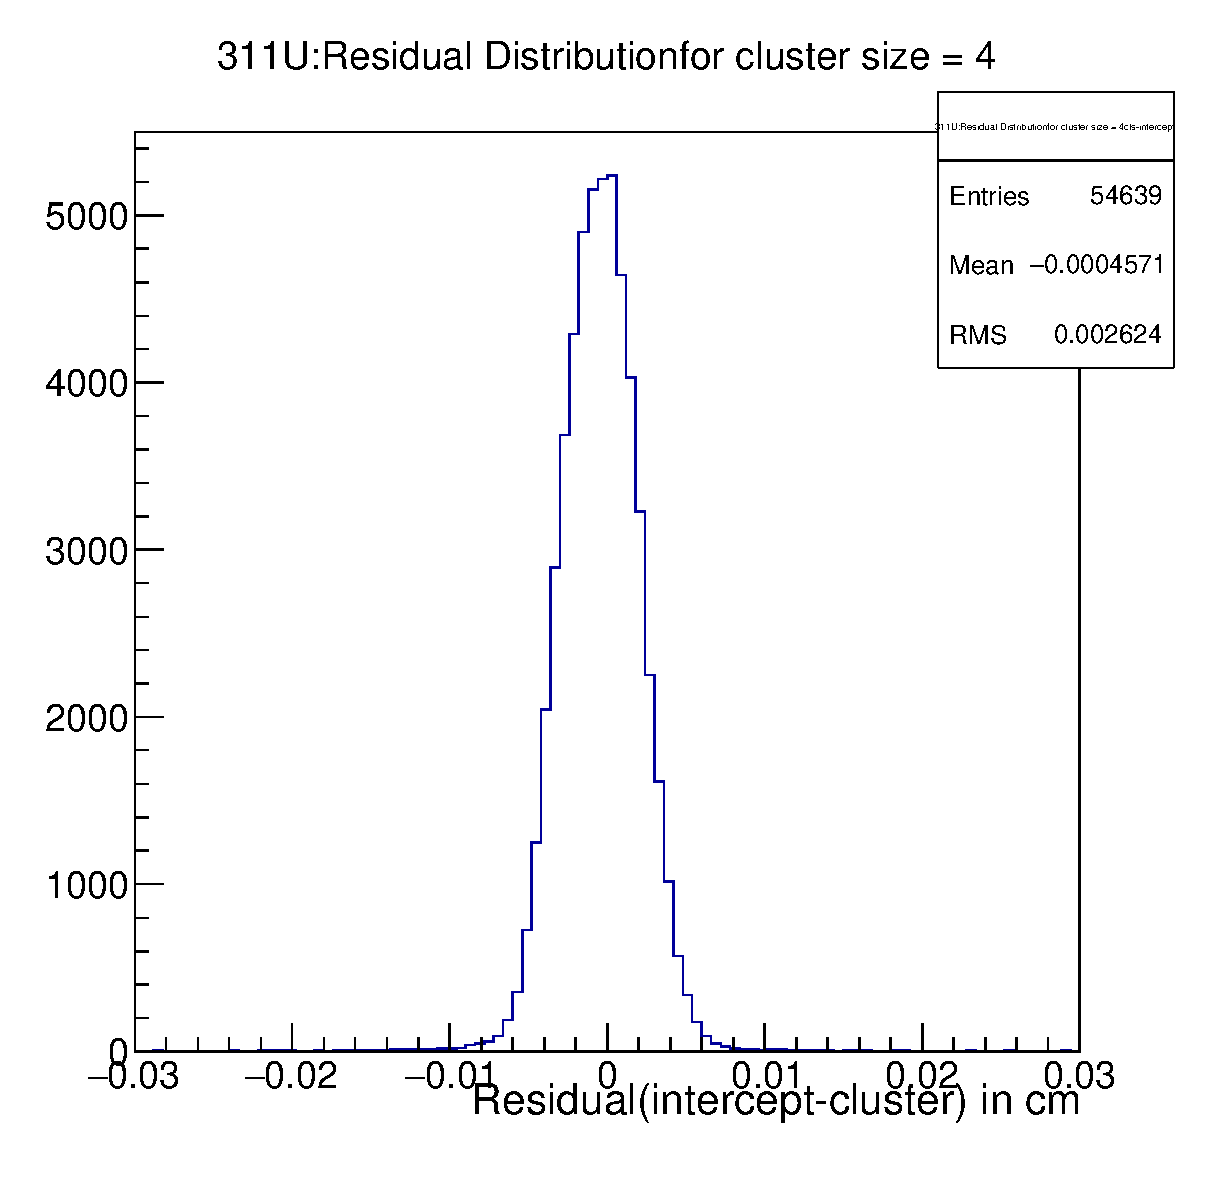
\includegraphics[width=.2\textwidth]{311U:clssize4.eps}	
						\caption{Residual distribution:Cluster size=4}	
						\label{fig2}	
					\end{figure}
		\end{multicols}
			\begin{figure}[H]
				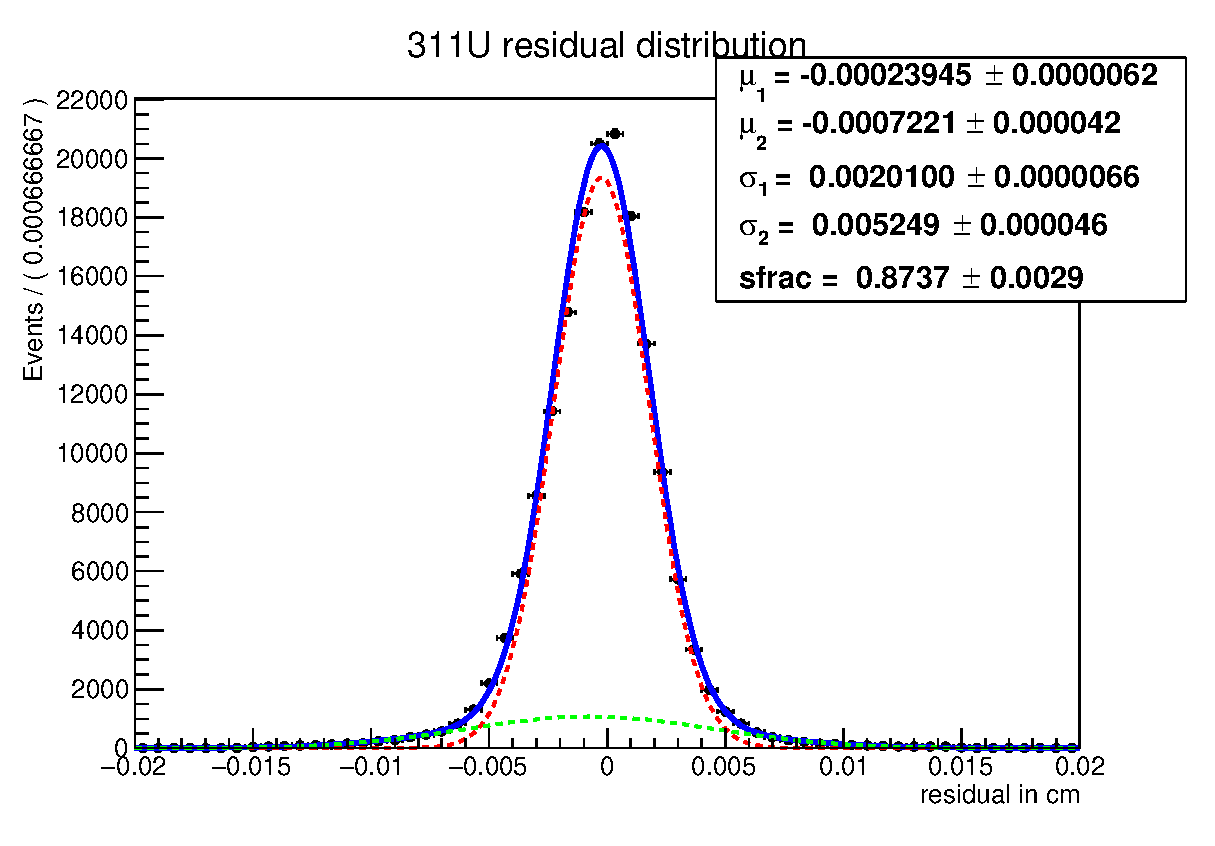
\includegraphics[width=.4\textwidth]{311U:fitted_residual.eps}	
				\caption{Residual distribution fitted with two Gaussian with different $\mu$ and $\sigma$ }	
				\label{fig2}	
			\end{figure}

		\pagebreak
			\subsubsection{Sensor:1 V\_side}
	\begin{multicols}{3}
		\begin{figure}[H]
			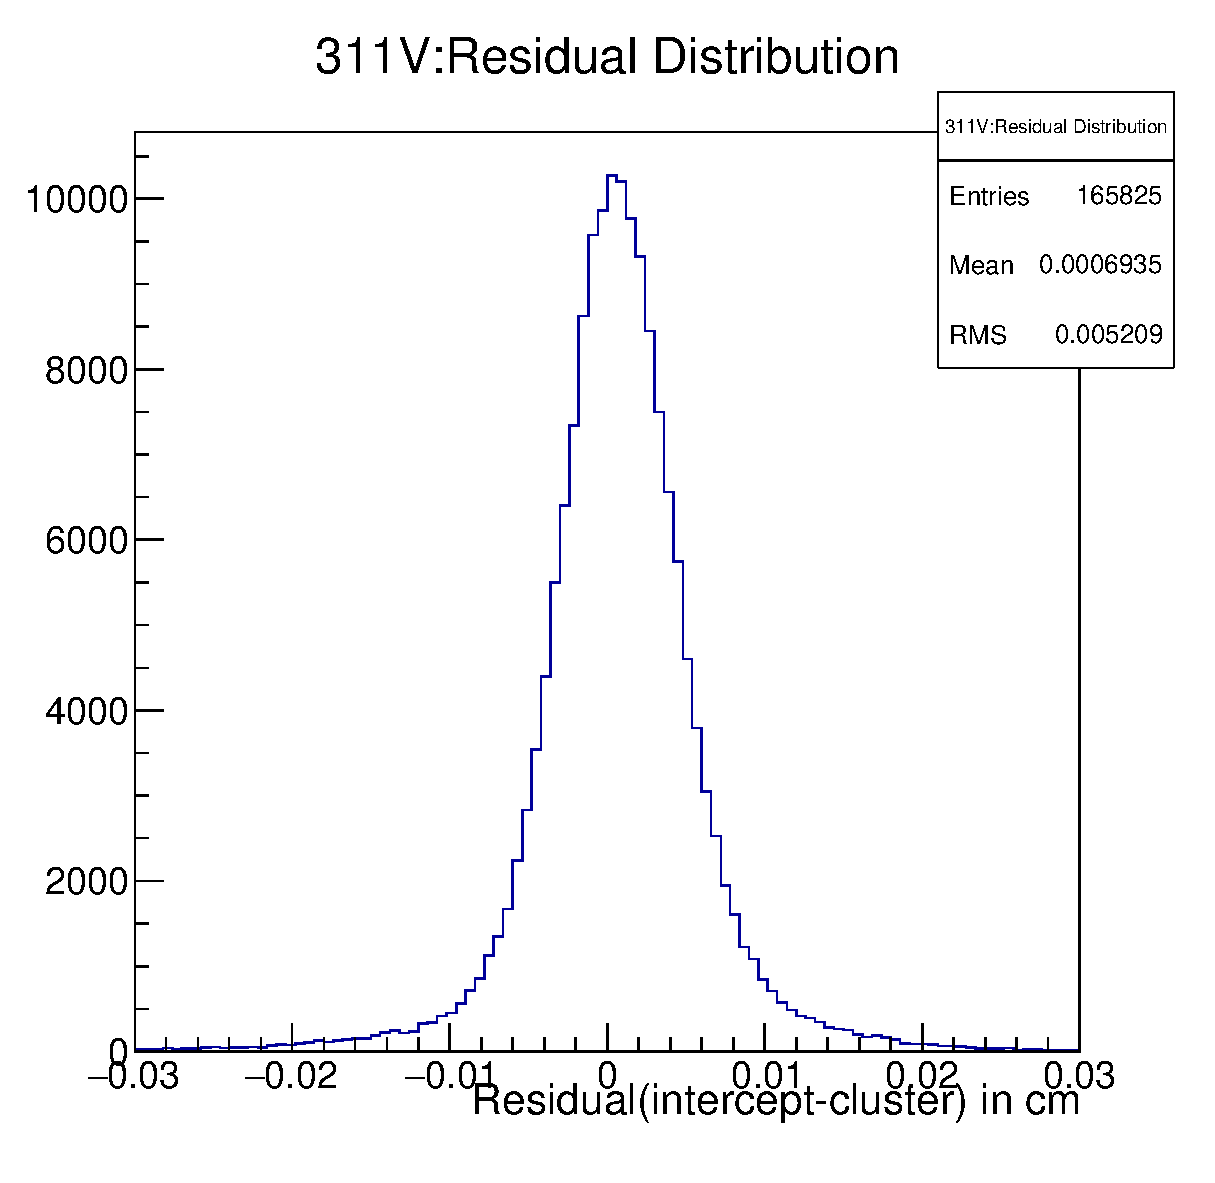
\includegraphics[width=.3\textwidth]{311V:residualplot.eps}	
			\caption{Residual distribution}	
			\label{fig1}	
		\end{figure}
		\begin{figure}[H]
			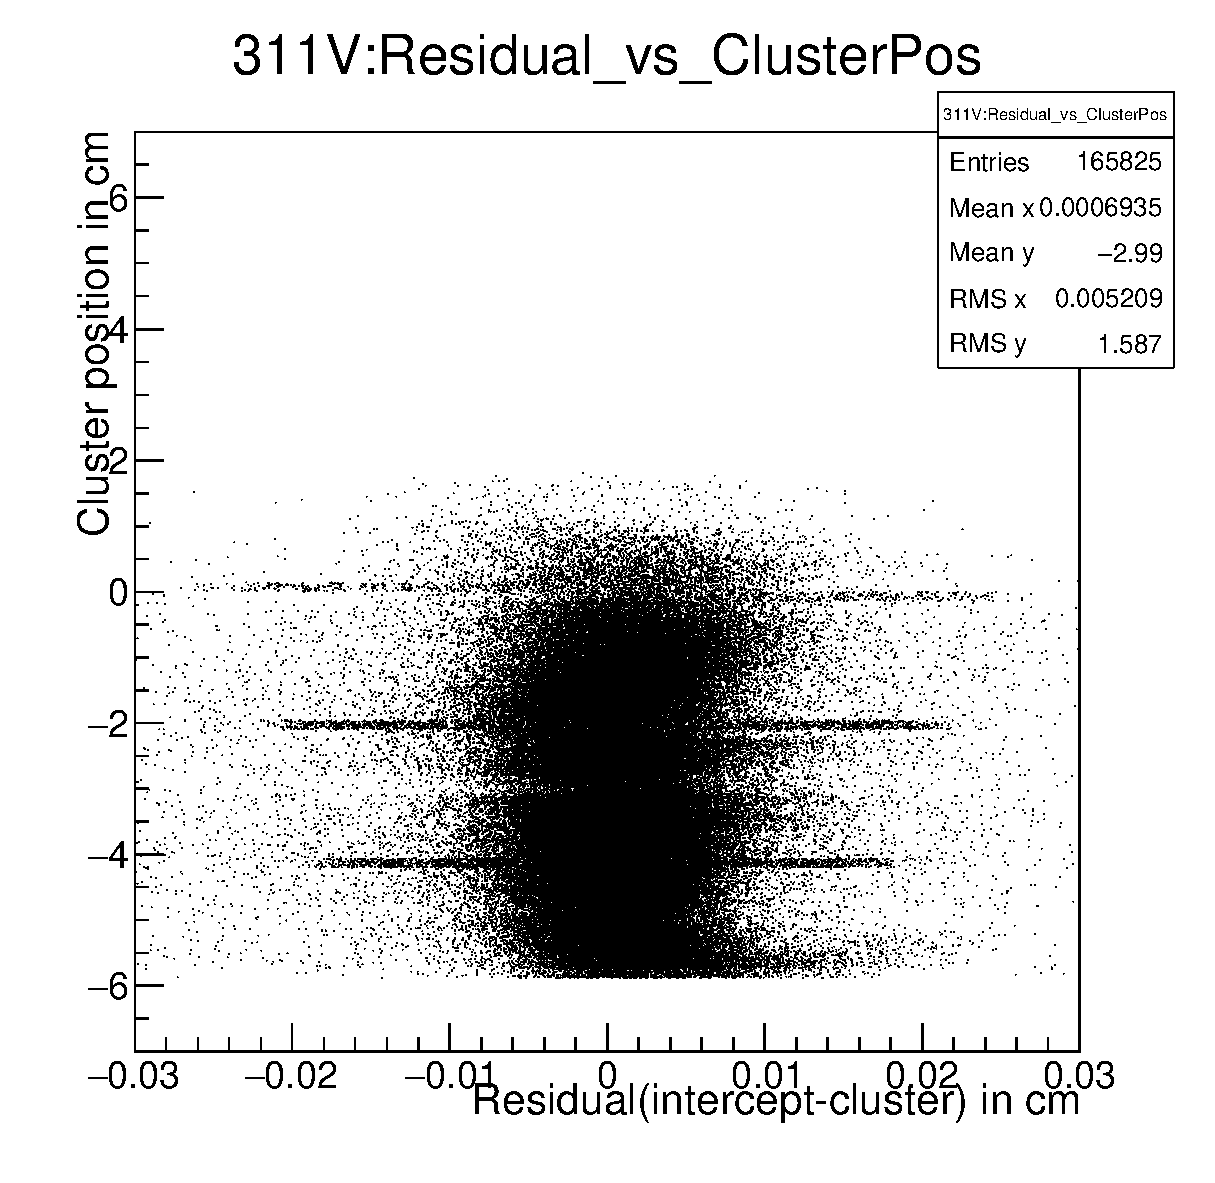
\includegraphics[width=.3\textwidth]{311V:residual_vs_clusterpos.eps}	
			\caption{Cluster position vs Residual}	
			\label{fig2}	
		\end{figure}
		\begin{figure}[H]
			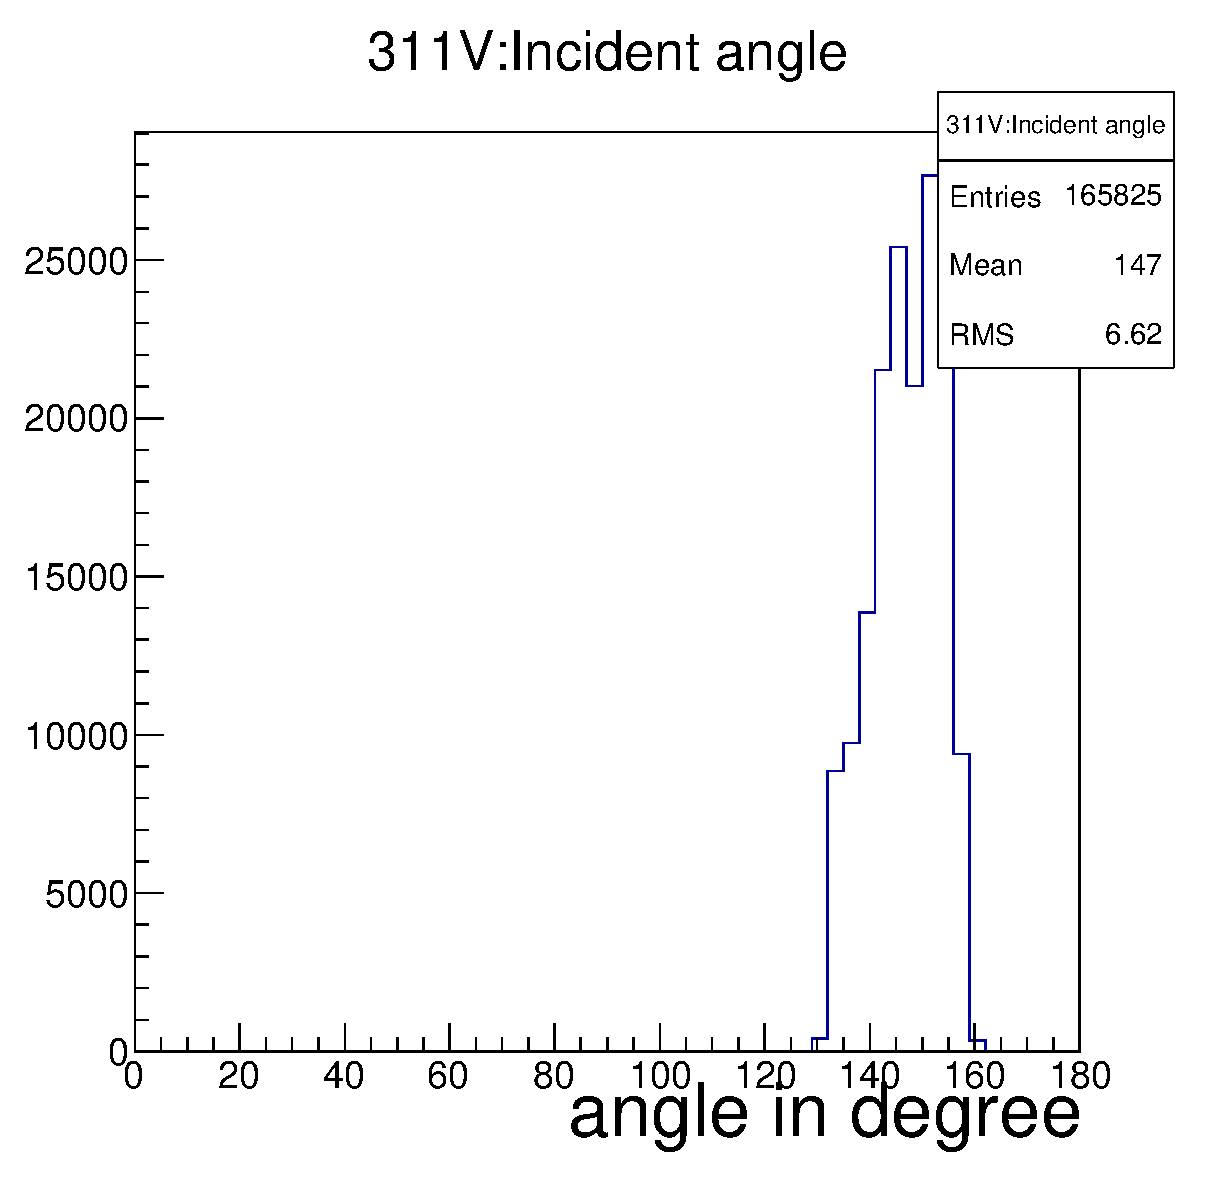
\includegraphics[width=.3\textwidth]{311V:incident_angle.eps}	
			\caption{Incident angle of the tracks}	
			\label{fig2}	
		\end{figure}
	\end{multicols}
	
	\begin{multicols}{4}
	
		\begin{figure}[H]
			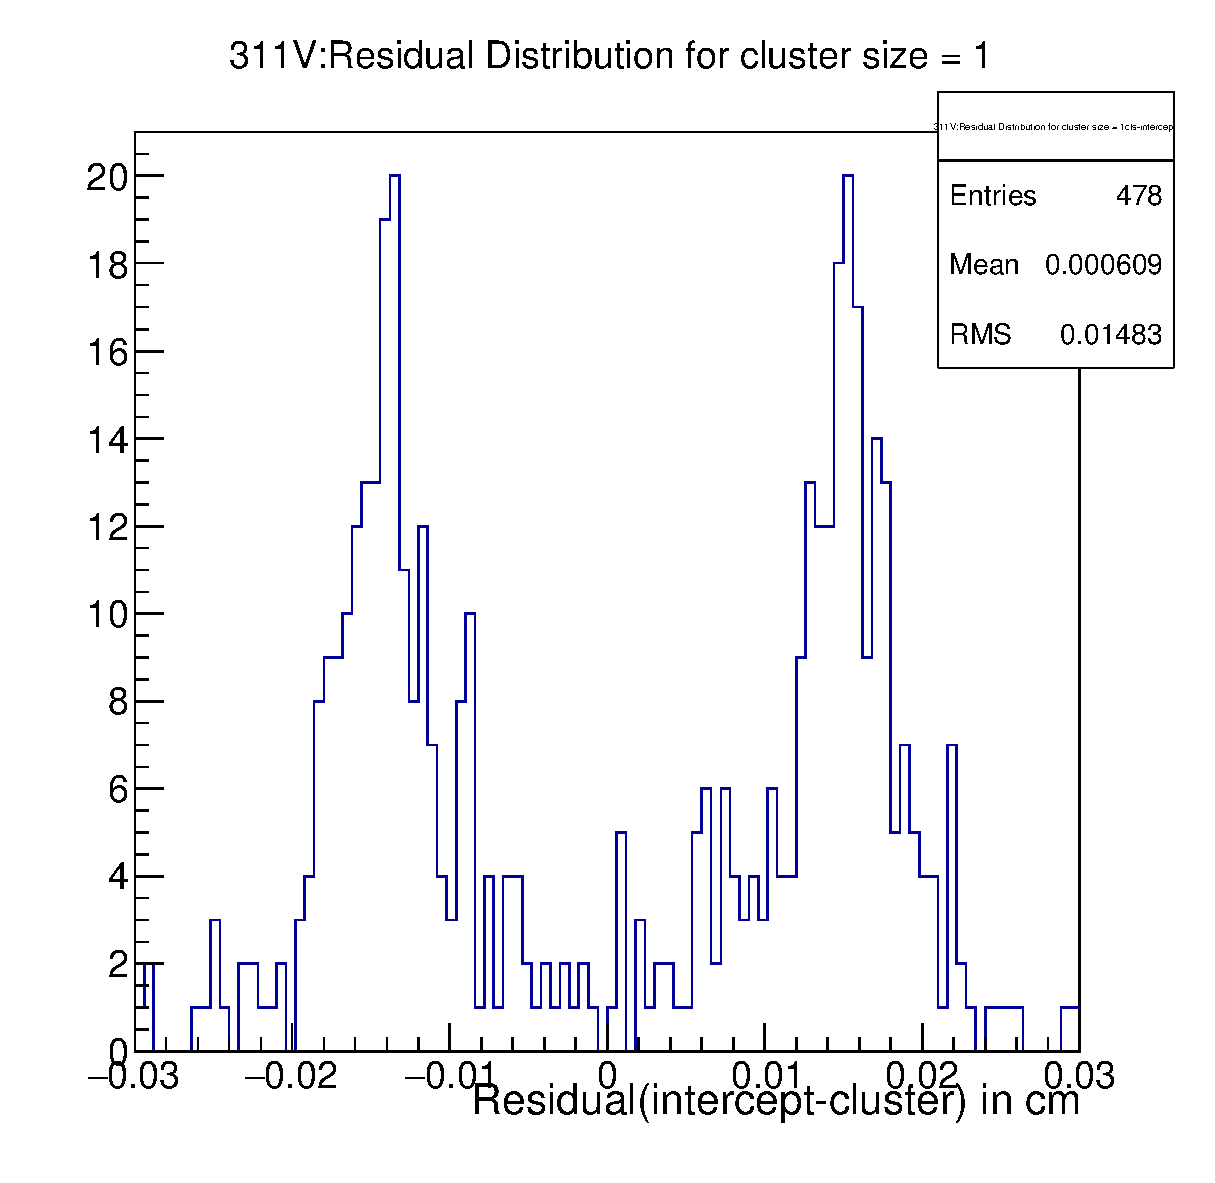
\includegraphics[width=.2\textwidth]{311V:clssize1.eps}	
			\caption{Residual distribution:Cluster size=1}	
			\label{fig1}	
		\end{figure}
		\begin{figure}[H]
			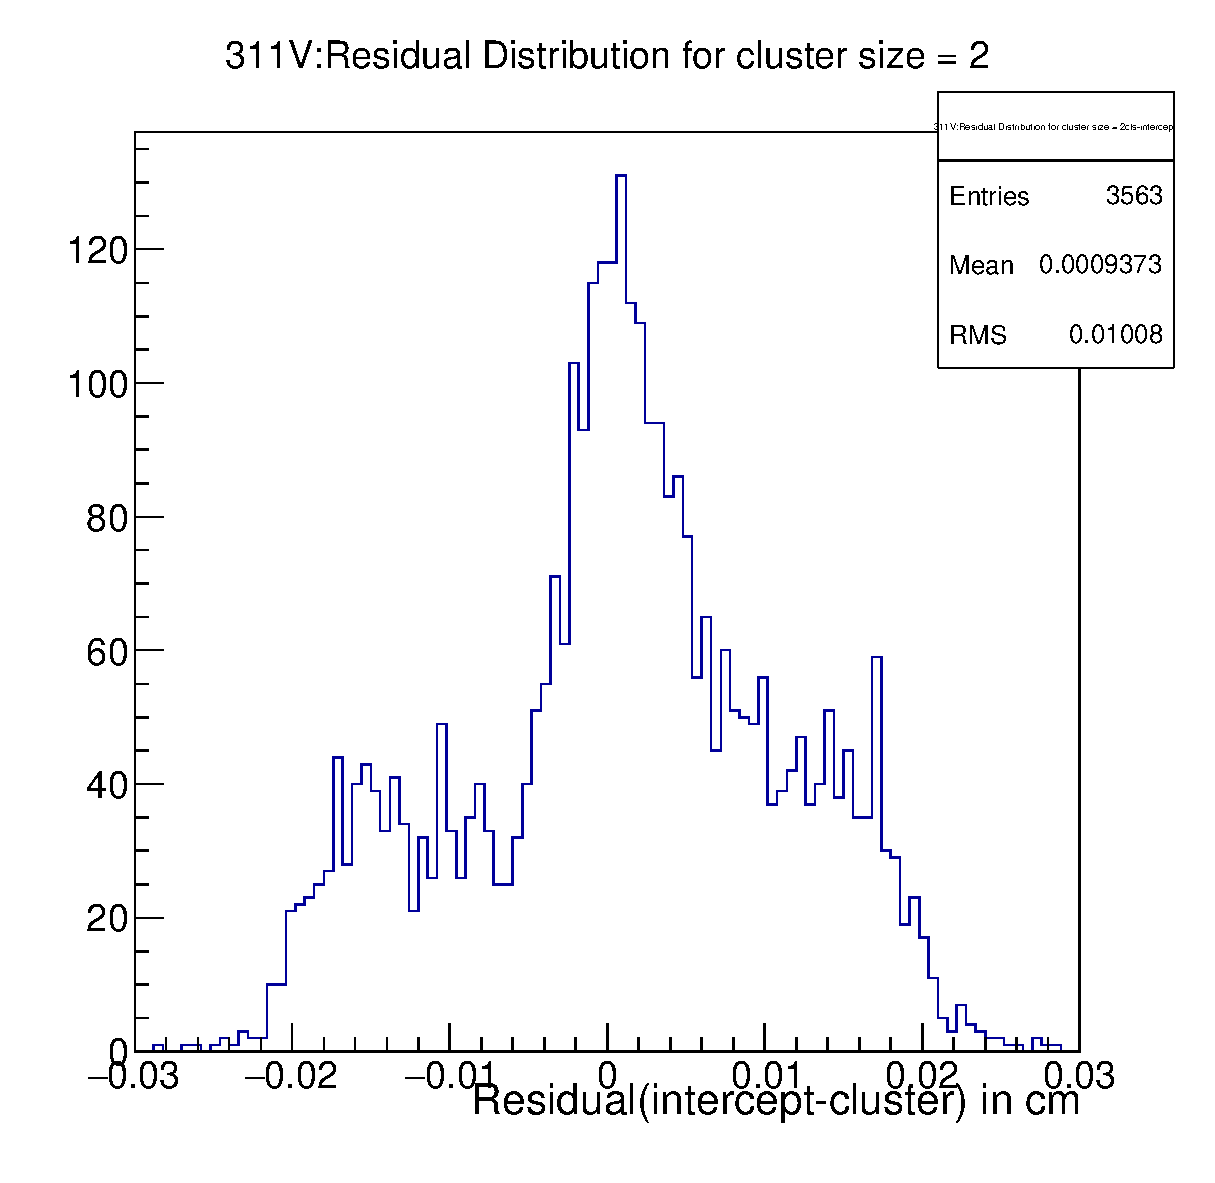
\includegraphics[width=.2\textwidth]{311V:clssize2.eps}	
			\caption{Residual distribution:Cluster size=2}	
			\label{fig2}	
		\end{figure}
		\begin{figure}[H]
			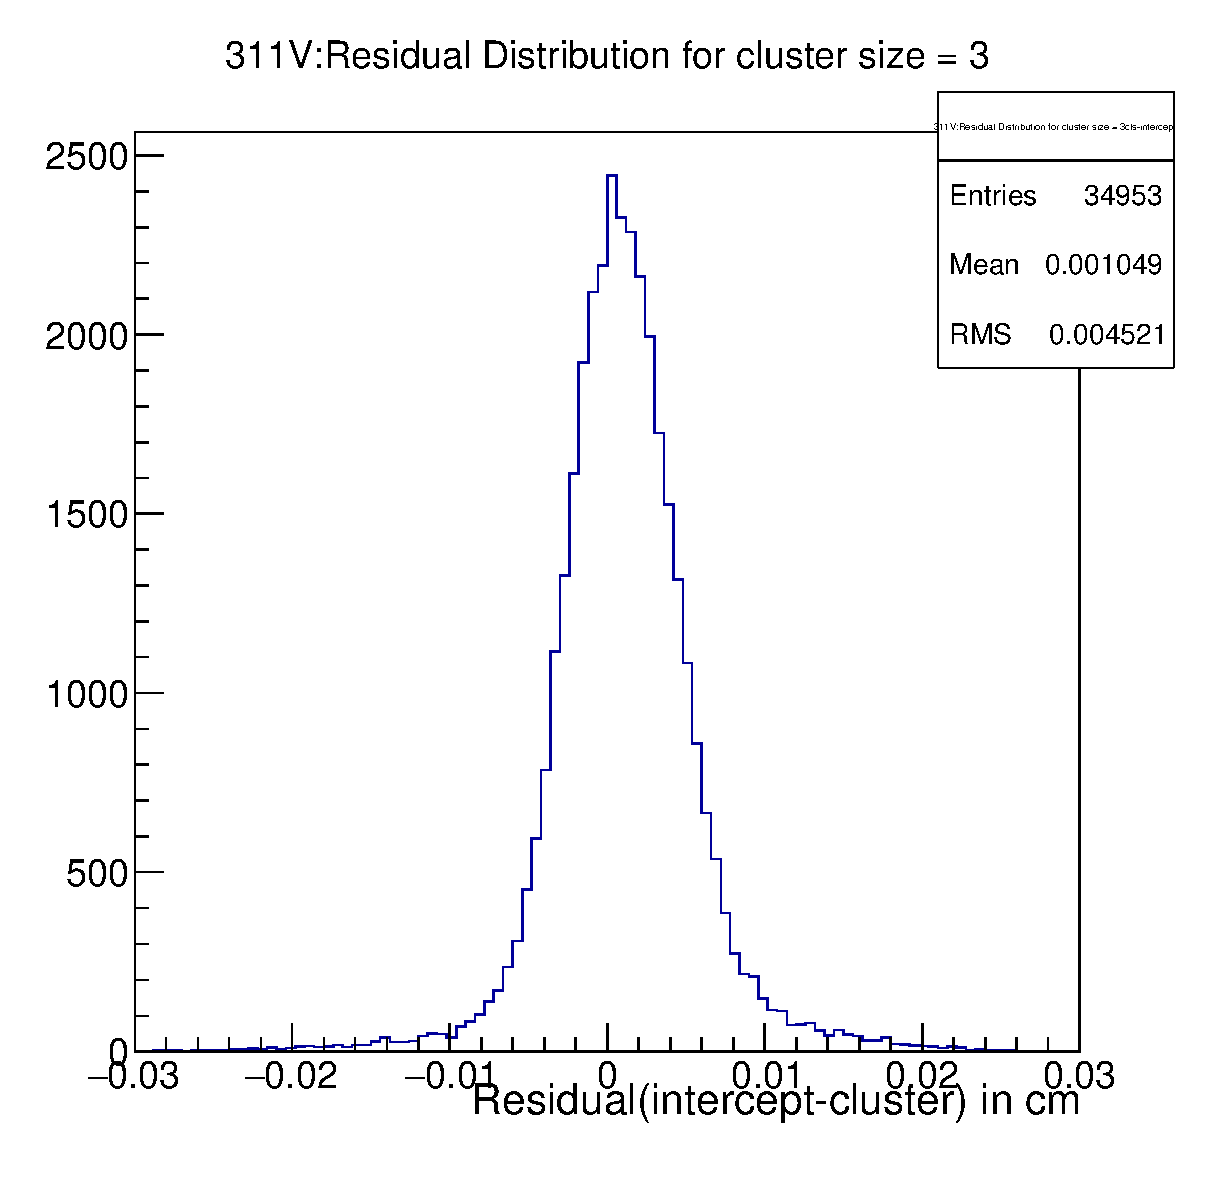
\includegraphics[width=.2\textwidth]{311V:clssize3.eps}	
			\caption{Residual distribution:Cluster size=3}	
			\label{fig2}	
		\end{figure}
		\begin{figure}[H]
			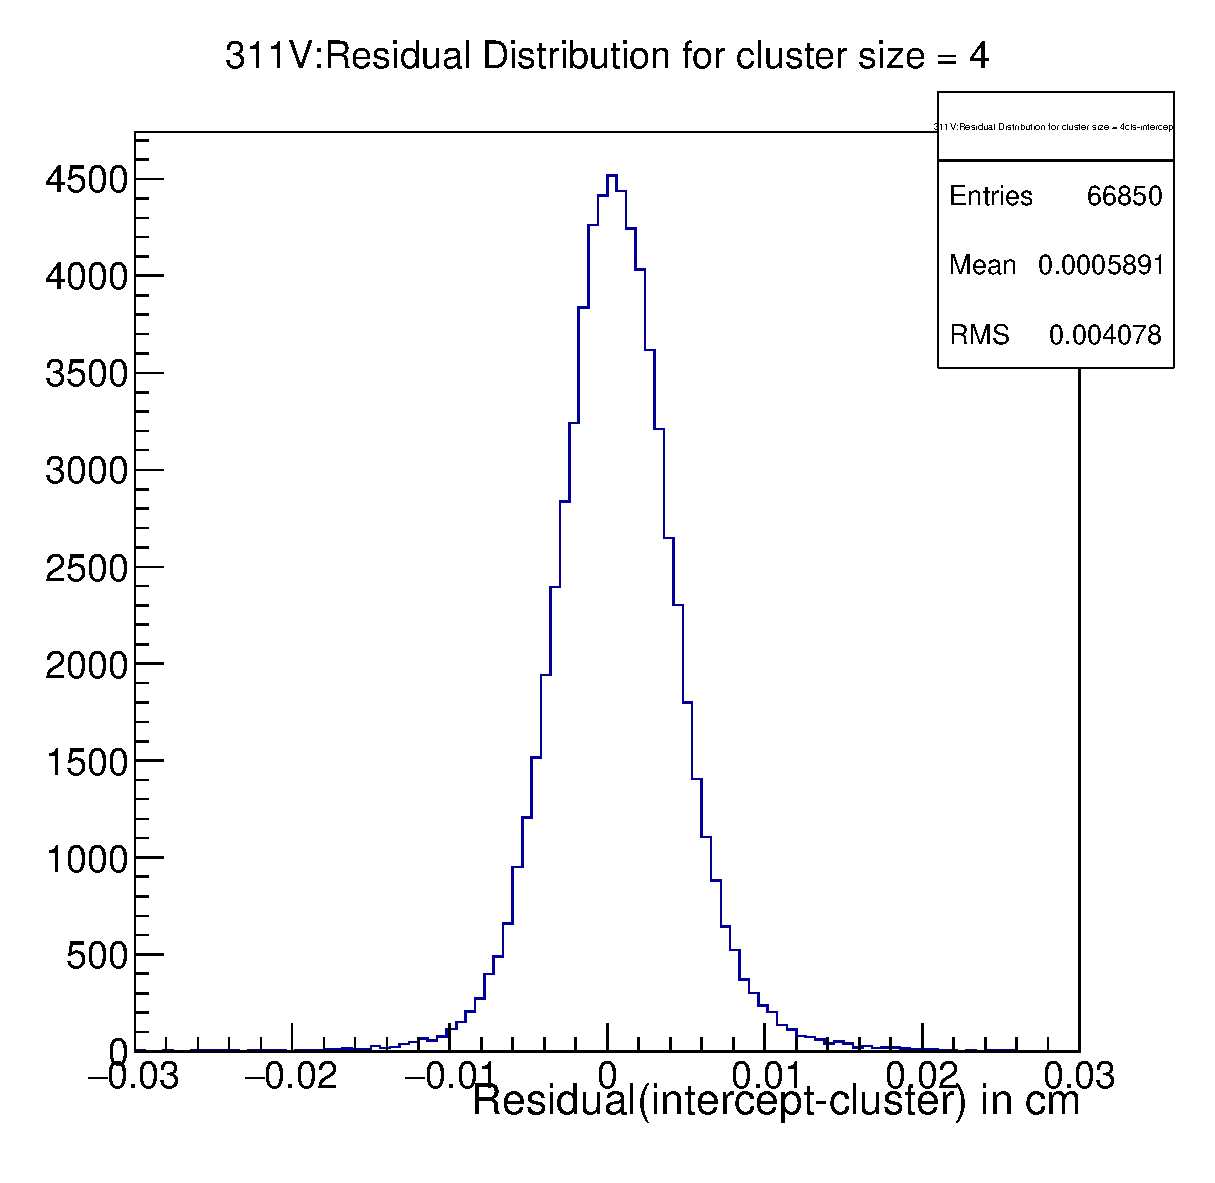
\includegraphics[width=.2\textwidth]{311V:clssize4.eps}	
			\caption{Residual distribution:Cluster size=4}	
			\label{fig2}	
		\end{figure}
	\end{multicols}
		\begin{figure}[H]
			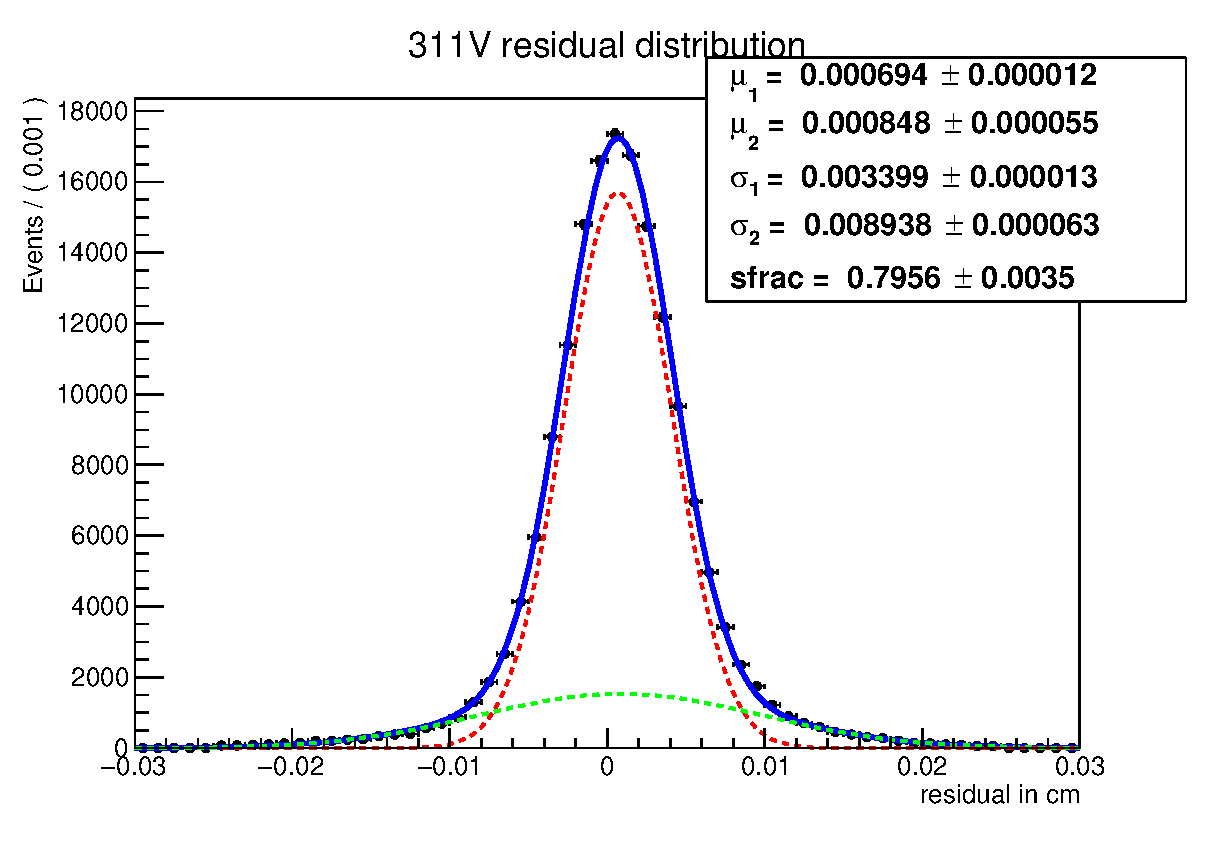
\includegraphics[width=.4\textwidth]{311V:fitted_residual.eps}	
			\caption{Residual distribution fitted with two Gaussian with different $\mu$ and $\sigma$ }	
			\label{fig2}	
		\end{figure}
	\pagebreak

	\subsubsection{Sensor:2 U\_side}
	\begin{multicols}{3}
		
		\begin{figure}[H]
			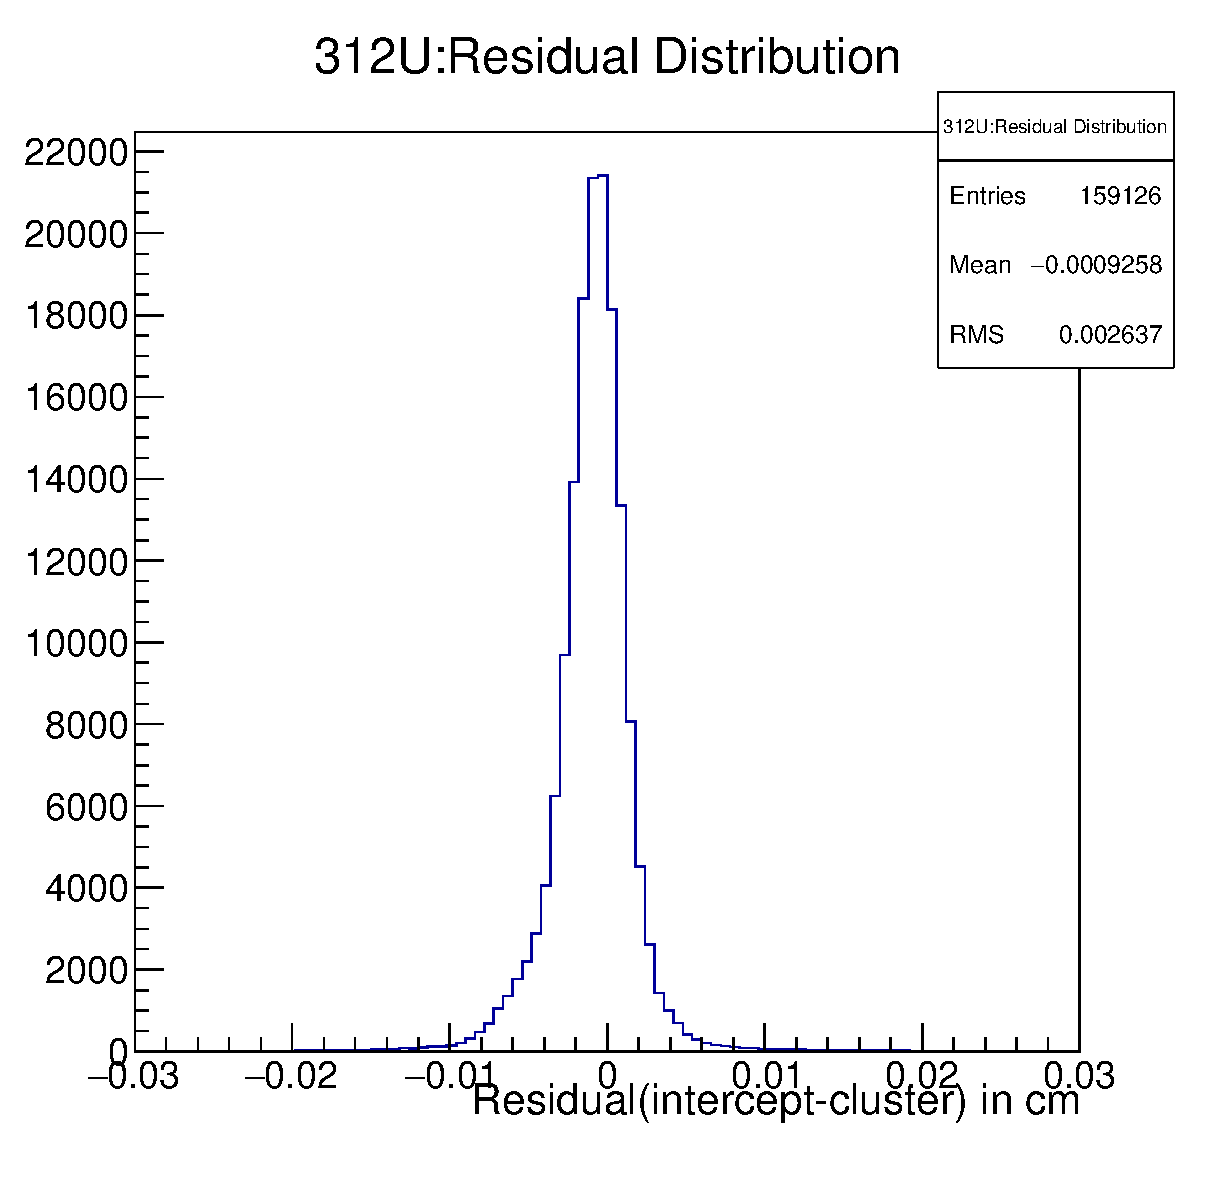
\includegraphics[width=.3\textwidth]{312U:residualplot.eps}	
			\caption{Residual distribution}	
			\label{fig1}	
		\end{figure}
		\begin{figure}[H]
			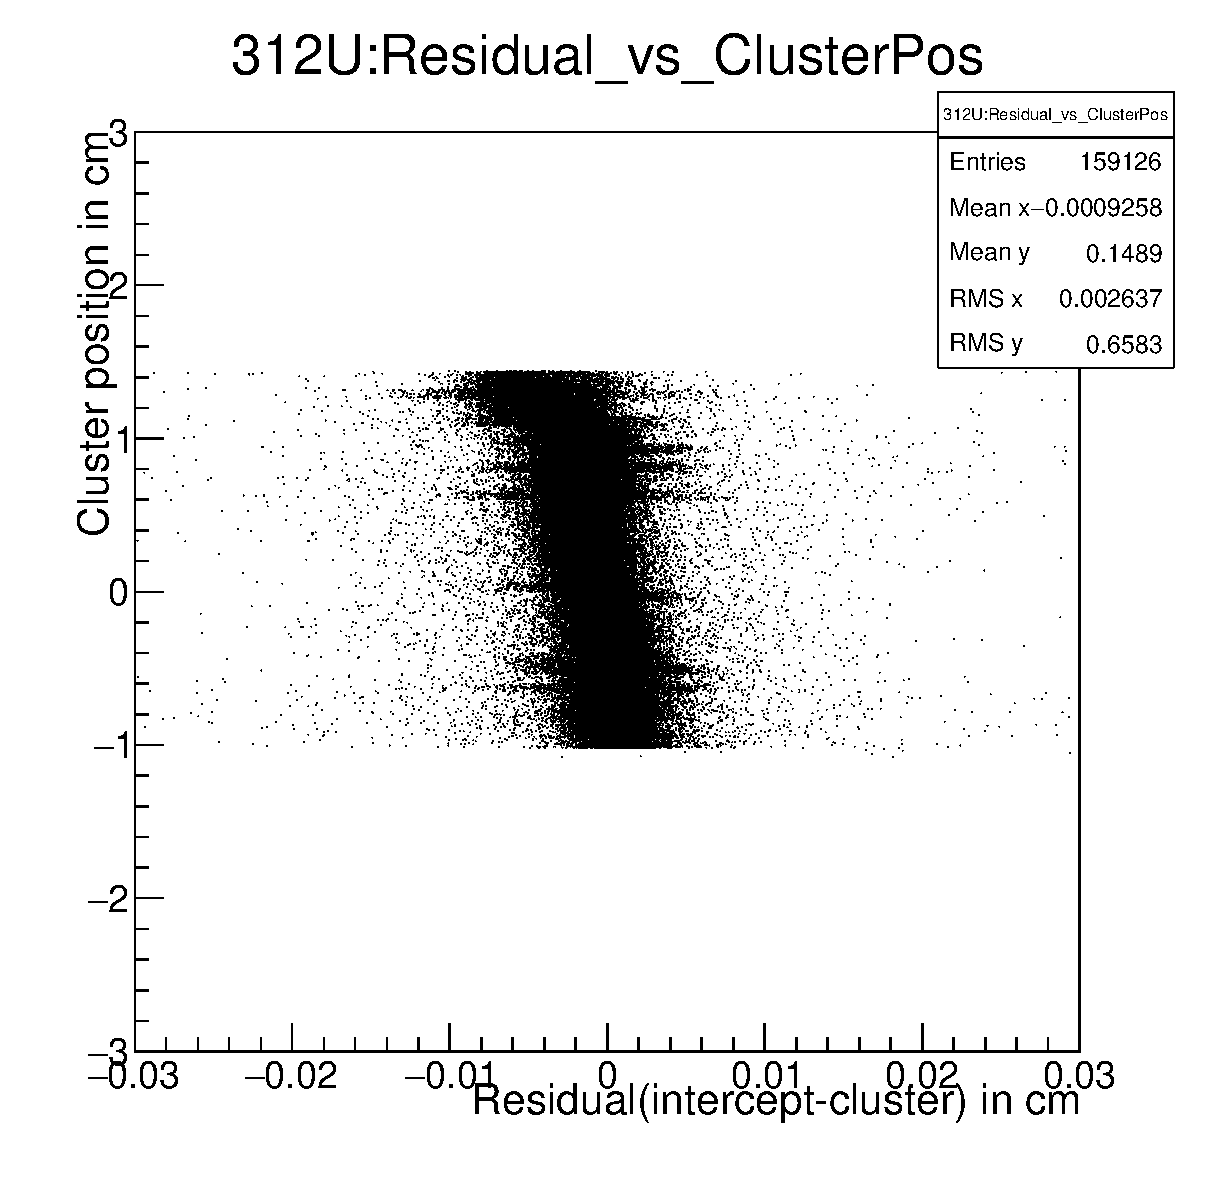
\includegraphics[width=.3\textwidth]{312U:residual_vs_clusterpos.eps}	
			\caption{Cluster position vs Residual}	
			\label{fig2}	
		\end{figure}
		\begin{figure}[H]
			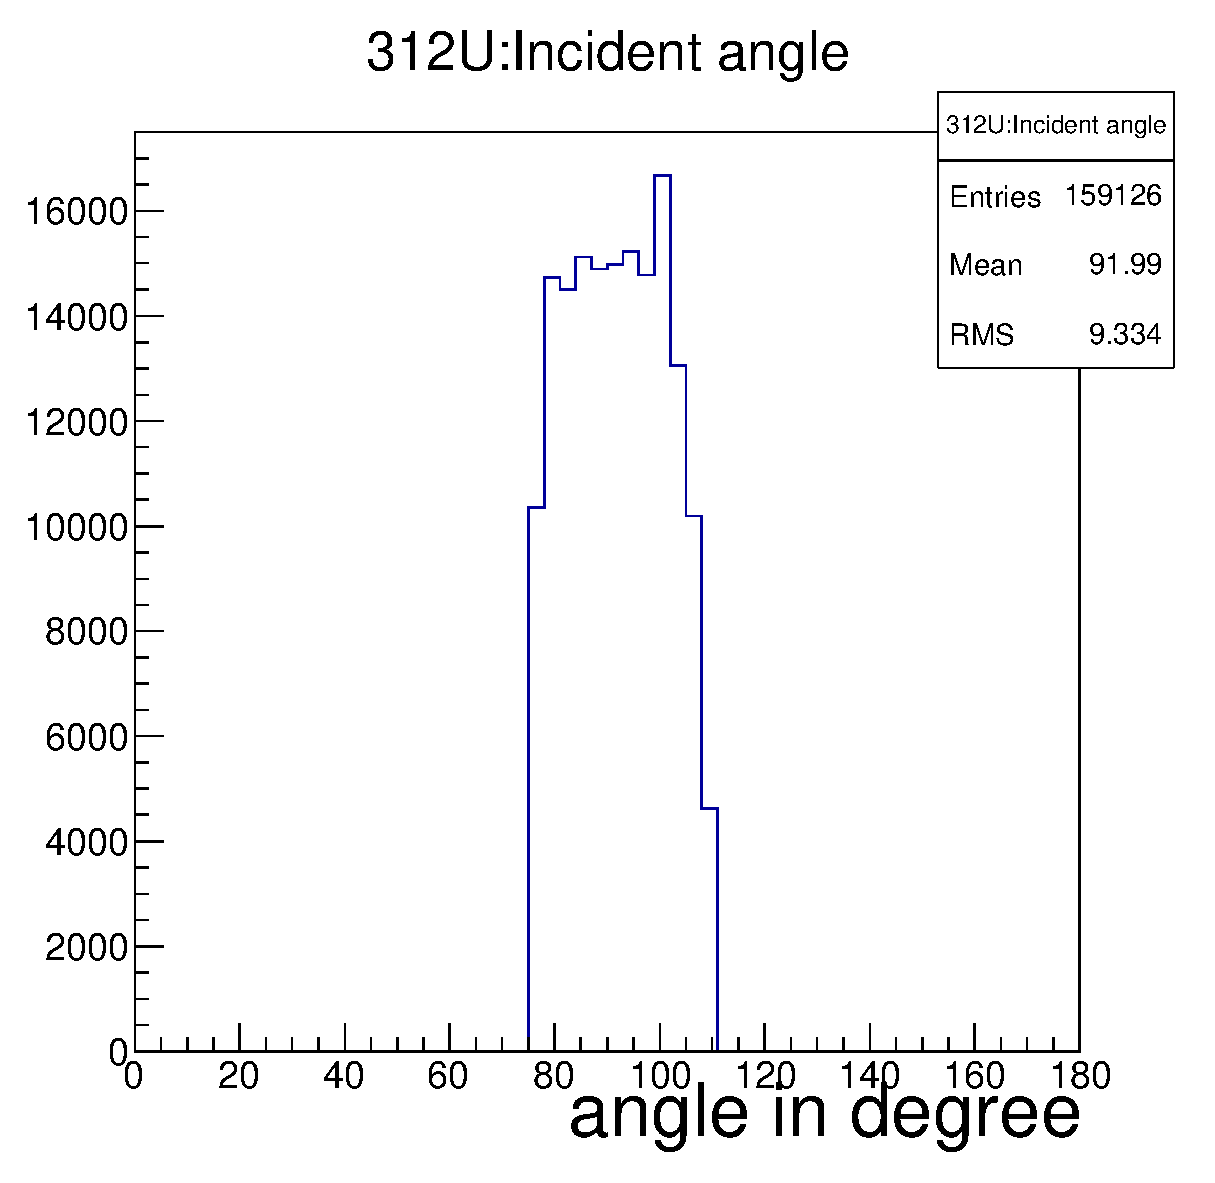
\includegraphics[width=.3\textwidth]{312U:incident_angle.eps}	
			\caption{Incident angle of the tracks}	
			\label{fig2}	
		\end{figure}
	\end{multicols}
	
	\begin{multicols}{4}
		
		\begin{figure}[H]
			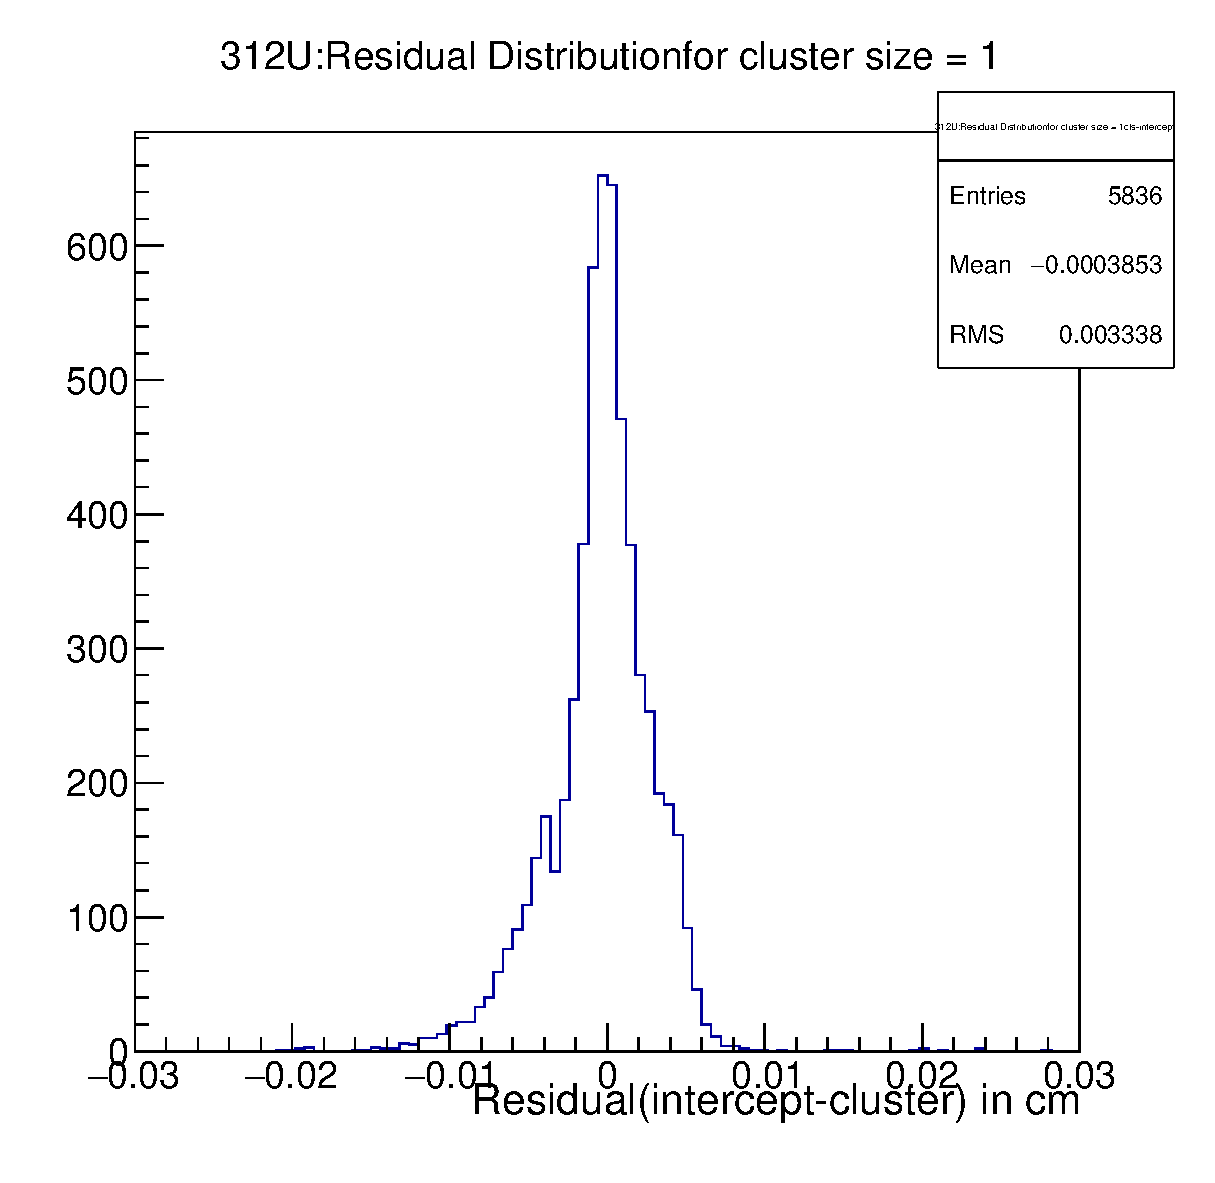
\includegraphics[width=.2\textwidth]{312U:clssize1.eps}	
			\caption{Residual distribution:Cluster size=1}	
			\label{fig1}	
		\end{figure}
		\begin{figure}[H]
			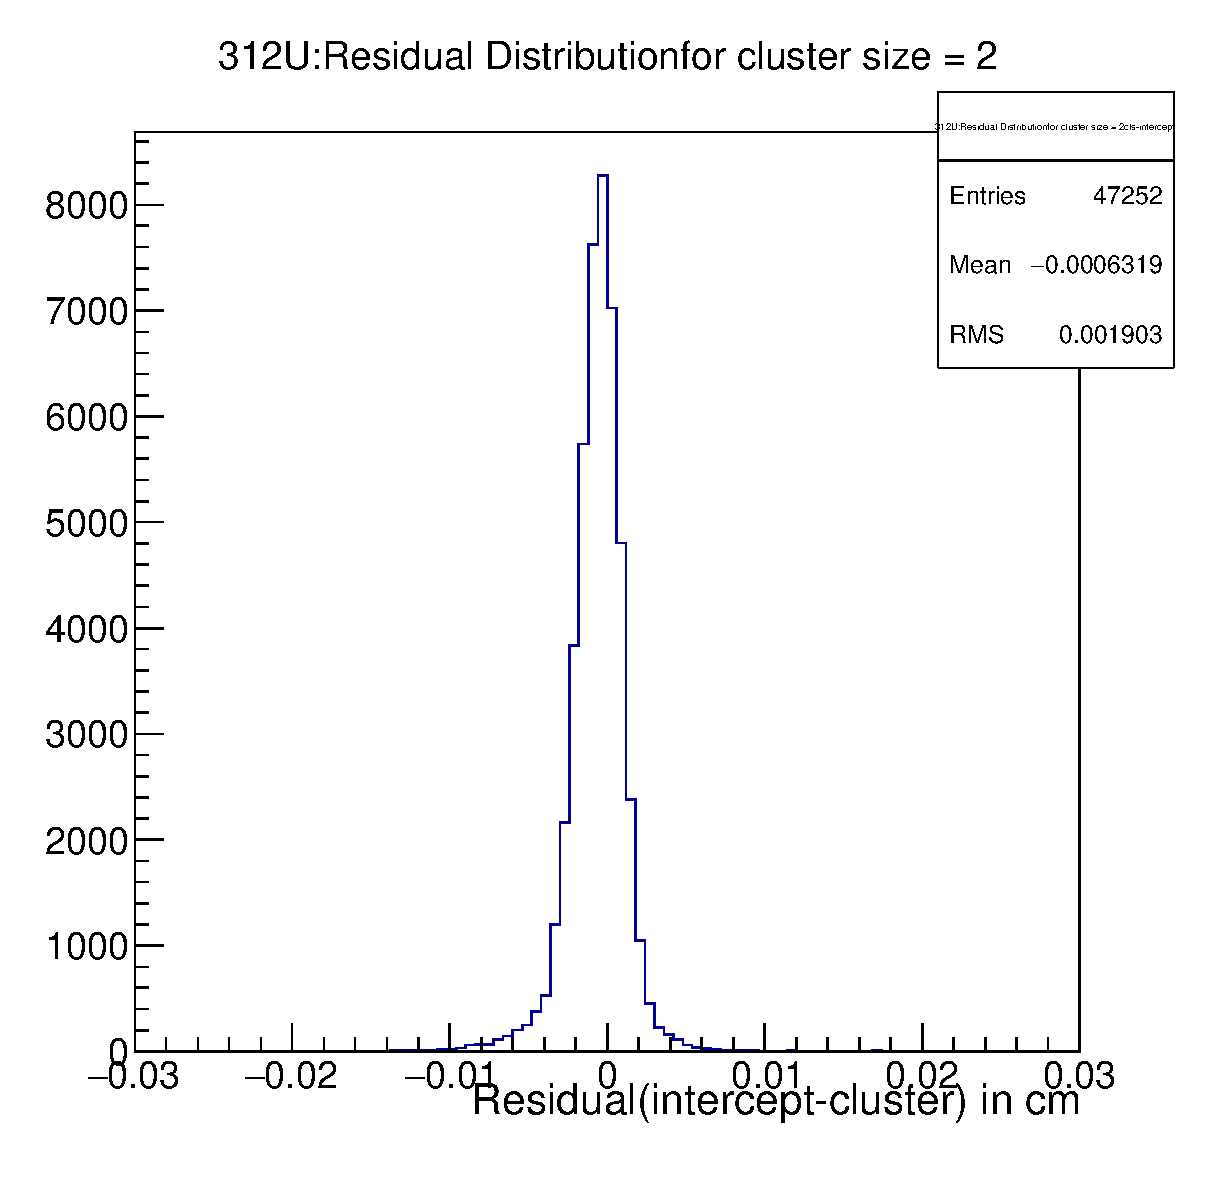
\includegraphics[width=.2\textwidth]{312U:clssize2.eps}	
			\caption{Residual distribution:Cluster size=2}	
			\label{fig2}	
		\end{figure}
		\begin{figure}[H]
			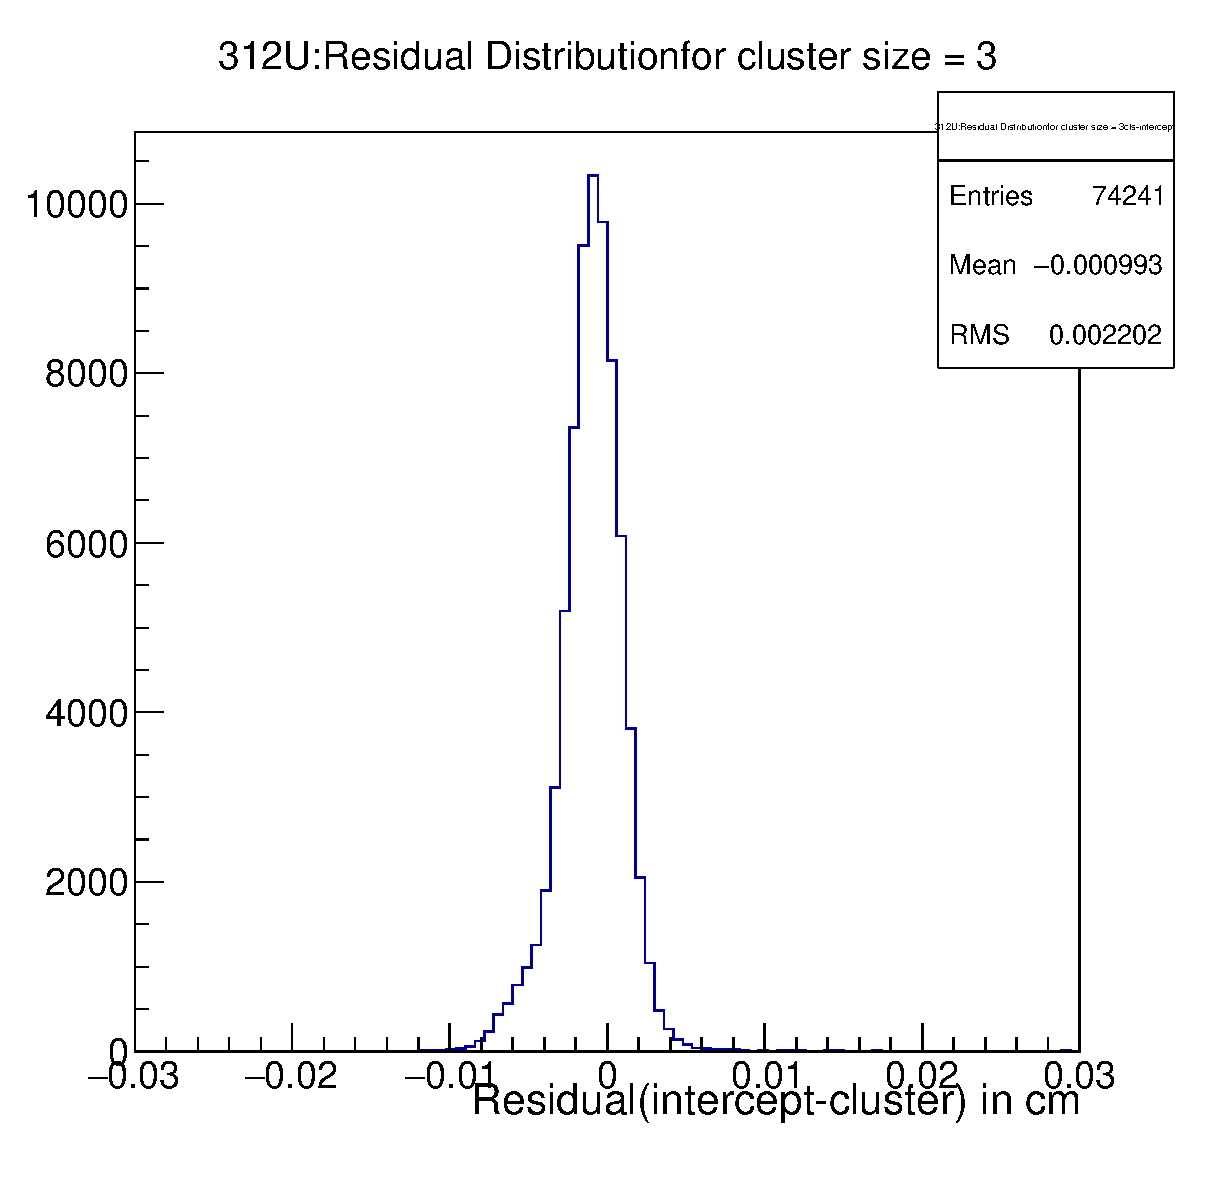
\includegraphics[width=.2\textwidth]{312U:clssize3.eps}	
			\caption{Residual distribution:Cluster size=3}	
			\label{fig2}	
		\end{figure}
		\begin{figure}[H]
			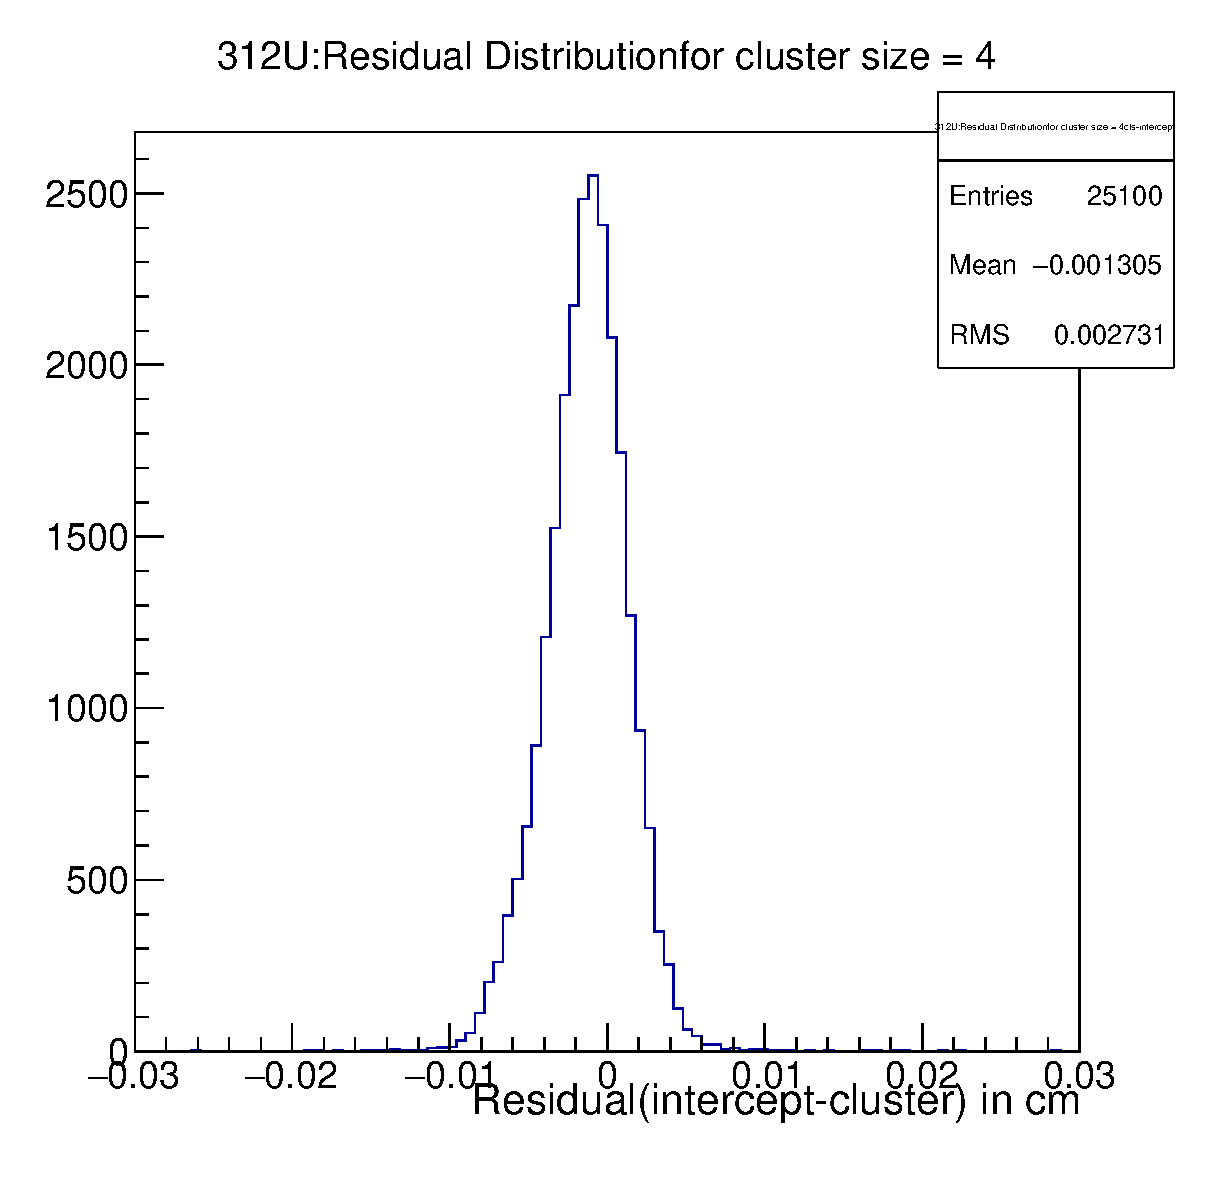
\includegraphics[width=.2\textwidth]{312U:clssize4.eps}	
			\caption{Residual distribution:Cluster size=4}	
			\label{fig2}	
		\end{figure}
	\end{multicols}
		\begin{figure}[H]
			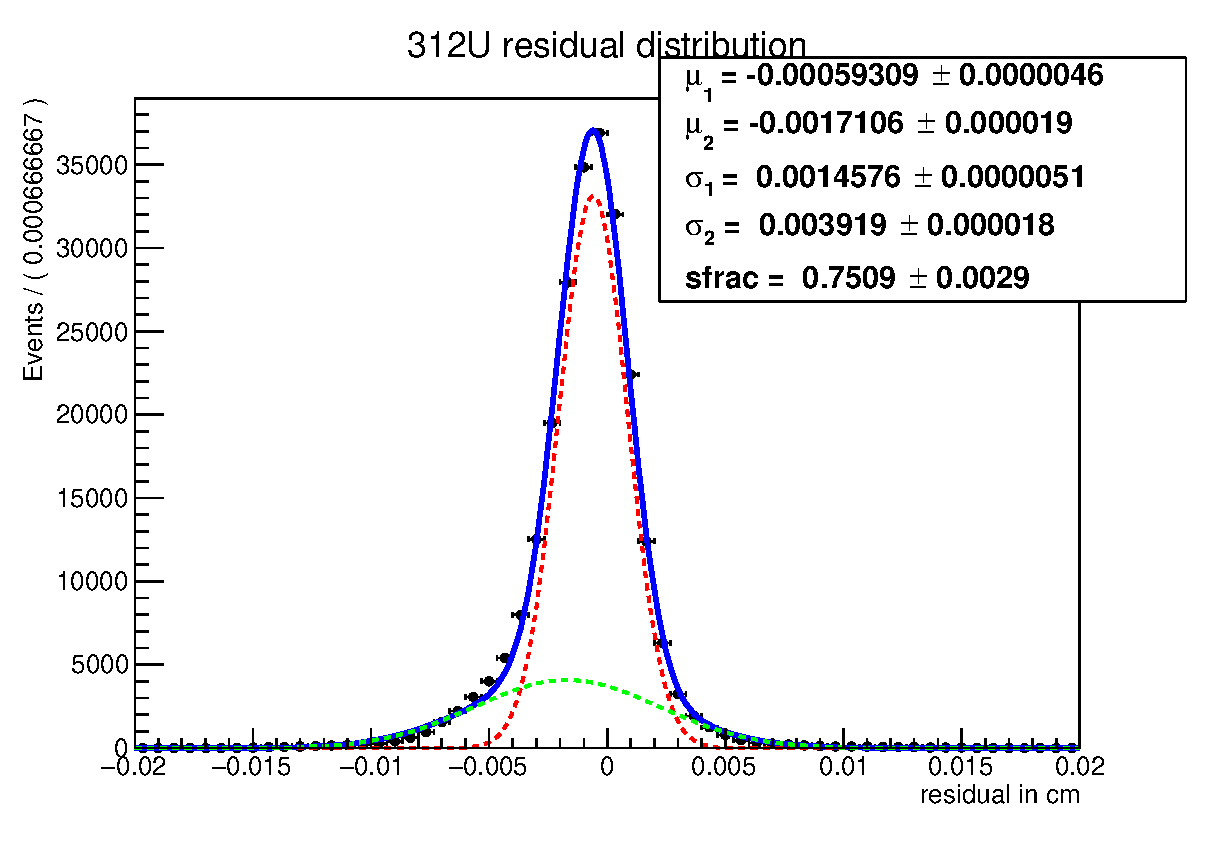
\includegraphics[width=.4\textwidth]{312U:fitted_residual.eps}	
			\caption{Residual distribution fitted with two Gaussian with different $\mu$ and $\sigma$ }	
			\label{fig2}	
		\end{figure}
	\pagebreak
	\subsubsection{Sensor:2 V\_side}
	\begin{multicols}{3}
		\begin{figure}[H]
			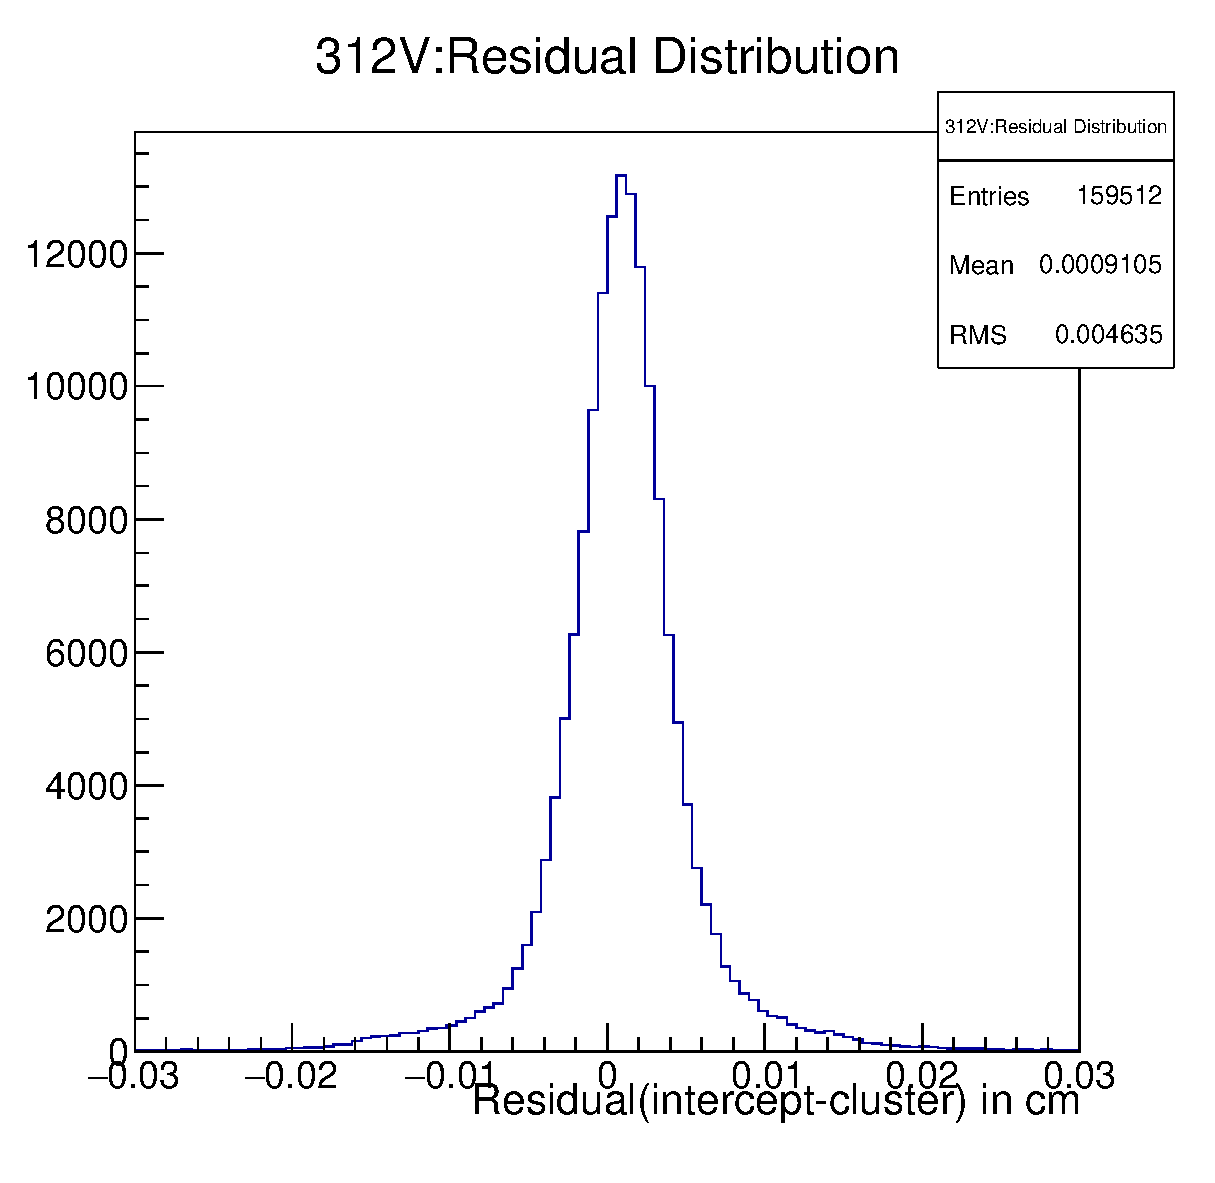
\includegraphics[width=.3\textwidth]{312V:residualplot.eps}	
			\caption{Residual distribution}	
			\label{fig1}	
		\end{figure}
		\begin{figure}[H]
			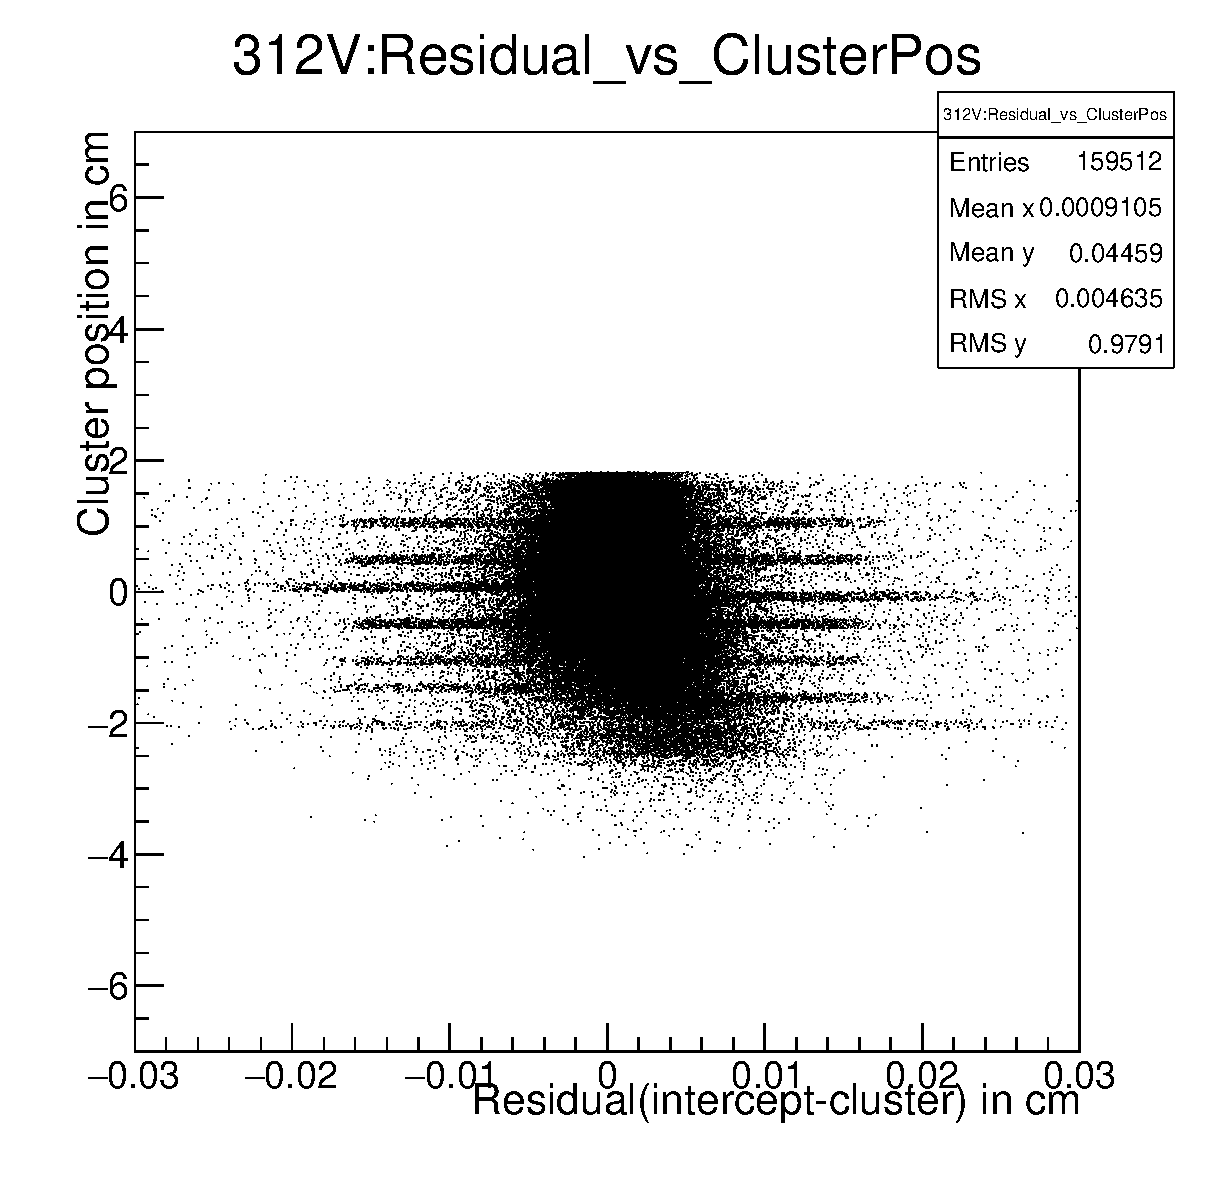
\includegraphics[width=.3\textwidth]{312V:residual_vs_clusterpos.eps}	
			\caption{Cluster position vs Residual}	
			\label{fig2}	
		\end{figure}
		\begin{figure}[H]
			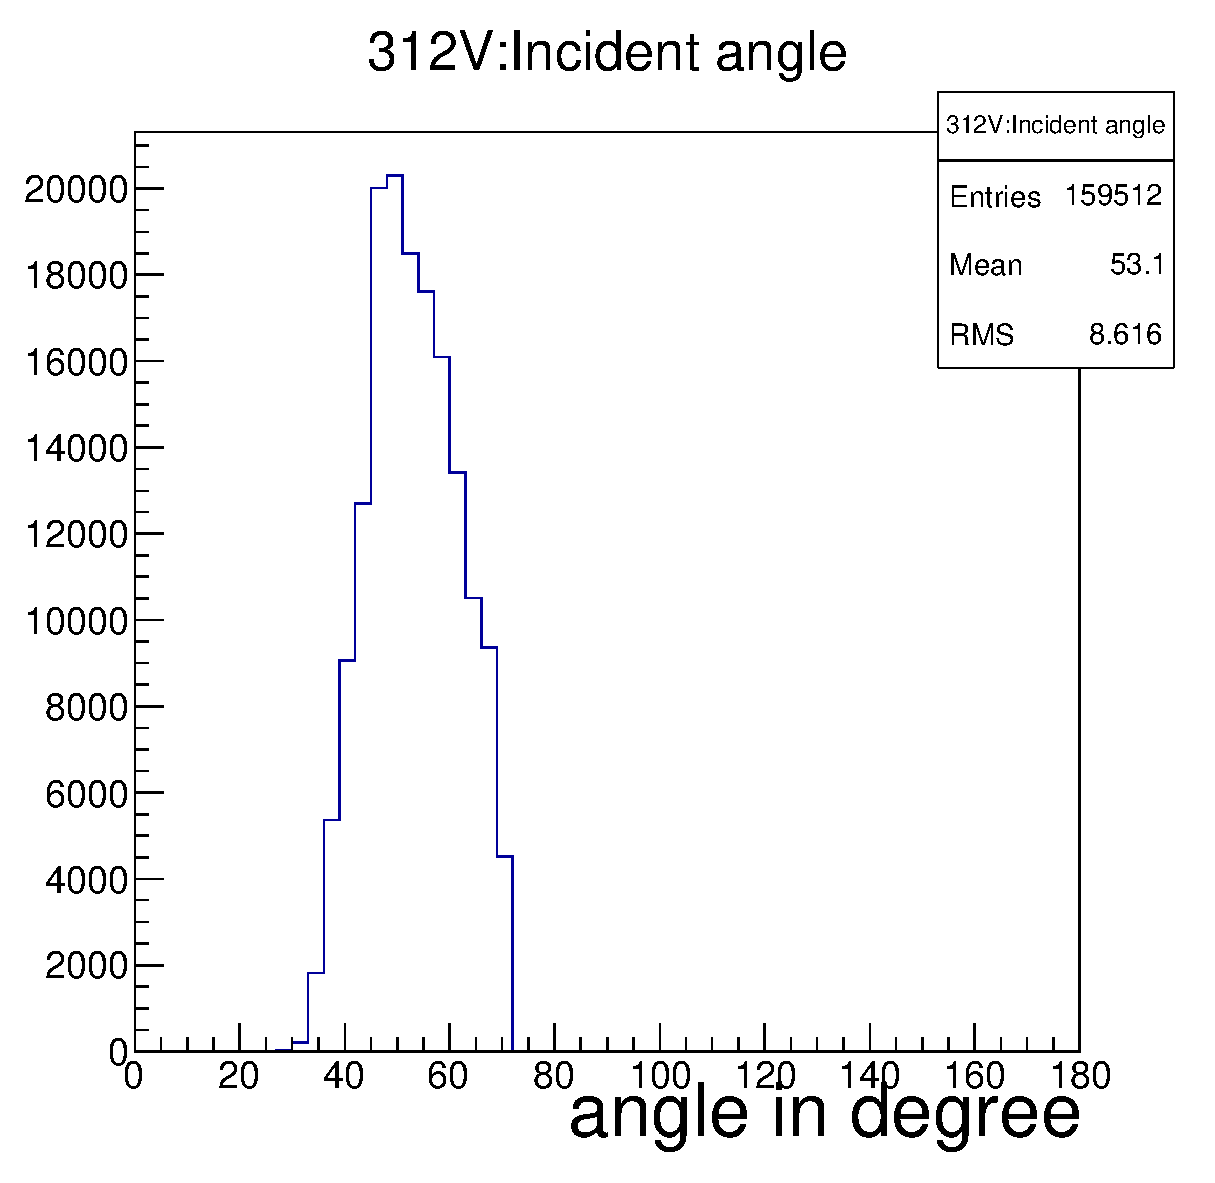
\includegraphics[width=.3\textwidth]{312V:incident_angle.eps}	
			\caption{Incident angle of the tracks}	
			\label{fig2}	
		\end{figure}
	\end{multicols}
	
	\begin{multicols}{4}
		
		\begin{figure}[H]
			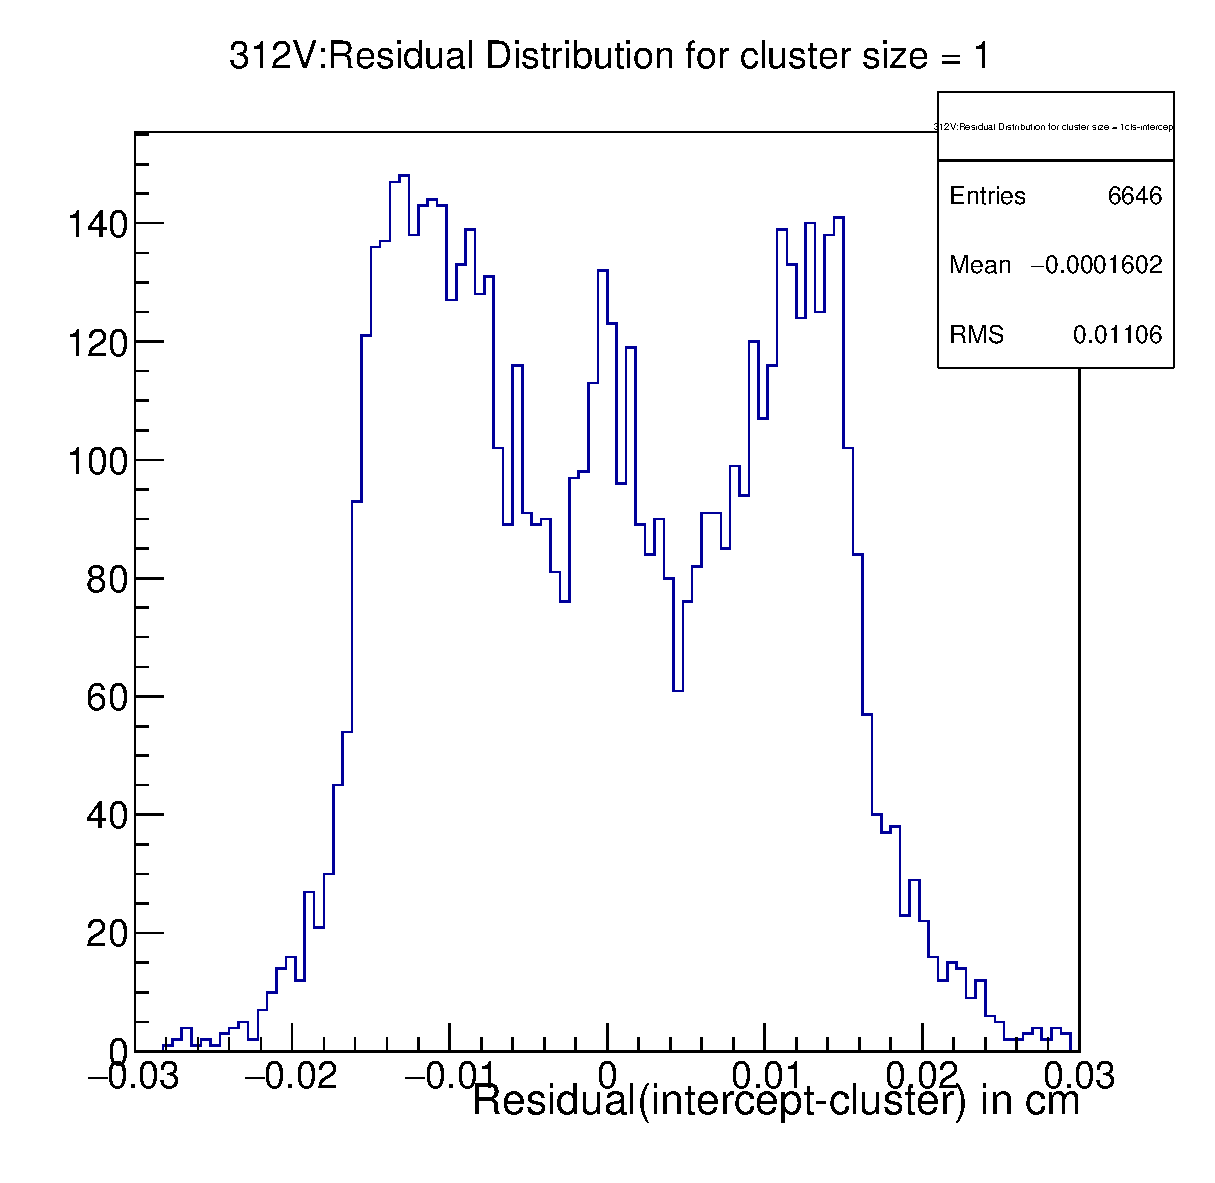
\includegraphics[width=.2\textwidth]{312V:clssize1.eps}	
			\caption{Residual distribution:Cluster size=1}	
			\label{fig1}	
		\end{figure}
		\begin{figure}[H]
			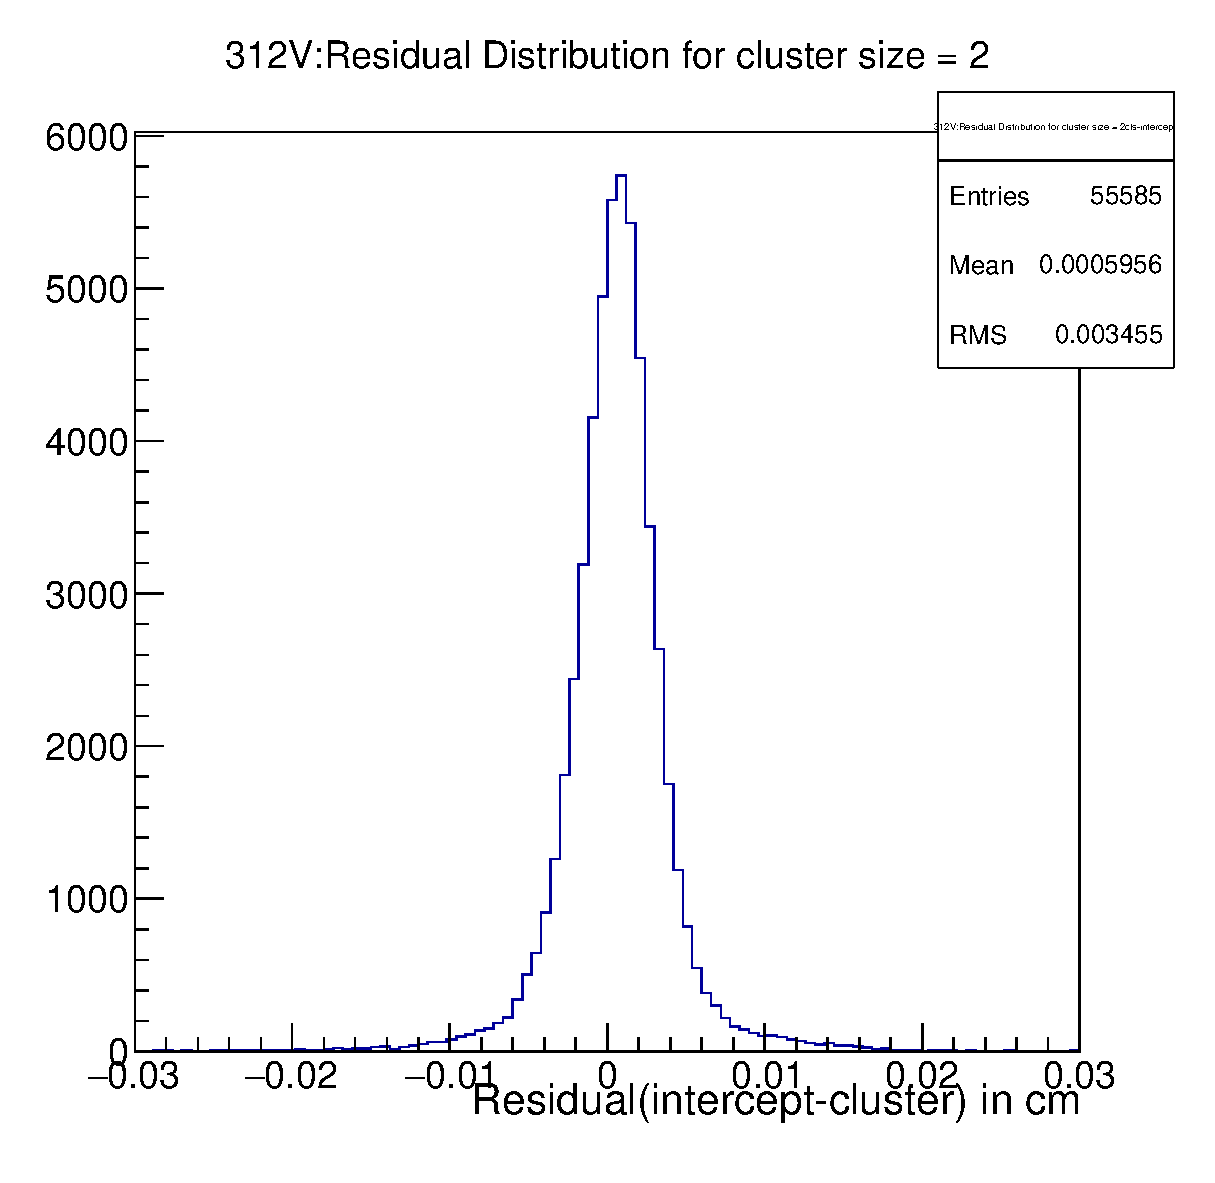
\includegraphics[width=.2\textwidth]{312V:clssize2.eps}	
			\caption{Residual distribution:Cluster size=2}	
			\label{fig2}	
		\end{figure}
		\begin{figure}[H]
			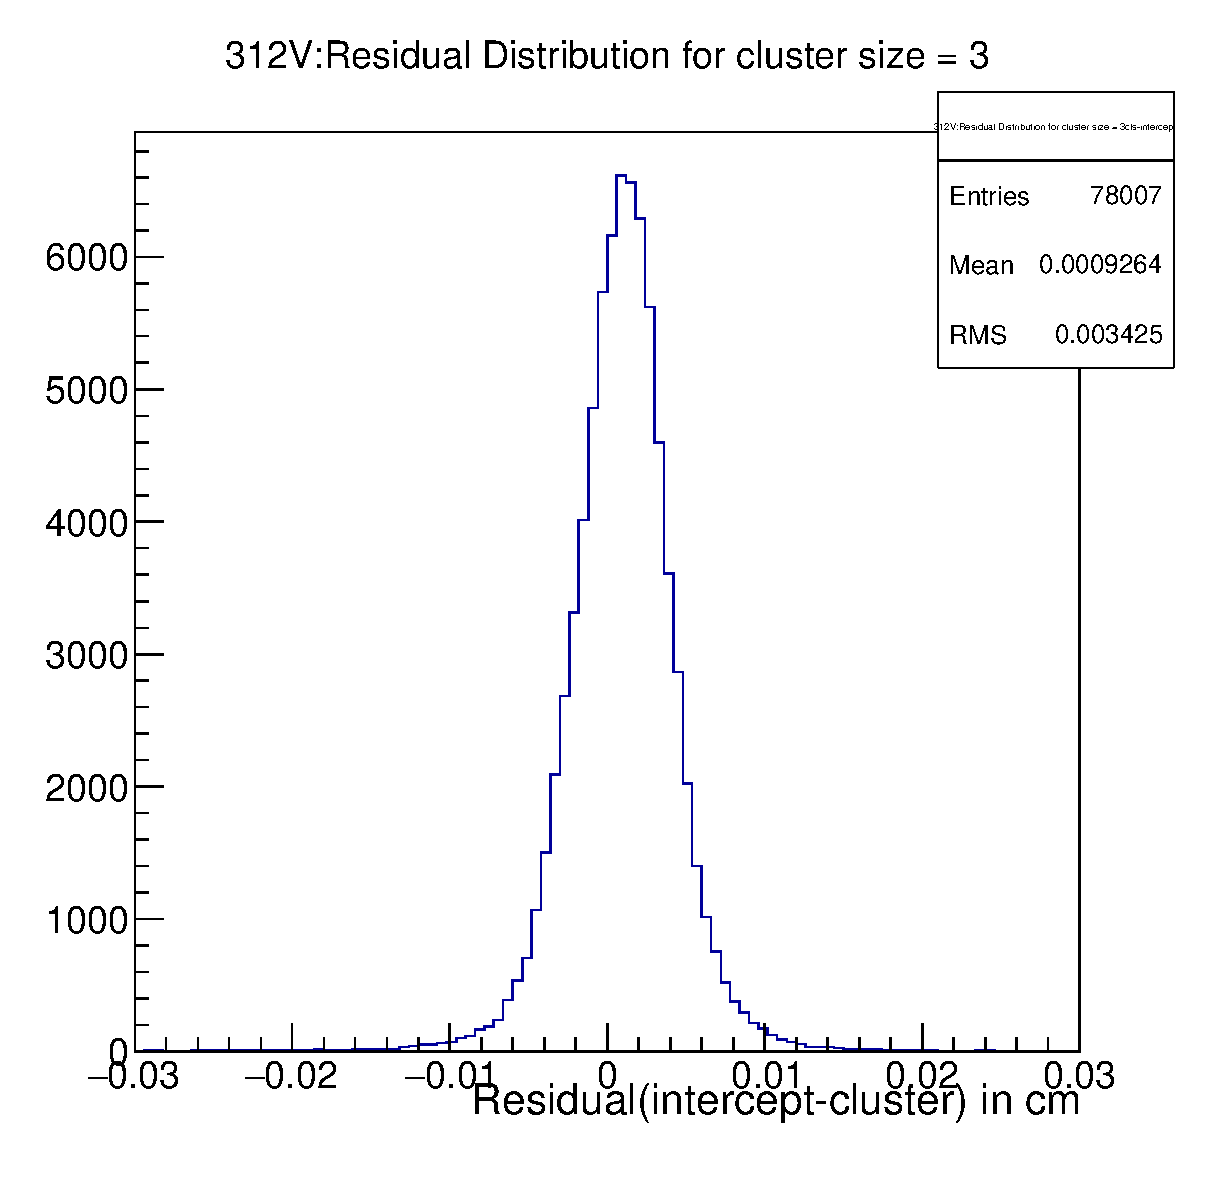
\includegraphics[width=.2\textwidth]{312V:clssize3.eps}	
			\caption{Residual distribution:Cluster size=3}	
			\label{fig2}	
		\end{figure}
		\begin{figure}[H]
			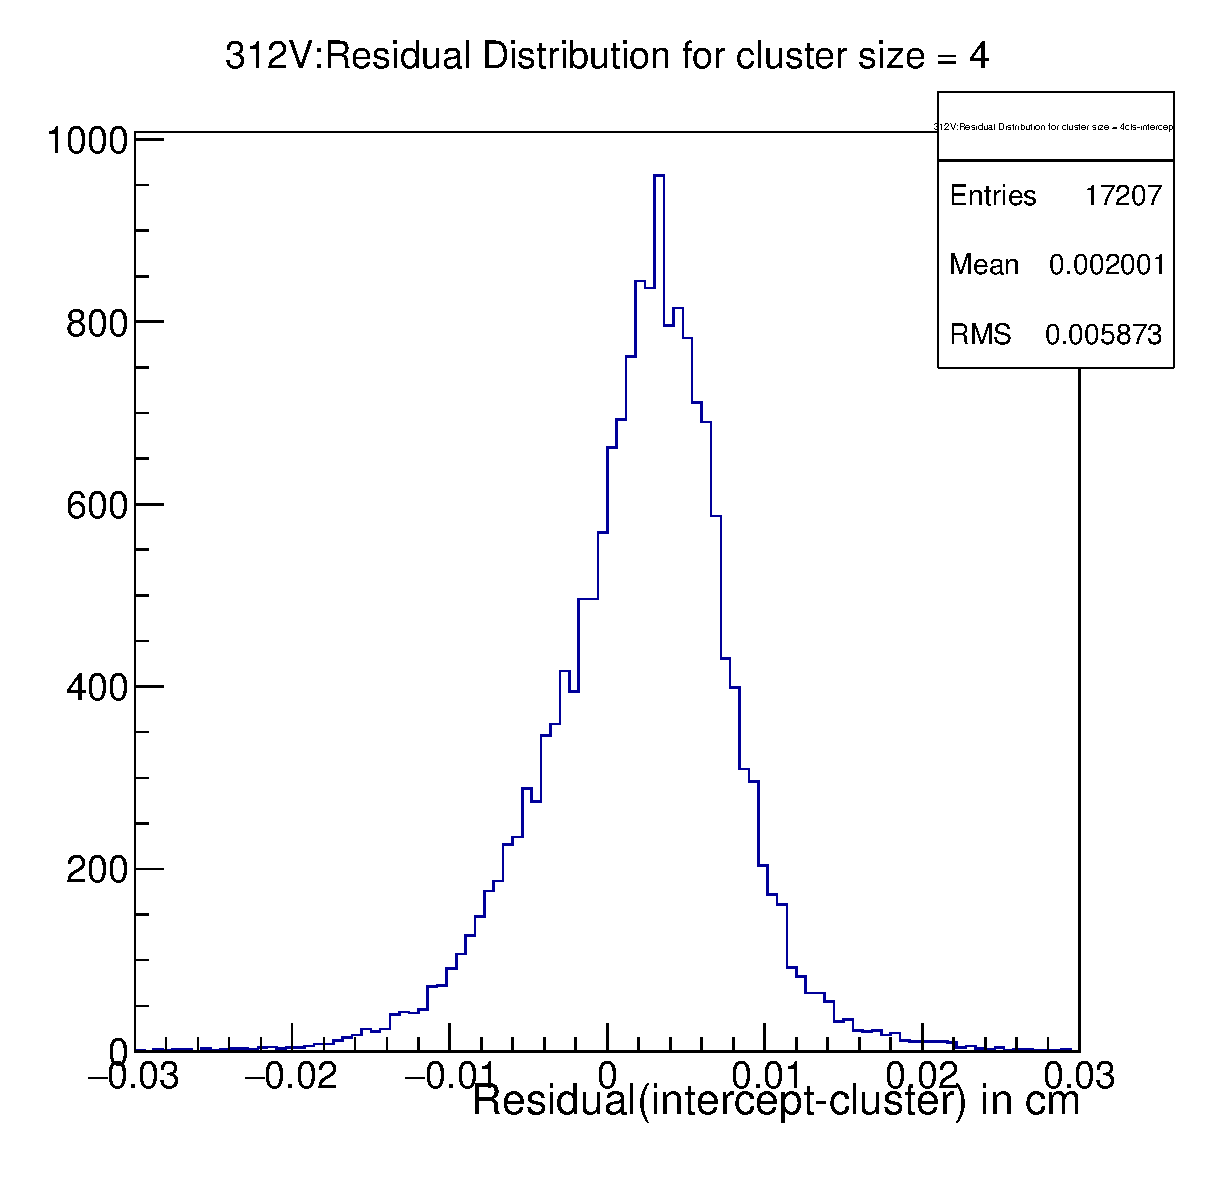
\includegraphics[width=.2\textwidth]{312V:clssize4.eps}	
			\caption{Residual distribution:Cluster size=4}	
			\label{fig2}	
		\end{figure}
	\end{multicols}
		\begin{figure}[H]
			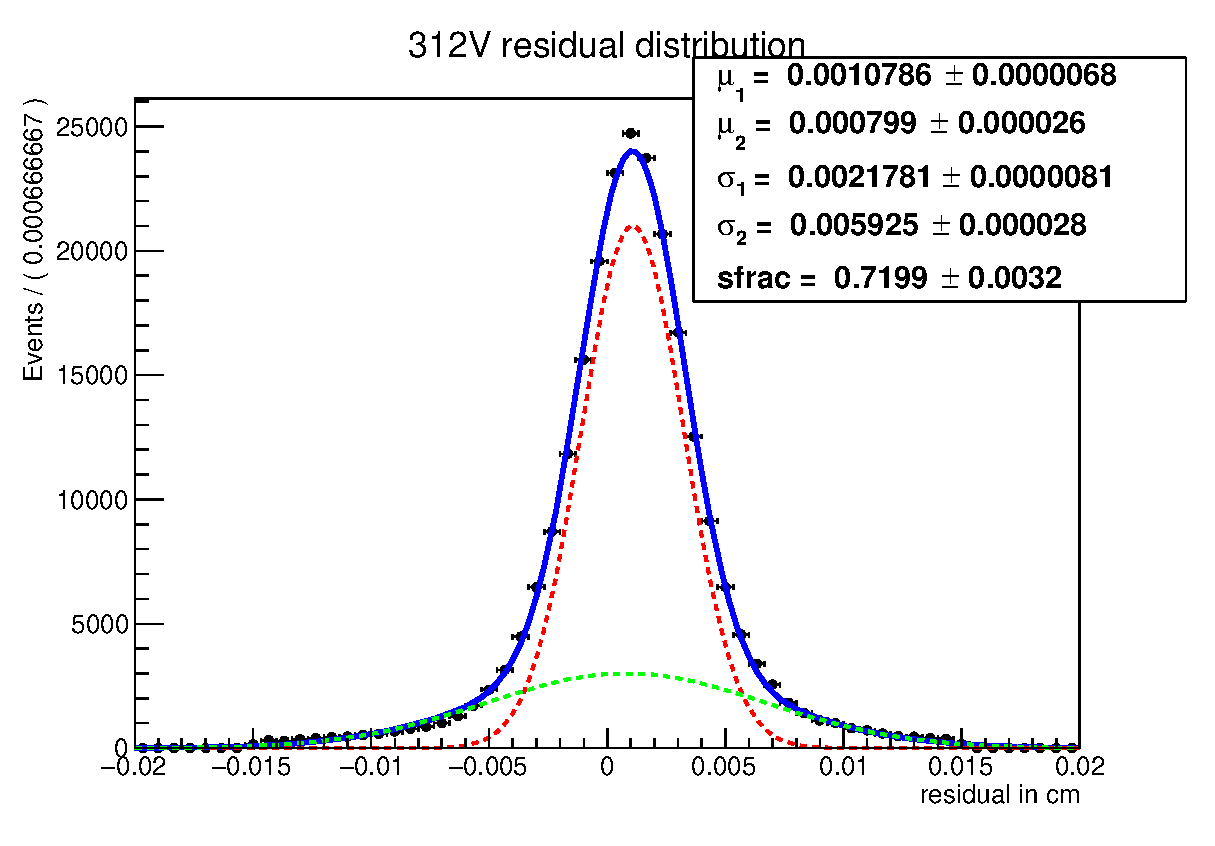
\includegraphics[width=.4\textwidth]{312V:fitted_residual.eps}	
			\caption{Residual distribution fitted with two Gaussian with different $\mu$ and $\sigma$ }	
			\label{fig2}	
		\end{figure}
	\pagebreak
	   \subsection{Layer4}
	   \subsubsection{Sensor1 V\_side}
	   \begin{multicols}{3}
	   	
	   	\begin{figure}[H]
	   		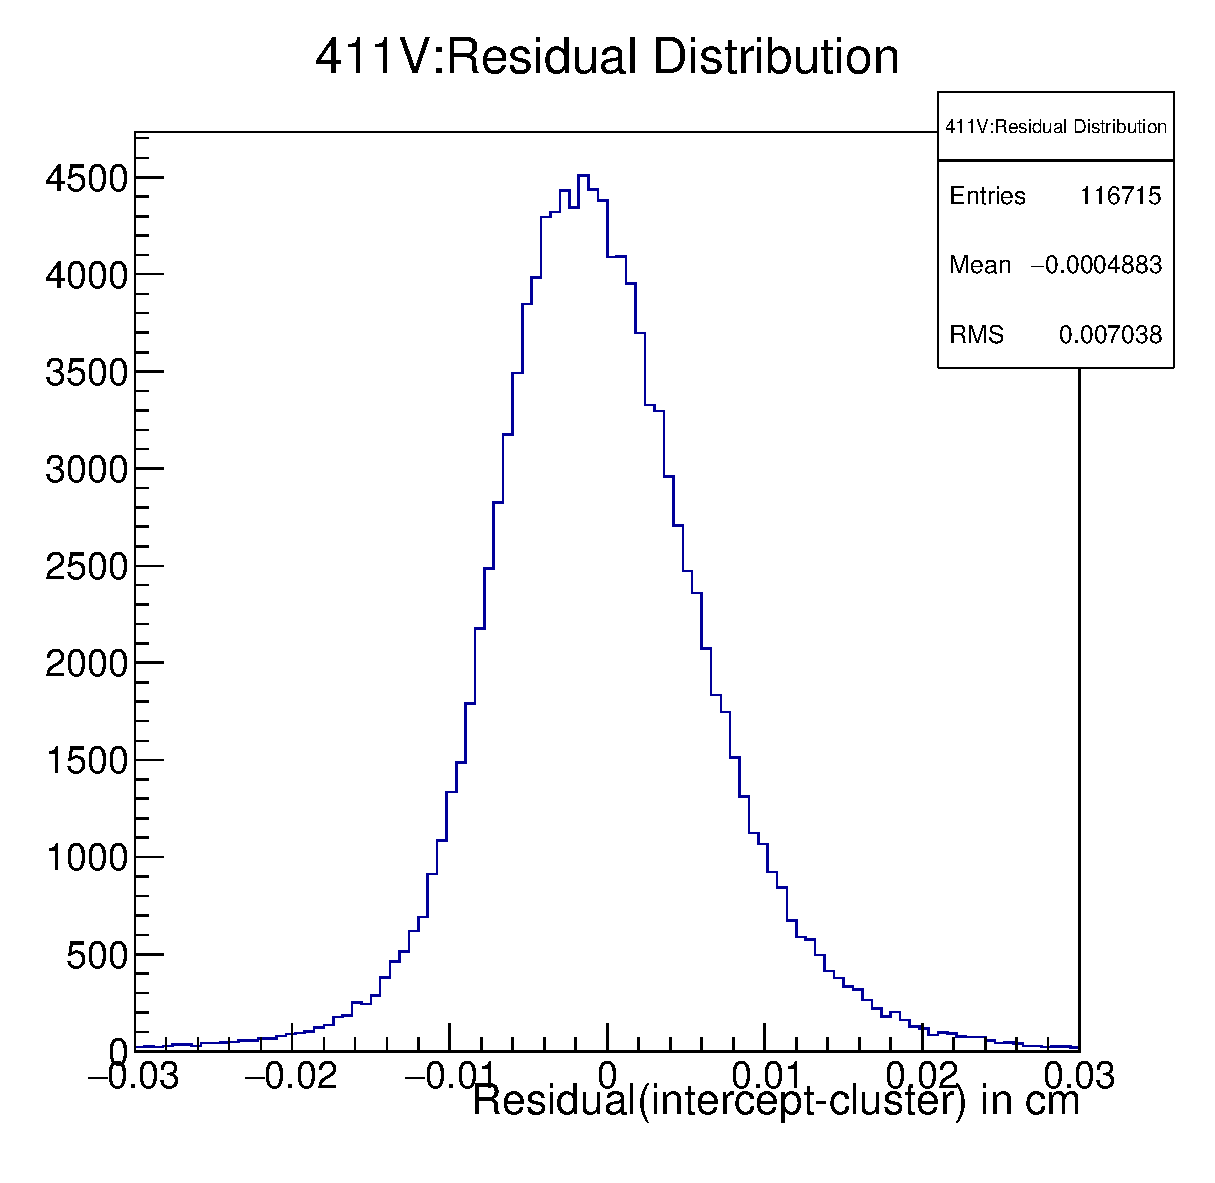
\includegraphics[width=.3\textwidth]{411V:residualplot.eps}	
	   		\caption{Residual distribution}	
	   		\label{fig1}	
	   	\end{figure}
	   	\begin{figure}[H]
	   		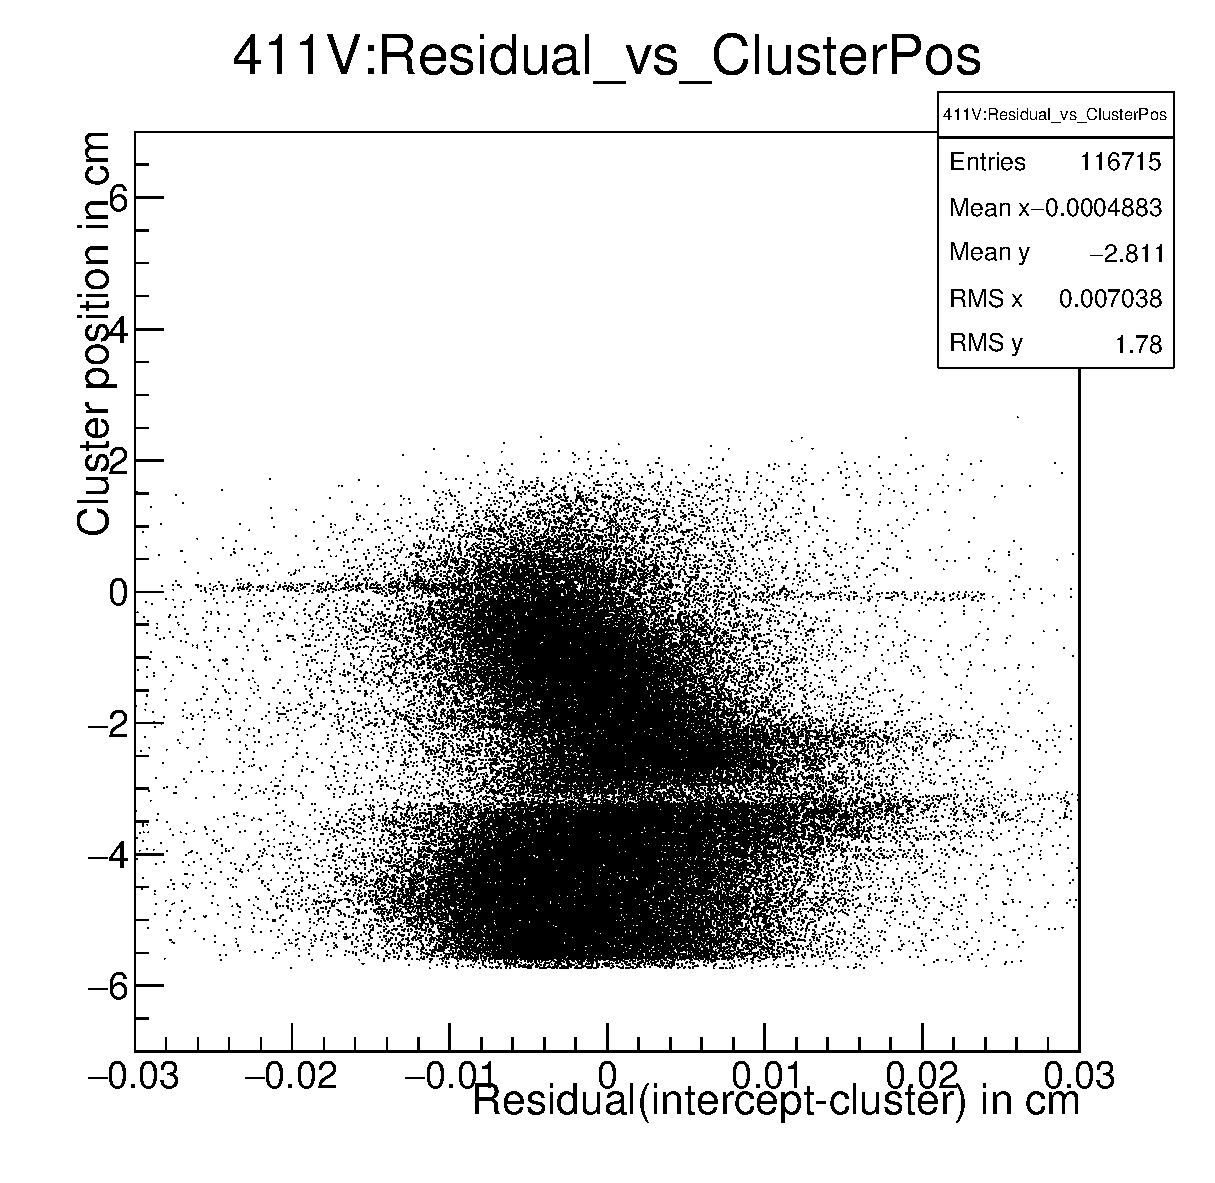
\includegraphics[width=.3\textwidth]{411V:residual_vs_clusterpos.eps}	
	   		\caption{Cluster position vs Residual}	
	   		\label{fig2}	
	   	\end{figure}
	   	\begin{figure}[H]
	   		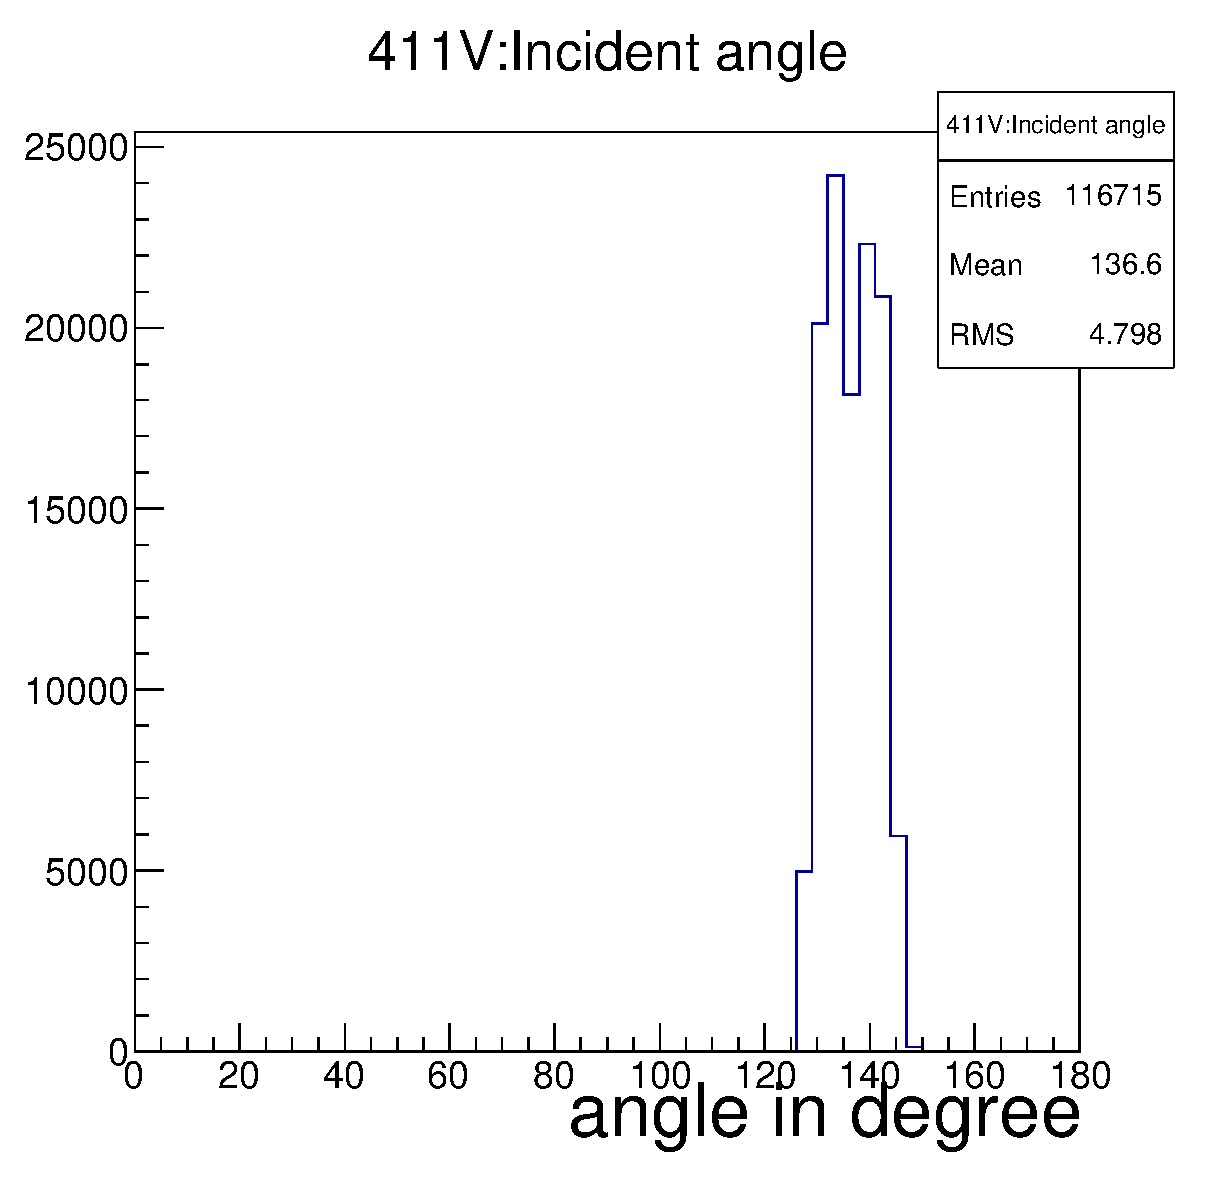
\includegraphics[width=.3\textwidth]{411V:incident_angle.eps}	
	   		\caption{Incident angle of the tracks}	
	   		\label{fig2}	
	   	\end{figure}
	   \end{multicols}
	   
	   \begin{multicols}{4}
	   	
	   	\begin{figure}[H]
	   		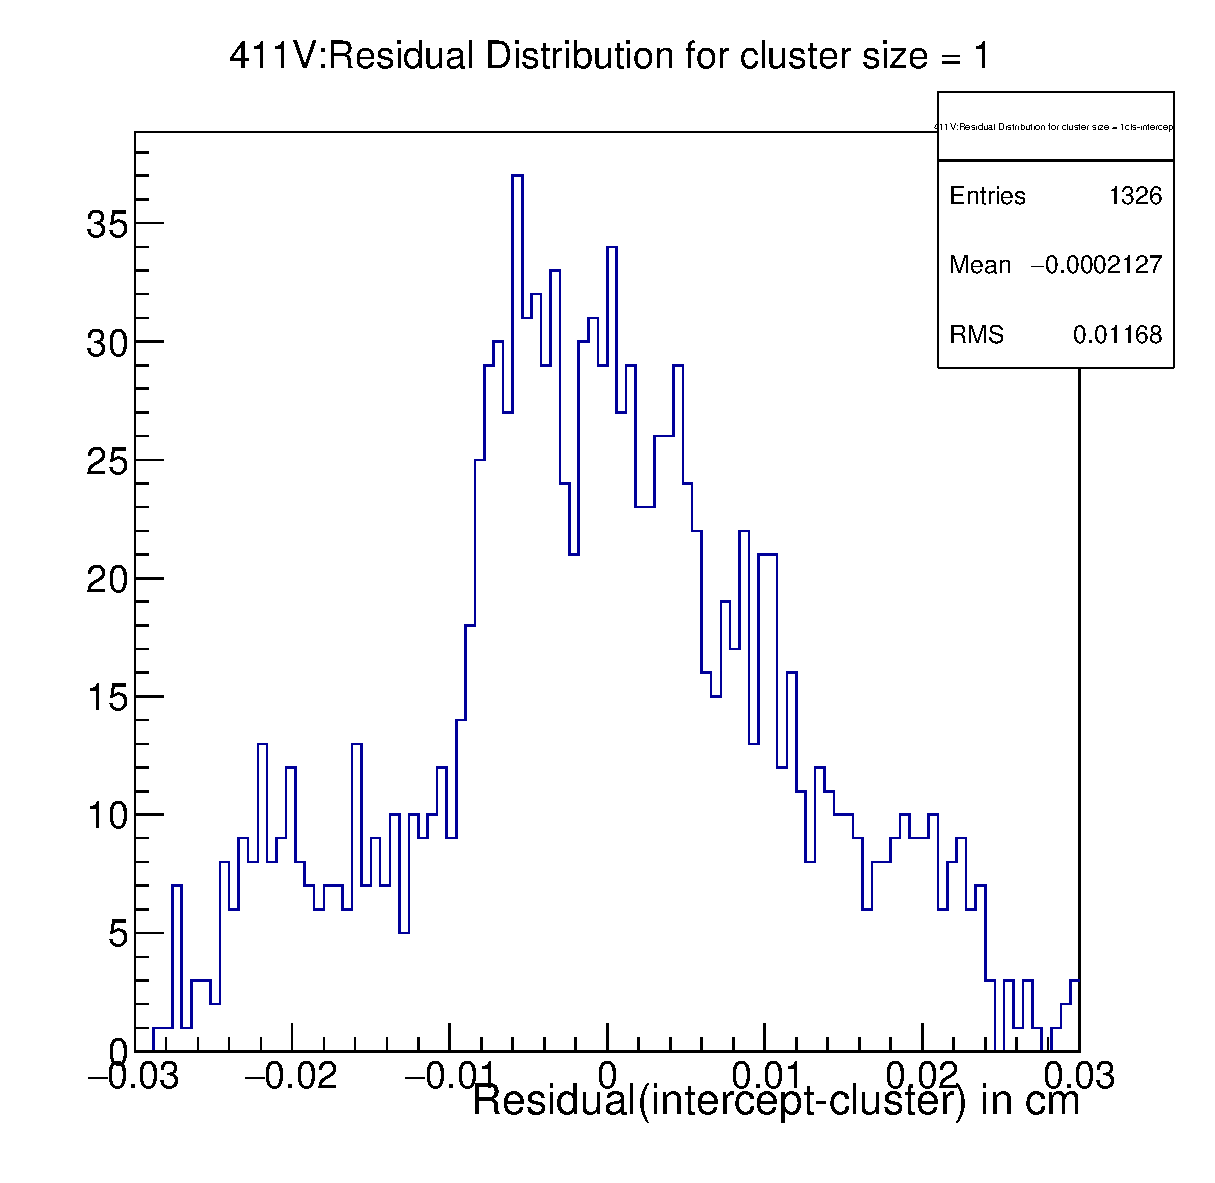
\includegraphics[width=.2\textwidth]{411V:clssize1.eps}	
	   		\caption{Residual distribution:Cluster size=1}	
	   		\label{fig1}	
	   	\end{figure}
	   	\begin{figure}[H]
	   		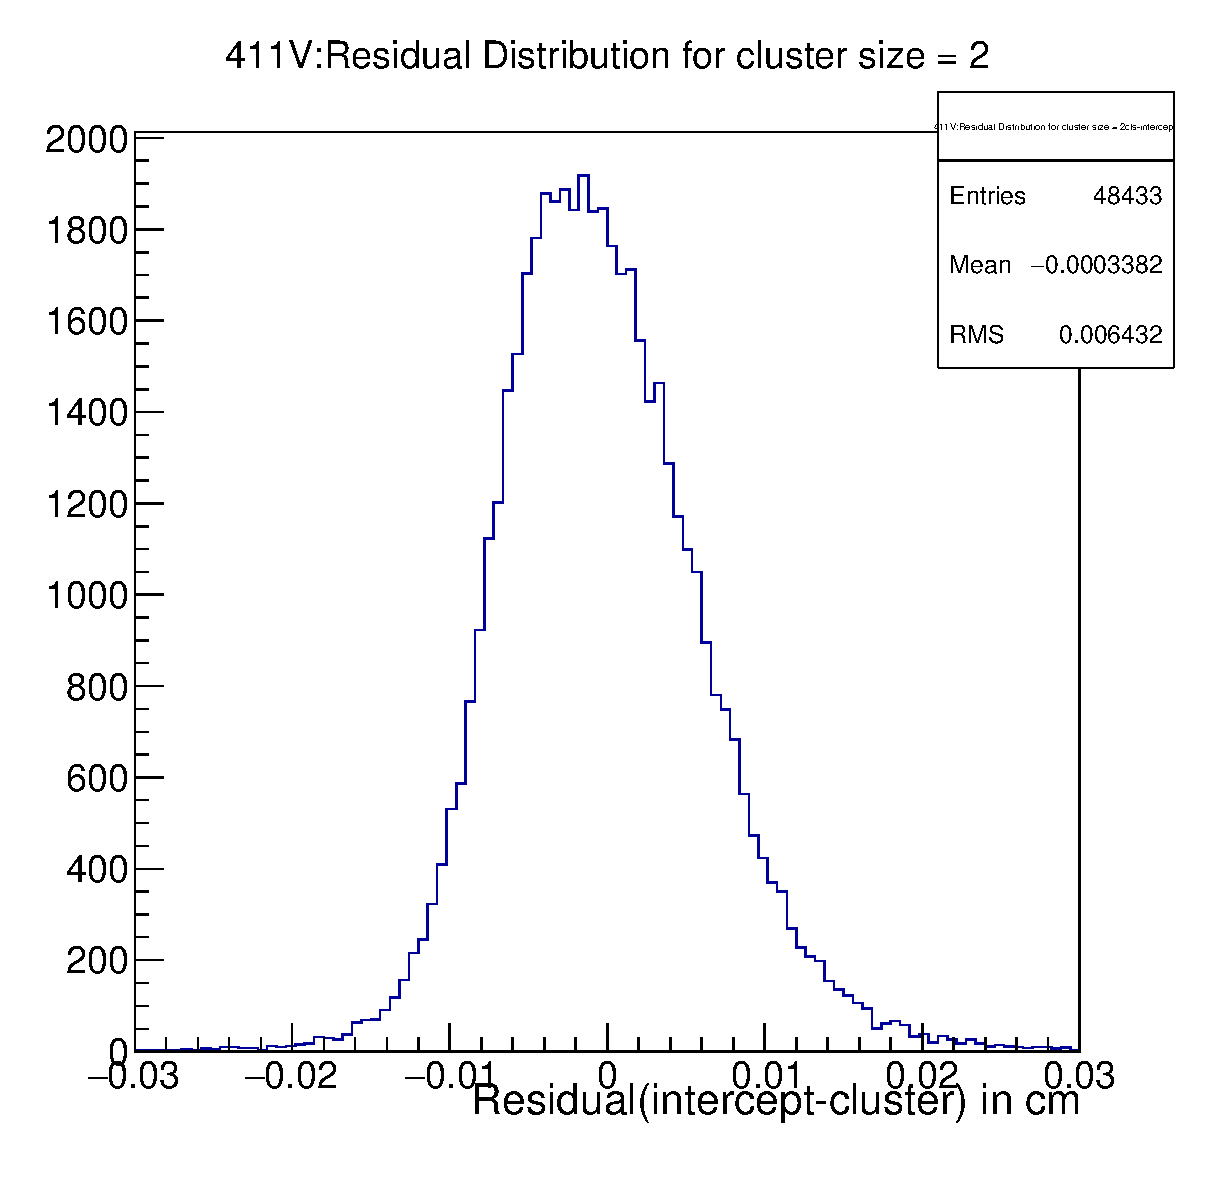
\includegraphics[width=.2\textwidth]{411V:clssize2.eps}	
	   		\caption{Residual distribution:Cluster size=2}	
	   		\label{fig2}	
	   	\end{figure}
	   	\begin{figure}[H]
	   		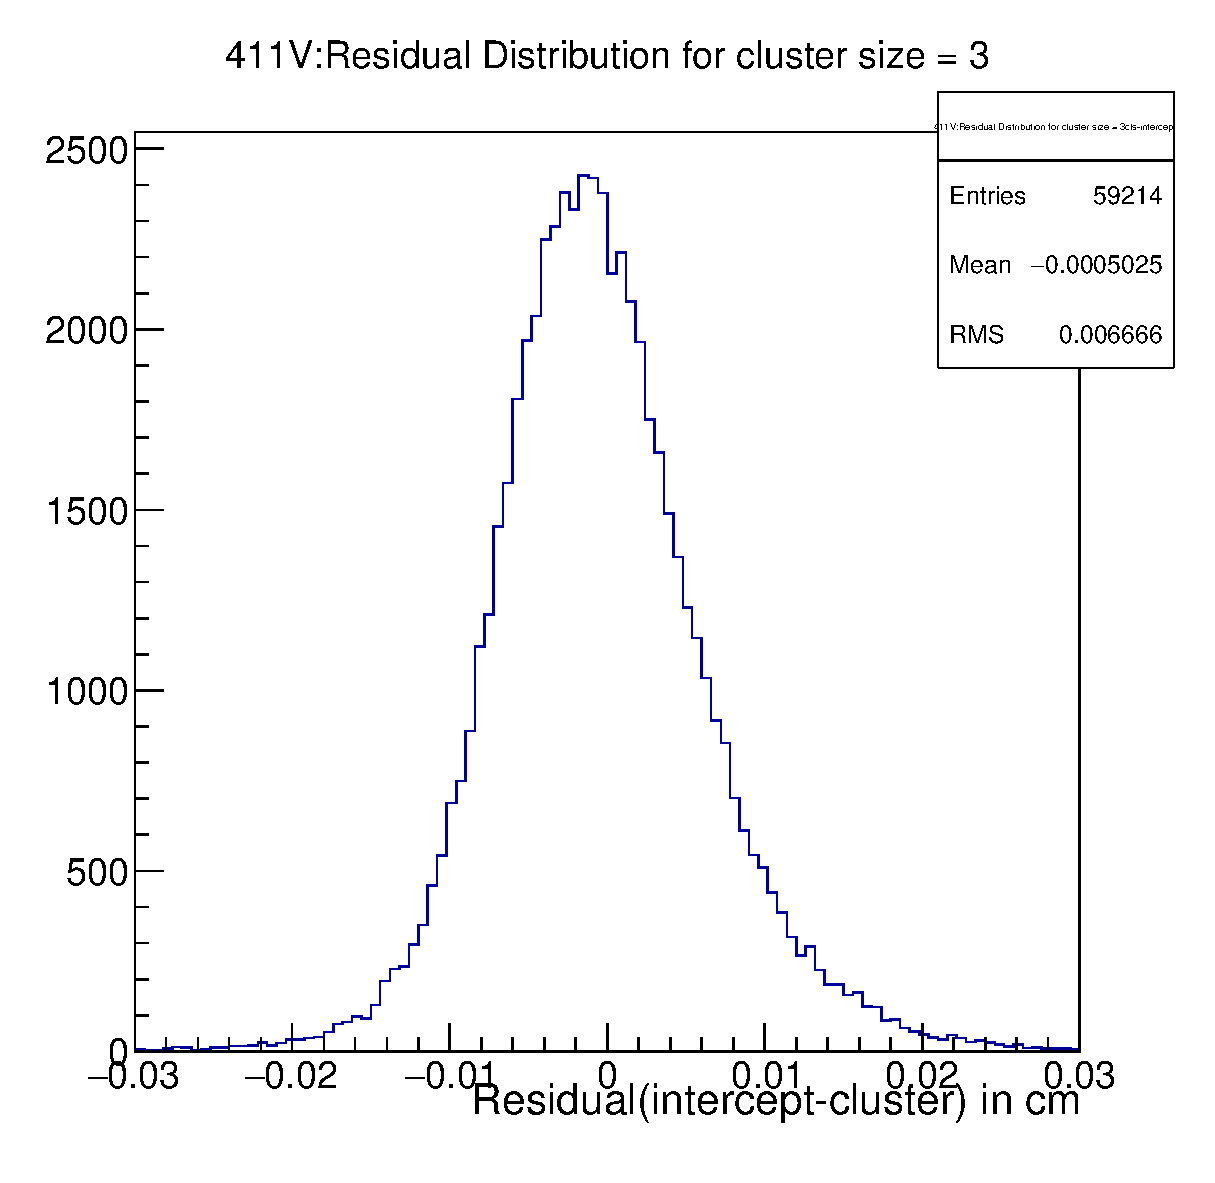
\includegraphics[width=.2\textwidth]{411V:clssize3.eps}	
	   		\caption{Residual distribution:Cluster size=3}	
	   		\label{fig2}	
	   	\end{figure}
	   	\begin{figure}[H]
	   		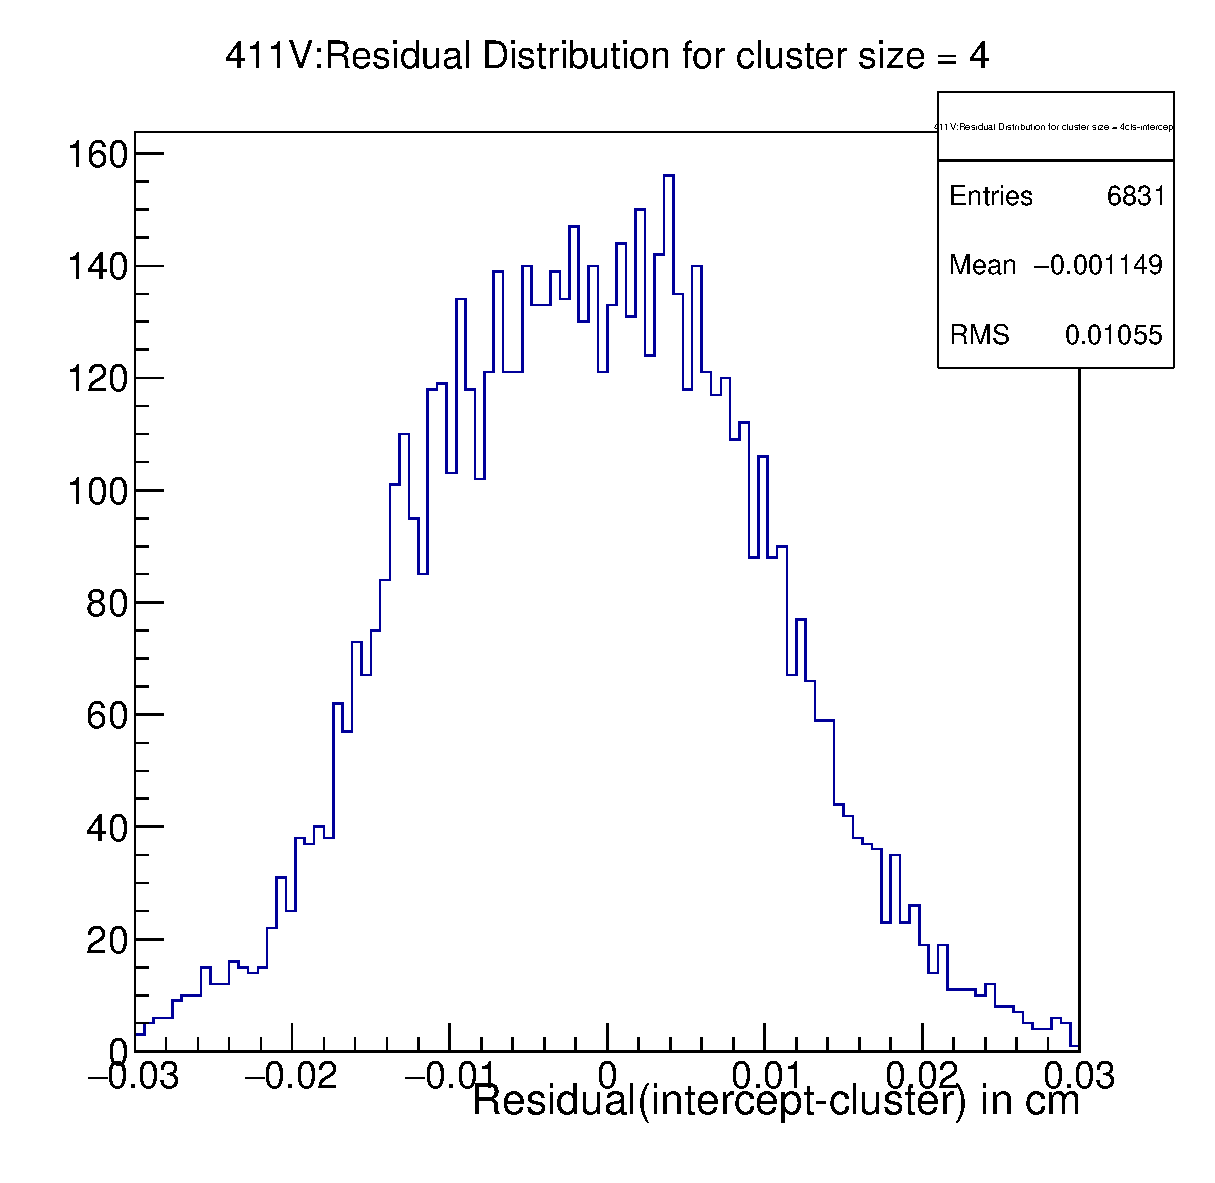
\includegraphics[width=.2\textwidth]{411V:clssize4.eps}	
	   		\caption{Residual distribution:Cluster size=4}	
	   		\label{fig2}	
	   	\end{figure}
	   \end{multicols}
	   	\begin{figure}[H]
	   		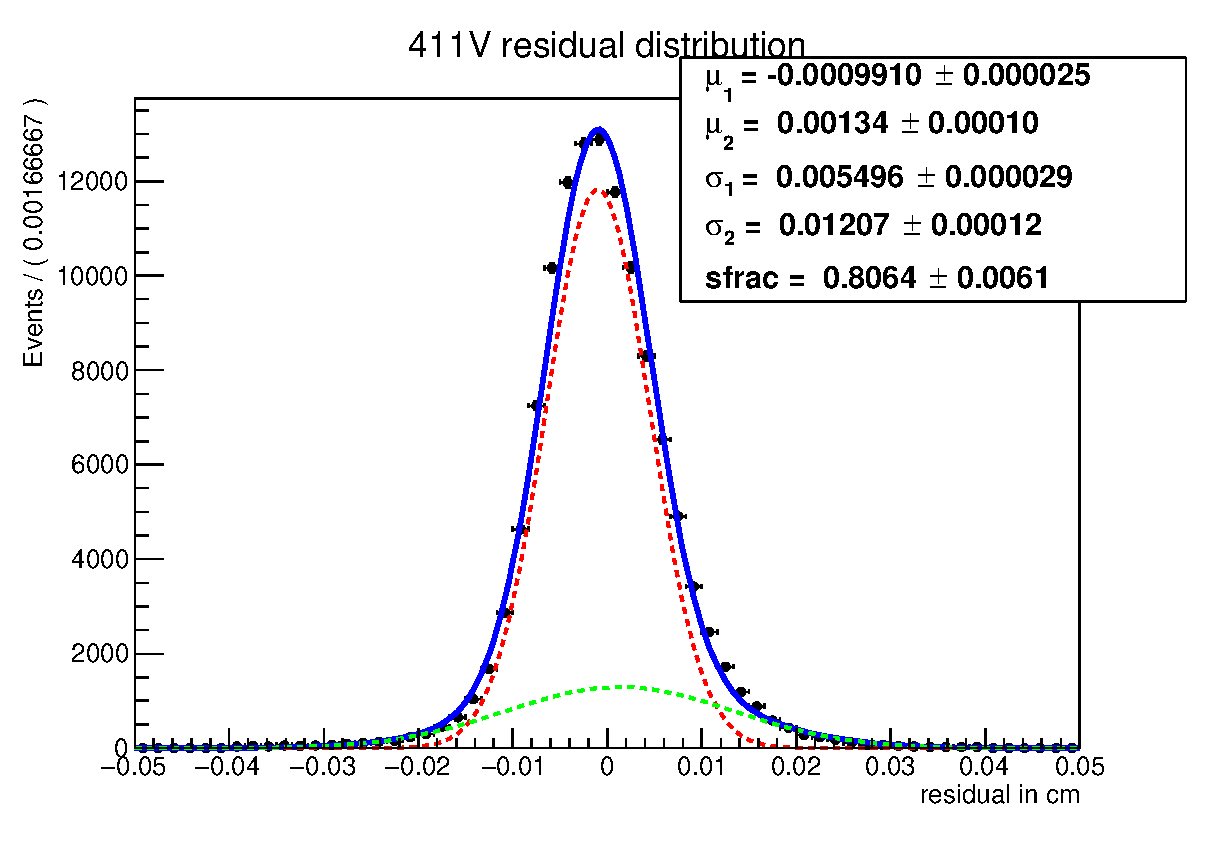
\includegraphics[width=.4\textwidth]{411V:fitted_residual.eps}	
	   		\caption{Residual distribution fitted with two Gaussian with different $\mu$ and $\sigma$ }	
	   		\label{fig2}	
	   	\end{figure}
	   \pagebreak
		\subsubsection{Sensor:2 U\_side}
		\begin{multicols}{3}
			
			\begin{figure}[H]
				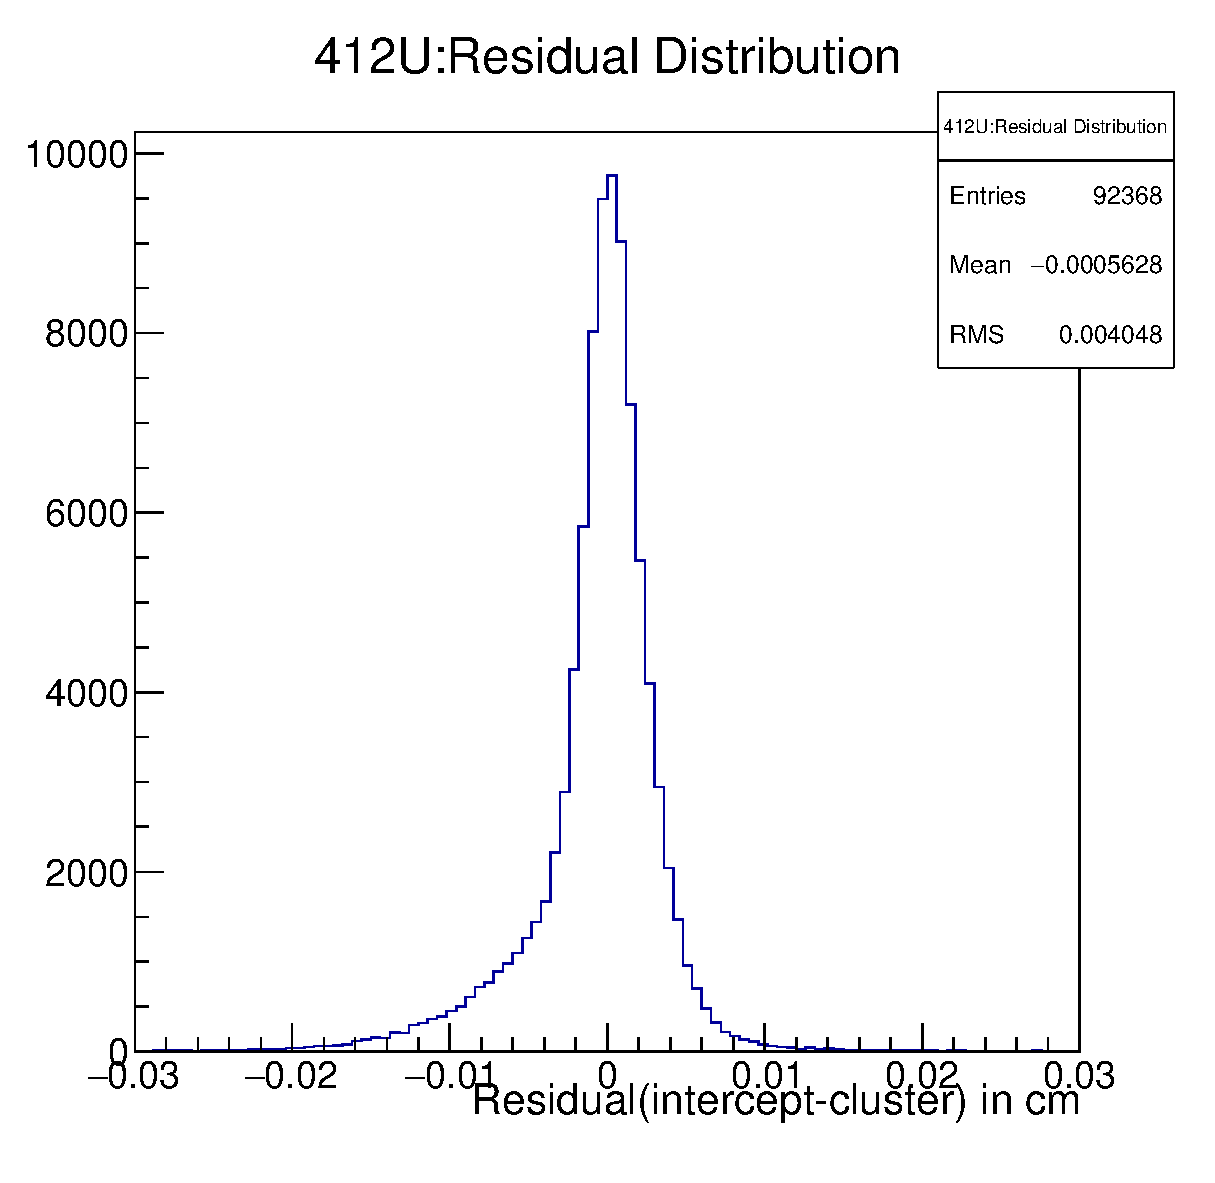
\includegraphics[width=.3\textwidth]{412U:residualplot.eps}	
				\caption{Residual distribution}	
				\label{fig1}	
			\end{figure}
			\begin{figure}[H]
				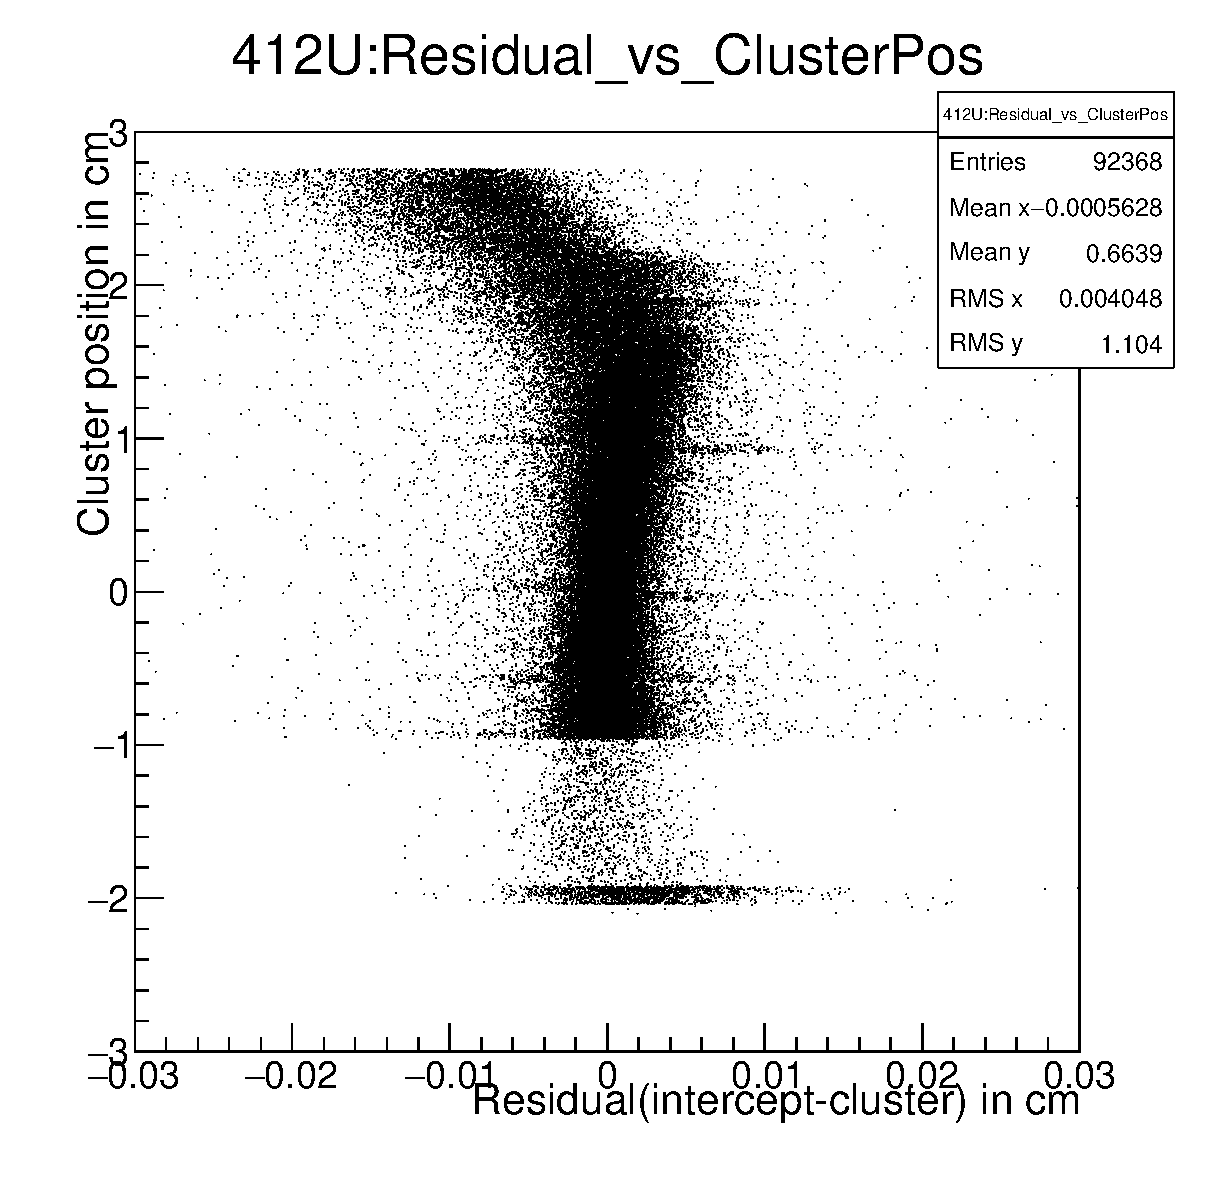
\includegraphics[width=.3\textwidth]{412U:residual_vs_clusterpos.eps}	
				\caption{Cluster position vs Residual}	
				\label{fig2}	
			\end{figure}
			\begin{figure}[H]
				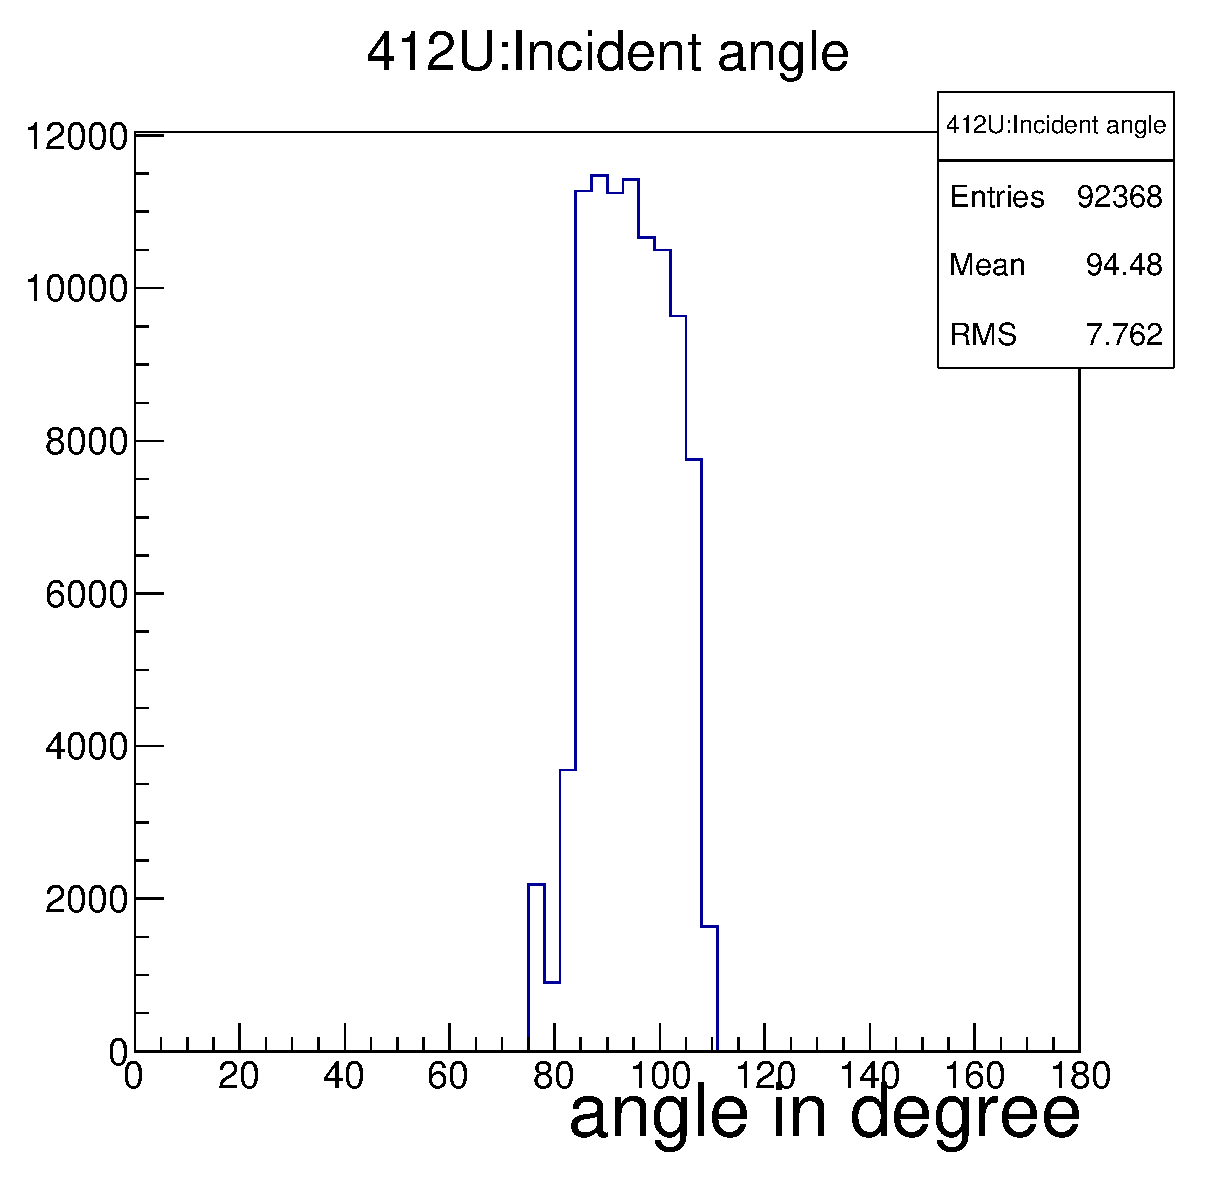
\includegraphics[width=.3\textwidth]{412U:incident_angle.eps}	
				\caption{Incident angle of the tracks}	
				\label{fig2}	
			\end{figure}
		\end{multicols}
		
		\begin{multicols}{4}
			
			\begin{figure}[H]
				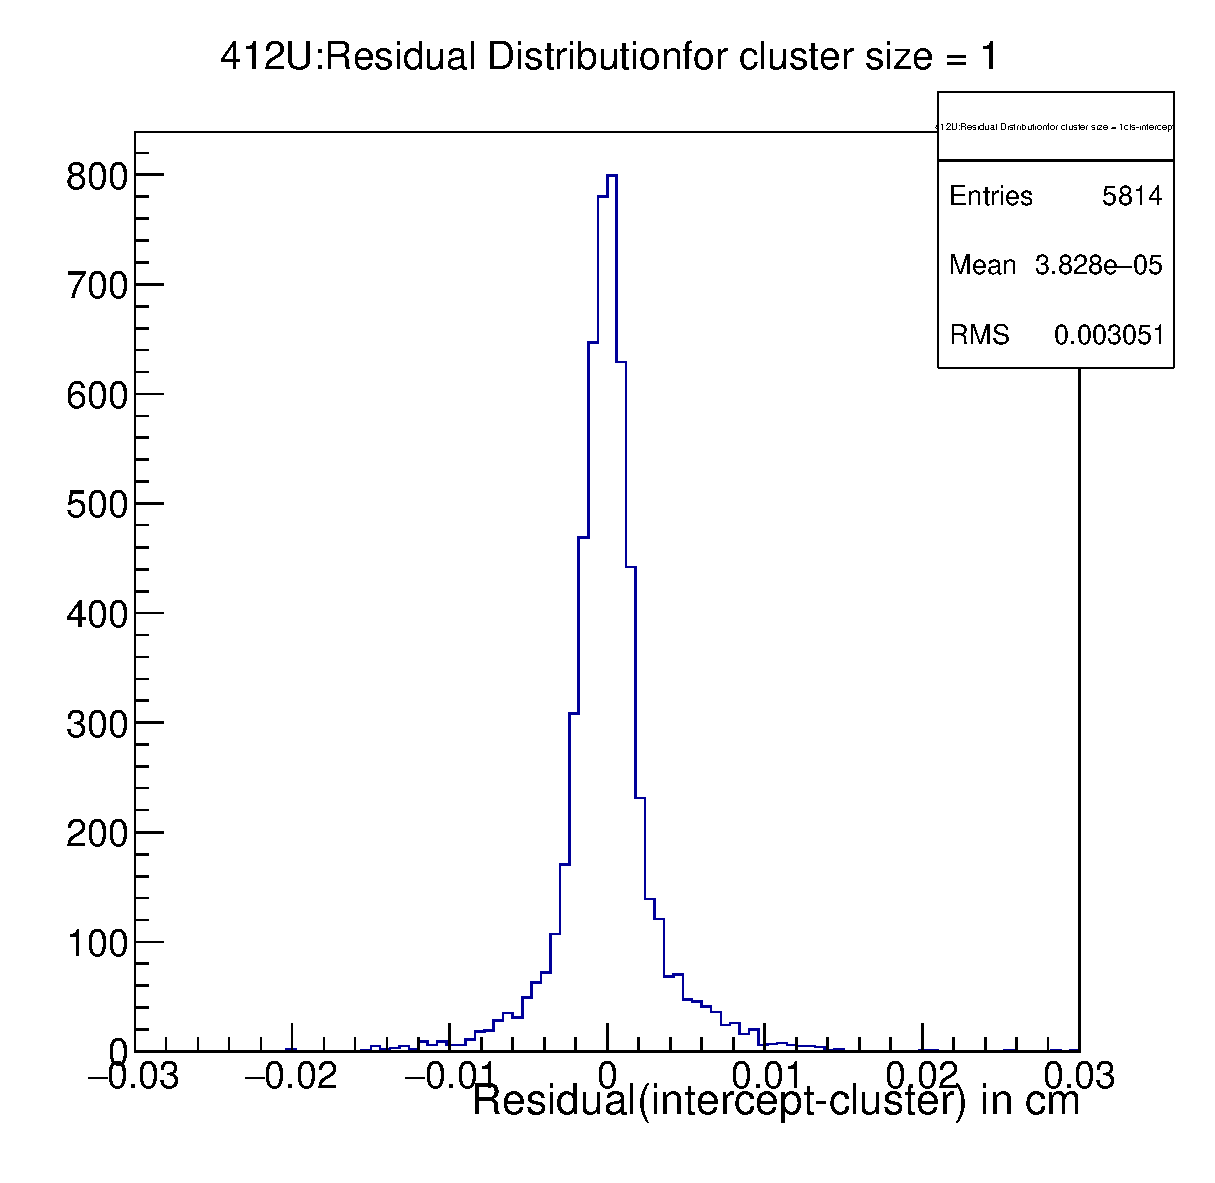
\includegraphics[width=.2\textwidth]{412U:clssize1.eps}	
				\caption{Residual distribution:Cluster size=1}	
				\label{fig1}	
			\end{figure}
			\begin{figure}[H]
				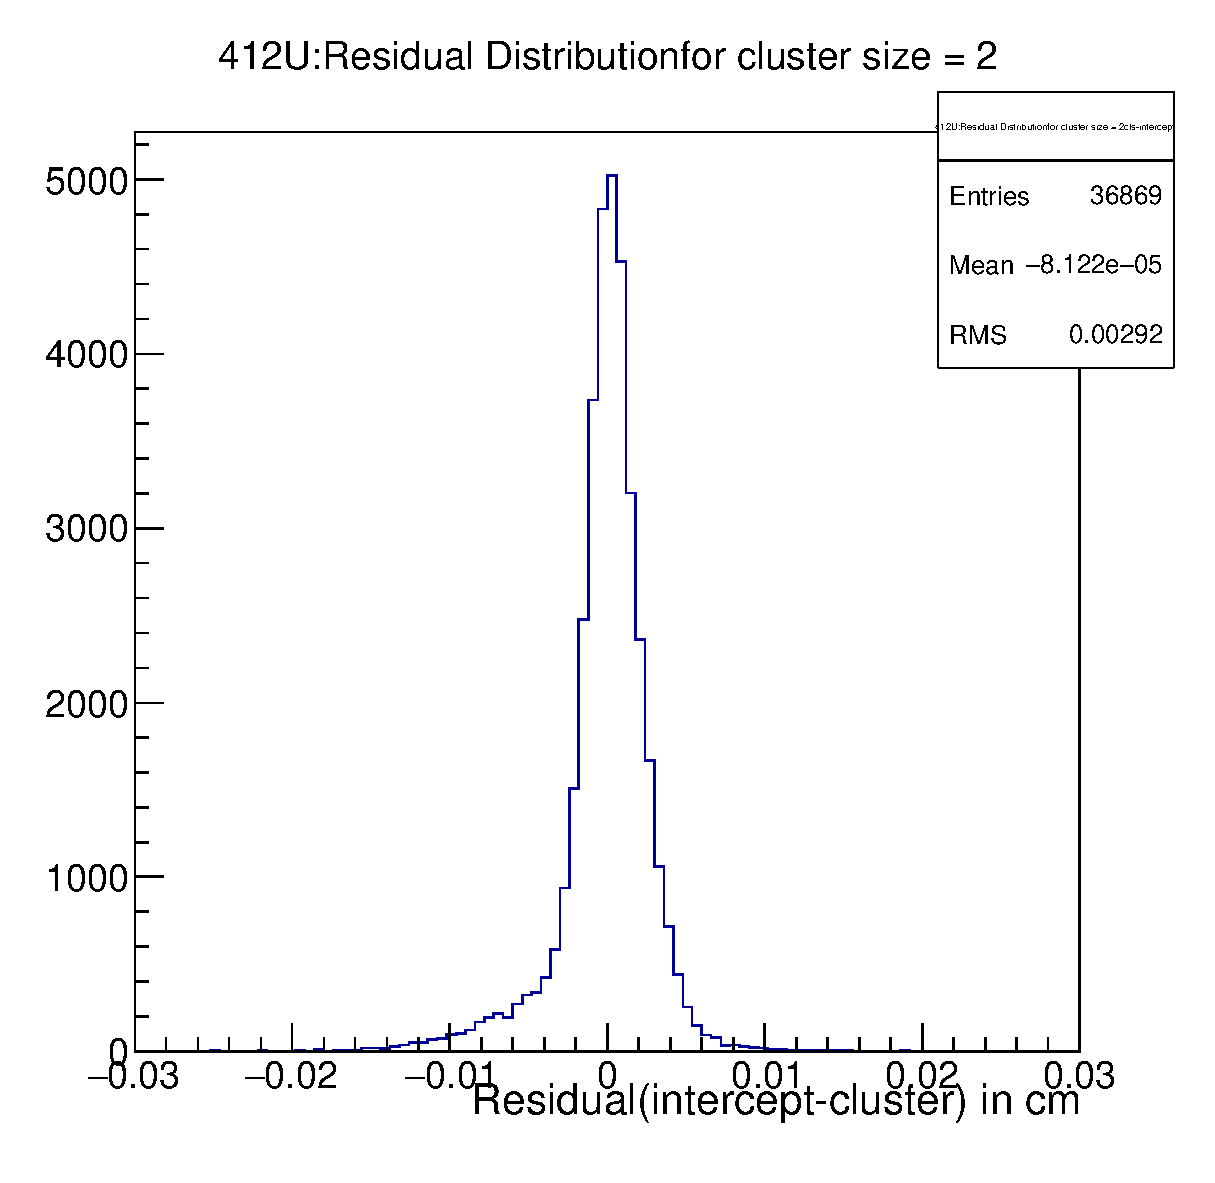
\includegraphics[width=.2\textwidth]{412U:clssize2.eps}	
				\caption{Residual distribution:Cluster size=2}	
				\label{fig2}	
			\end{figure}
			\begin{figure}[H]
				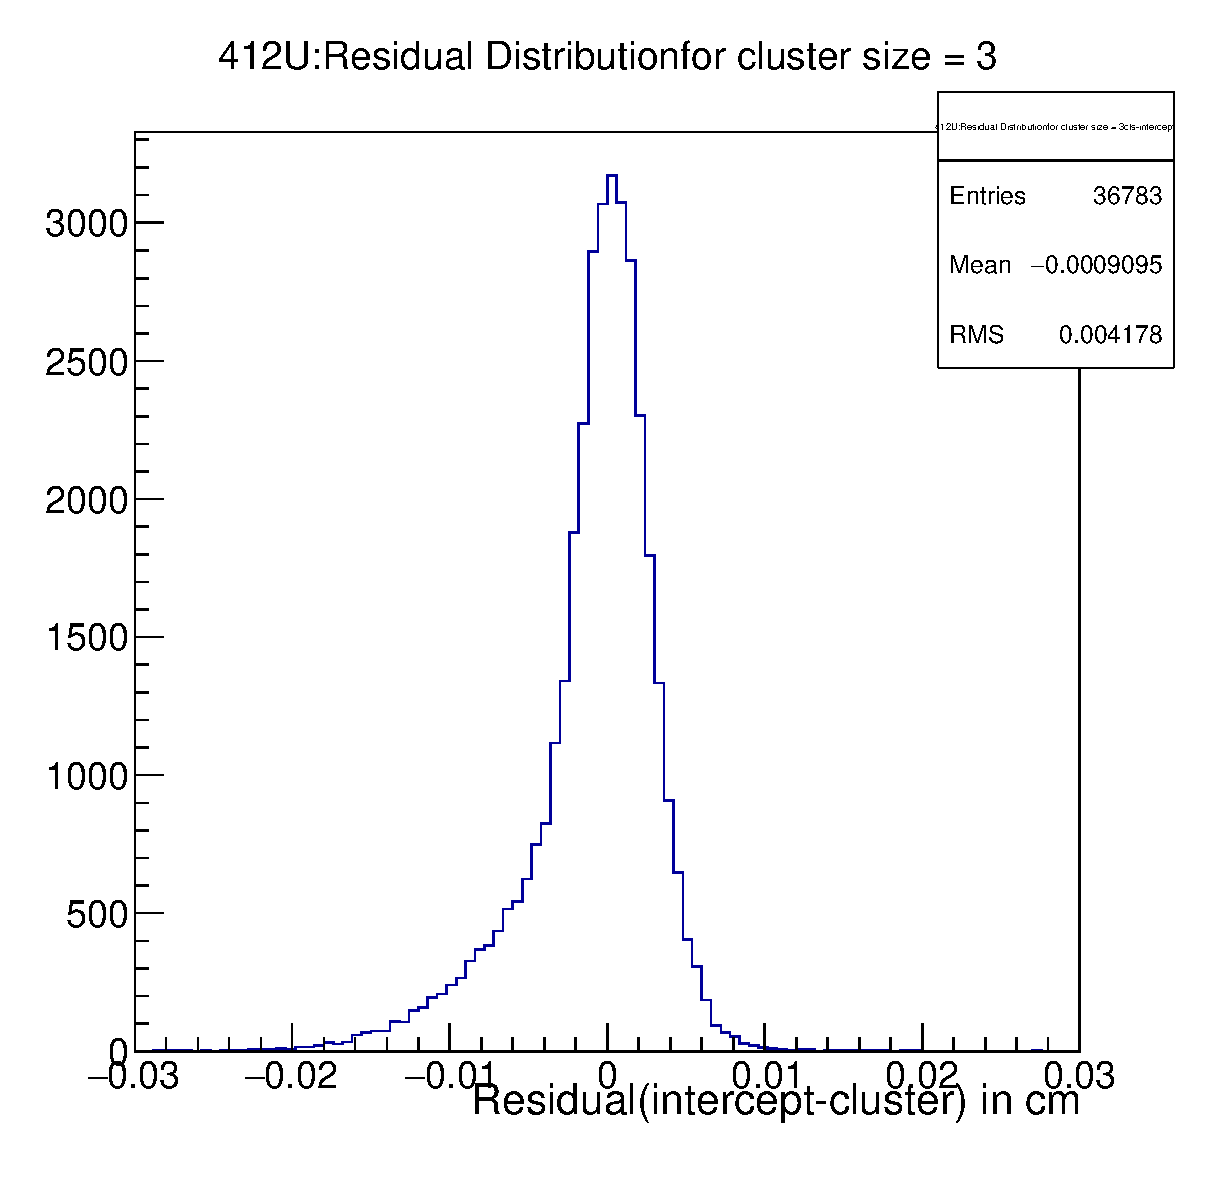
\includegraphics[width=.2\textwidth]{412U:clssize3.eps}	
				\caption{Residual distribution:Cluster size=3}	
				\label{fig2}	
			\end{figure}
			\begin{figure}[H]
				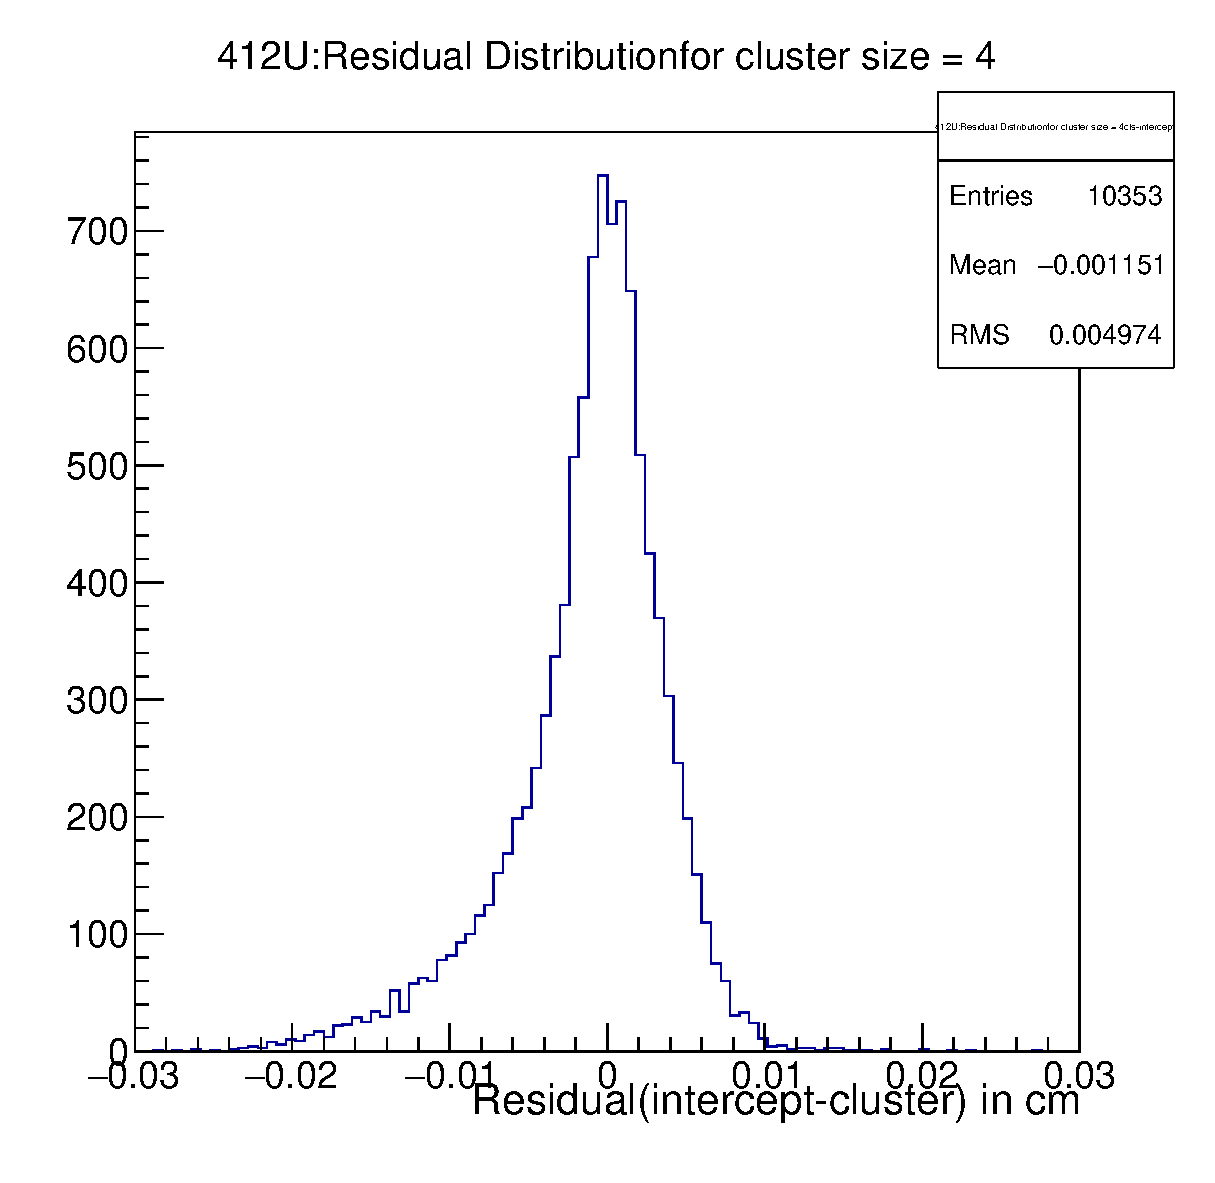
\includegraphics[width=.2\textwidth]{412U:clssize4.eps}	
				\caption{Residual distribution:Cluster size=4}	
				\label{fig2}	
			\end{figure}
		\end{multicols}
			\begin{figure}[H]
				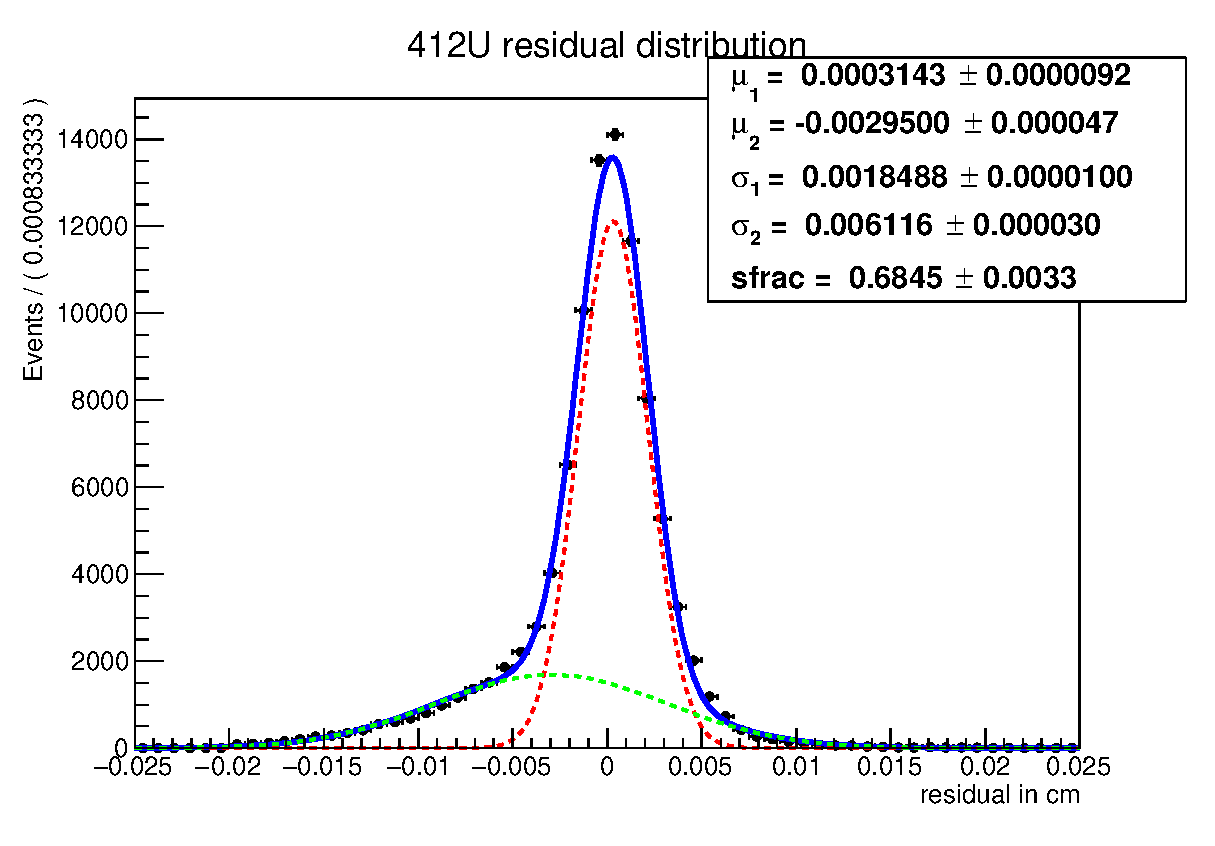
\includegraphics[width=.4\textwidth]{412U:fitted_residual.eps}	
				\caption{Residual distribution fitted with two Gaussian with different $\mu$ and $\sigma$ }	
				\label{fig2}	
			\end{figure}
		\pagebreak
		\subsubsection{Sensor:2 V\_side}
		\begin{multicols}{3}
			\begin{figure}[H]
				\includegraphics[width=.3\textwidth]{412V:residualplot.eps}	
				\caption{Residual distribution}	
				\label{fig1}	
			\end{figure}
			\begin{figure}[H]
				\includegraphics[width=.3\textwidth]{412V:residual_vs_clusterpos.eps}	
				\caption{Cluster position vs Residual}	
				\label{fig2}	
			\end{figure}
			\begin{figure}[H]
				\includegraphics[width=.3\textwidth]{412V:incident_angle.eps}	
				\caption{Incident angle of the tracks}	
				\label{fig2}	
			\end{figure}
		\end{multicols}
		
		\begin{multicols}{4}
			
			\begin{figure}[H]
				\includegraphics[width=.2\textwidth]{412V:clssize1.eps}	
				\caption{Residual distribution:Cluster size=1}	
				\label{fig1}	
			\end{figure}
			\begin{figure}[H]
				\includegraphics[width=.2\textwidth]{412V:clssize2.eps}	
				\caption{Residual distribution:Cluster size=2}	
				\label{fig2}	
			\end{figure}
			\begin{figure}[H]
				\includegraphics[width=.2\textwidth]{412V:clssize3.eps}	
				\caption{Residual distribution:Cluster size=3}	
				\label{fig2}	
			\end{figure}
			\begin{figure}[H]
				\includegraphics[width=.2\textwidth]{412V:clssize4.eps}	
				\caption{Residual distribution:Cluster size=4}	
				\label{fig2}	
			\end{figure}
		\end{multicols}
			\begin{figure}[H]
				\includegraphics[width=.4\textwidth]{412V:fitted_residual.eps}	
				\caption{Residual distribution fitted with two Gaussian with different $\mu$ and $\sigma$ }	
				\label{fig2}	
			\end{figure}
		\pagebreak
			\subsubsection{Sensor3 U\_side}
			\begin{multicols}{3}
				
				\begin{figure}[H]
					\includegraphics[width=.3\textwidth]{413U:residualplot.eps}	
					\caption{Residual distribution}	
					\label{fig1}	
				\end{figure}
				\begin{figure}[H]
					\includegraphics[width=.3\textwidth]{413U:residual_vs_clusterpos.eps}	
					\caption{Cluster position vs Residual}	
					\label{fig2}	
				\end{figure}
				\begin{figure}[H]
					\includegraphics[width=.3\textwidth]{413U:incident_angle.eps}	
					\caption{Incident angle of the tracks}	
					\label{fig2}	
				\end{figure}
			\end{multicols}
			
			\begin{multicols}{4}
				
				\begin{figure}[H]
					\includegraphics[width=.2\textwidth]{413U:clssize1.eps}	
					\caption{Residual distribution:Cluster size=1}	
					\label{fig1}	
				\end{figure}
				\begin{figure}[H]
					\includegraphics[width=.2\textwidth]{413U:clssize2.eps}	
					\caption{Residual distribution:Cluster size=2}	
					\label{fig2}	
				\end{figure}
				\begin{figure}[H]
					\includegraphics[width=.2\textwidth]{413U:clssize3.eps}	
					\caption{Residual distribution:Cluster size=3}	
					\label{fig2}	
				\end{figure}
				\begin{figure}[H]
					\includegraphics[width=.2\textwidth]{413U:clssize4.eps}	
					\caption{Residual distribution:Cluster size=4}	
					\label{fig2}	
				\end{figure}
			\end{multicols}
				\begin{figure}[H]
					\includegraphics[width=.4\textwidth]{413U:fitted_residual.eps}	
					\caption{Residual distribution fitted with two Gaussian with different $\mu$ and $\sigma$ }	
					\label{fig2}	
				\end{figure}
			
			\pagebreak
			\subsubsection{Sensor:3 V\_side}
			\begin{multicols}{3}
				\begin{figure}[H]
					\includegraphics[width=.3\textwidth]{413V:residualplot.eps}	
					\caption{Residual distribution}	
					\label{fig1}	
				\end{figure}
				\begin{figure}[H]
					\includegraphics[width=.3\textwidth]{413V:residual_vs_clusterpos.eps}	
					\caption{Cluster position vs Residual}	
					\label{fig2}	
				\end{figure}
				\begin{figure}[H]
					\includegraphics[width=.3\textwidth]{413V:incident_angle.eps}	
					\caption{Incident angle of the tracks}	
					\label{fig2}	
				\end{figure}
			\end{multicols}
			
			\begin{multicols}{4}
				
				\begin{figure}[H]
					\includegraphics[width=.2\textwidth]{413V:clssize1.eps}	
					\caption{Residual distribution:Cluster size=1}	
					\label{fig1}	
				\end{figure}
				\begin{figure}[H]
					\includegraphics[width=.2\textwidth]{413V:clssize2.eps}	
					\caption{Residual distribution:Cluster size=2}	
					\label{fig2}	
				\end{figure}
				\begin{figure}[H]
					\includegraphics[width=.2\textwidth]{413V:clssize3.eps}	
					\caption{Residual distribution:Cluster size=3}	
					\label{fig2}	
				\end{figure}
				\begin{figure}[H]
					\includegraphics[width=.2\textwidth]{413V:clssize4.eps}	
					\caption{Residual distribution:Cluster size=4}	
					\label{fig2}	
				\end{figure}
			\end{multicols}
				\begin{figure}[H]
					\includegraphics[width=.4\textwidth]{413V:fitted_residual.eps}	
					\caption{Residual distribution fitted with two Gaussian with different $\mu$ and $\sigma$ }	
					\label{fig2}	
				\end{figure}
			\pagebreak
			\subsection{Layer5}
			\subsubsection{Sensor1 V\_side}
			\begin{multicols}{3}
				
				\begin{figure}[H]
					\includegraphics[width=.3\textwidth]{511V:residualplot.eps}	
					\caption{Residual distribution}	
					\label{fig1}	
				\end{figure}
				\begin{figure}[H]
					\includegraphics[width=.3\textwidth]{511V:residual_vs_clusterpos.eps}	
					\caption{Cluster position vs Residual}	
					\label{fig2}	
				\end{figure}
				\begin{figure}[H]
					\includegraphics[width=.3\textwidth]{511V:incident_angle.eps}	
					\caption{Incident angle of the tracks}	
					\label{fig2}	
				\end{figure}
			\end{multicols}
			
			\begin{multicols}{4}
				
				\begin{figure}[H]
					\includegraphics[width=.2\textwidth]{511V:clssize1.eps}	
					\caption{Residual distribution:Cluster size=1}	
					\label{fig1}	
				\end{figure}
				\begin{figure}[H]
					\includegraphics[width=.2\textwidth]{511V:clssize2.eps}	
					\caption{Residual distribution:Cluster size=2}	
					\label{fig2}	
				\end{figure}
				\begin{figure}[H]
					\includegraphics[width=.2\textwidth]{511V:clssize3.eps}	
					\caption{Residual distribution:Cluster size=3}	
					\label{fig2}	
				\end{figure}
				\begin{figure}[H]
					\includegraphics[width=.2\textwidth]{511V:clssize4.eps}	
					\caption{Residual distribution:Cluster size=4}	
					\label{fig2}	
				\end{figure}
			\end{multicols}
			\begin{figure}[H]
				\includegraphics[width=.4\textwidth]{511V:fitted_residual.eps}	
				\caption{Residual distribution fitted with two Gaussian with different $\mu$ and $\sigma$ }	
				\label{fig2}	
			\end{figure}
			\pagebreak
				\subsubsection{Sensor2 U\_side}
				\begin{multicols}{3}
					
					\begin{figure}[H]
						\includegraphics[width=.3\textwidth]{512U:residualplot.eps}	
						\caption{Residual distribution}	
						\label{fig1}	
					\end{figure}
					\begin{figure}[H]
						\includegraphics[width=.3\textwidth]{512U:residual_vs_clusterpos.eps}	
						\caption{Cluster position vs Residual}	
						\label{fig2}	
					\end{figure}
					\begin{figure}[H]
						\includegraphics[width=.3\textwidth]{512U:incident_angle.eps}	
						\caption{Incident angle of the tracks}	
						\label{fig2}	
					\end{figure}
				\end{multicols}
				
				\begin{multicols}{4}
					
					\begin{figure}[H]
						\includegraphics[width=.2\textwidth]{512U:clssize1.eps}	
						\caption{Residual distribution:Cluster size=1}	
						\label{fig1}	
					\end{figure}
					\begin{figure}[H]
						\includegraphics[width=.2\textwidth]{512U:clssize2.eps}	
						\caption{Residual distribution:Cluster size=2}	
						\label{fig2}	
					\end{figure}
					\begin{figure}[H]
						\includegraphics[width=.2\textwidth]{512U:clssize3.eps}	
						\caption{Residual distribution:Cluster size=3}	
						\label{fig2}	
					\end{figure}
					\begin{figure}[H]
						\includegraphics[width=.2\textwidth]{512U:clssize4.eps}	
						\caption{Residual distribution:Cluster size=4}	
						\label{fig2}	
					\end{figure}
				\end{multicols}
				\begin{figure}[H]
					\includegraphics[width=.4\textwidth]{512U:fitted_residual.eps}	
					\caption{Residual distribution fitted with two Gaussian with different $\mu$ and $\sigma$ }	
					\label{fig2}	
				\end{figure}
				\pagebreak
				\subsubsection{Sensor:2 V\_side}
				\begin{multicols}{3}
					\begin{figure}[H]
						\includegraphics[width=.3\textwidth]{512V:residualplot.eps}	
						\caption{Residual distribution}	
						\label{fig1}	
					\end{figure}
					\begin{figure}[H]
						\includegraphics[width=.3\textwidth]{512V:residual_vs_clusterpos.eps}	
						\caption{Cluster position vs Residual}	
						\label{fig2}	
					\end{figure}
					\begin{figure}[H]
						\includegraphics[width=.3\textwidth]{512V:incident_angle.eps}	
						\caption{Incident angle of the tracks}	
						\label{fig2}	
					\end{figure}
				\end{multicols}
				
				\begin{multicols}{4}
					
					\begin{figure}[H]
						\includegraphics[width=.2\textwidth]{512V:clssize1.eps}	
						\caption{Residual distribution:Cluster size=1}	
						\label{fig1}	
					\end{figure}
					\begin{figure}[H]
						\includegraphics[width=.2\textwidth]{512V:clssize2.eps}	
						\caption{Residual distribution:Cluster size=2}	
						\label{fig2}	
					\end{figure}
					\begin{figure}[H]
						\includegraphics[width=.2\textwidth]{512V:clssize3.eps}	
						\caption{Residual distribution:Cluster size=3}	
						\label{fig2}	
					\end{figure}
					\begin{figure}[H]
						\includegraphics[width=.2\textwidth]{512V:clssize4.eps}	
						\caption{Residual distribution:Cluster size=4}	
						\label{fig2}	
					\end{figure}
				\end{multicols}
				
				\pagebreak
					\subsubsection{Sensor3 U\_side}
					\begin{multicols}{3}
						
						\begin{figure}[H]
							\includegraphics[width=.3\textwidth]{513U:residualplot.eps}	
							\caption{Residual distribution}	
							\label{fig1}	
						\end{figure}
						\begin{figure}[H]
							\includegraphics[width=.3\textwidth]{513U:residual_vs_clusterpos.eps}	
							\caption{Cluster position vs Residual}	
							\label{fig2}	
						\end{figure}
						\begin{figure}[H]
							\includegraphics[width=.3\textwidth]{513U:incident_angle.eps}	
							\caption{Incident angle of the tracks}	
							\label{fig2}	
						\end{figure}
					\end{multicols}
					
					\begin{multicols}{4}
						
						\begin{figure}[H]
							\includegraphics[width=.2\textwidth]{513U:clssize1.eps}	
							\caption{Residual distribution:Cluster size=1}	
							\label{fig1}	
						\end{figure}
						\begin{figure}[H]
							\includegraphics[width=.2\textwidth]{513U:clssize2.eps}	
							\caption{Residual distribution:Cluster size=2}	
							\label{fig2}	
						\end{figure}
						\begin{figure}[H]
							\includegraphics[width=.2\textwidth]{513U:clssize3.eps}	
							\caption{Residual distribution:Cluster size=3}	
							\label{fig2}	
						\end{figure}
						\begin{figure}[H]
							\includegraphics[width=.2\textwidth]{513U:clssize4.eps}	
							\caption{Residual distribution:Cluster size=4}	
							\label{fig2}	
						\end{figure}
					\end{multicols}
					\begin{figure}[H]
						\includegraphics[width=.4\textwidth]{513U:fitted_residual.eps}	
						\caption{Residual distribution fitted with two Gaussian with different $\mu$ and $\sigma$ }	
						\label{fig2}	
					\end{figure}
					\pagebreak
					\subsubsection{Sensor:3 V\_side}
					\begin{multicols}{3}
						\begin{figure}[H]
							\includegraphics[width=.3\textwidth]{513V:residualplot.eps}	
							\caption{Residual distribution}	
							\label{fig1}	
						\end{figure}
						\begin{figure}[H]
							\includegraphics[width=.3\textwidth]{513V:residual_vs_clusterpos.eps}	
							\caption{Cluster position vs Residual}	
							\label{fig2}	
						\end{figure}
						\begin{figure}[H]
							\includegraphics[width=.3\textwidth]{513V:incident_angle.eps}	
							\caption{Incident angle of the tracks}	
							\label{fig2}	
						\end{figure}
					\end{multicols}
					
					\begin{multicols}{4}
						
						\begin{figure}[H]
							\includegraphics[width=.2\textwidth]{513V:clssize1.eps}	
							\caption{Residual distribution:Cluster size=1}	
							\label{fig1}	
						\end{figure}
						\begin{figure}[H]
							\includegraphics[width=.2\textwidth]{513V:clssize2.eps}	
							\caption{Residual distribution:Cluster size=2}	
							\label{fig2}	
						\end{figure}
						\begin{figure}[H]
							\includegraphics[width=.2\textwidth]{513V:clssize3.eps}	
							\caption{Residual distribution:Cluster size=3}	
							\label{fig2}	
						\end{figure}
						\begin{figure}[H]
							\includegraphics[width=.2\textwidth]{513V:clssize4.eps}	
							\caption{Residual distribution:Cluster size=4}	
							\label{fig2}	
						\end{figure}
					\end{multicols}
					\begin{figure}[H]
						\includegraphics[width=.4\textwidth]{513V:fitted_residual.eps}	
						\caption{Residual distribution fitted with two Gaussian with different $\mu$ and $\sigma$ }	
						\label{fig2}	
					\end{figure}
					
					\pagebreak
						\subsubsection{Sensor4 U\_side}
						\begin{multicols}{3}
							
							\begin{figure}[H]
								\includegraphics[width=.3\textwidth]{514U:residualplot.eps}	
								\caption{Residual distribution}	
								\label{fig1}	
							\end{figure}
							\begin{figure}[H]
								\includegraphics[width=.3\textwidth]{514U:residual_vs_clusterpos.eps}	
								\caption{Cluster position vs Residual}	
								\label{fig2}	
							\end{figure}
							\begin{figure}[H]
								\includegraphics[width=.3\textwidth]{514U:incident_angle.eps}	
								\caption{Incident angle of the tracks}	
								\label{fig2}	
							\end{figure}
						\end{multicols}
						
						\begin{multicols}{4}
							
							\begin{figure}[H]
								\includegraphics[width=.2\textwidth]{514U:clssize1.eps}	
								\caption{Residual distribution:Cluster size=1}	
								\label{fig1}	
							\end{figure}
							\begin{figure}[H]
								\includegraphics[width=.2\textwidth]{514U:clssize2.eps}	
								\caption{Residual distribution:Cluster size=2}	
								\label{fig2}	
							\end{figure}
							\begin{figure}[H]
								\includegraphics[width=.2\textwidth]{514U:clssize3.eps}	
								\caption{Residual distribution:Cluster size=3}	
								\label{fig2}	
							\end{figure}
							\begin{figure}[H]
								\includegraphics[width=.2\textwidth]{514U:clssize4.eps}	
								\caption{Residual distribution:Cluster size=4}	
								\label{fig2}	
							\end{figure}
						\end{multicols}
						\begin{figure}[H]
							\includegraphics[width=.4\textwidth]{514U:fitted_residual.eps}	
							\caption{Residual distribution fitted with two Gaussian with different $\mu$ and $\sigma$ }	
							\label{fig2}	
						\end{figure}
						\pagebreak
						\subsubsection{Sensor:4 V\_side}
						\begin{multicols}{3}
							\begin{figure}[H]
								\includegraphics[width=.3\textwidth]{514V:residualplot.eps}	
								\caption{Residual distribution}	
								\label{fig1}	
							\end{figure}
							\begin{figure}[H]
								\includegraphics[width=.3\textwidth]{514V:residual_vs_clusterpos.eps}	
								\caption{Cluster position vs Residual}	
								\label{fig2}	
							\end{figure}
							\begin{figure}[H]
								\includegraphics[width=.3\textwidth]{514V:incident_angle.eps}	
								\caption{Incident angle of the tracks}	
								\label{fig2}	
							\end{figure}
						\end{multicols}
						
						\begin{multicols}{4}
							
							\begin{figure}[H]
								\includegraphics[width=.2\textwidth]{514V:clssize1.eps}	
								\caption{Residual distribution:Cluster size=1}	
								\label{fig1}	
							\end{figure}
							\begin{figure}[H]
								\includegraphics[width=.2\textwidth]{514V:clssize2.eps}	
								\caption{Residual distribution:Cluster size=2}	
								\label{fig2}	
							\end{figure}
							\begin{figure}[H]
								\includegraphics[width=.2\textwidth]{514V:clssize3.eps}	
								\caption{Residual distribution:Cluster size=3}	
								\label{fig2}	
							\end{figure}
							\begin{figure}[H]
								\includegraphics[width=.2\textwidth]{514V:clssize4.eps}	
								\caption{Residual distribution:Cluster size=4}	
								\label{fig2}	
							\end{figure}
						\end{multicols}
						\begin{figure}[H]
							\includegraphics[width=.4\textwidth]{514V:fitted_residual.eps}	
							\caption{Residual distribution fitted with two Gaussian with different $\mu$ and $\sigma$ }	
							\label{fig2}	
						\end{figure}
						\pagebreak
	\subsection{Layer6}
	\subsubsection{Sensor1 V\_side}
	\begin{multicols}{3}
		
		\begin{figure}[H]
			\includegraphics[width=.3\textwidth]{611V:residualplot.eps}	
			\caption{Residual distribution}	
			\label{fig1}	
		\end{figure}
		\begin{figure}[H]
			\includegraphics[width=.3\textwidth]{611V:residual_vs_clusterpos.eps}	
			\caption{Cluster position vs Residual}	
			\label{fig2}	
		\end{figure}
		\begin{figure}[H]
			\includegraphics[width=.3\textwidth]{611V:incident_angle.eps}	
			\caption{Incident angle of the tracks}	
			\label{fig2}	
		\end{figure}
	\end{multicols}
	
	\begin{multicols}{4}
		
		\begin{figure}[H]
			\includegraphics[width=.2\textwidth]{611V:clssize1.eps}	
			\caption{Residual distribution:Cluster size=1}	
			\label{fig1}	
		\end{figure}
		\begin{figure}[H]
			\includegraphics[width=.2\textwidth]{611V:clssize2.eps}	
			\caption{Residual distribution:Cluster size=2}	
			\label{fig2}	
		\end{figure}
		\begin{figure}[H]
			\includegraphics[width=.2\textwidth]{611V:clssize3.eps}	
			\caption{Residual distribution:Cluster size=3}	
			\label{fig2}	
		\end{figure}
		\begin{figure}[H]
			\includegraphics[width=.2\textwidth]{611V:clssize4.eps}	
			\caption{Residual distribution:Cluster size=4}	
			\label{fig2}	
		\end{figure}
	\end{multicols}
	\begin{figure}[H]
		\includegraphics[width=.4\textwidth]{611V:fitted_residual.eps}	
		\caption{Residual distribution fitted with two Gaussian with different $\mu$ and $\sigma$ }	
		\label{fig2}	
	\end{figure}
	\pagebreak
	\subsubsection{Sensor2 U\_side}
	\begin{multicols}{3}
		
		\begin{figure}[H]
			\includegraphics[width=.3\textwidth]{612U:residualplot.eps}	
			\caption{Residual distribution}	
			\label{fig1}	
		\end{figure}
		\begin{figure}[H]
			\includegraphics[width=.3\textwidth]{612U:residual_vs_clusterpos.eps}	
			\caption{Cluster position vs Residual}	
			\label{fig2}	
		\end{figure}
		\begin{figure}[H]
			\includegraphics[width=.3\textwidth]{612U:incident_angle.eps}	
			\caption{Incident angle of the tracks}	
			\label{fig2}	
		\end{figure}
	\end{multicols}
	
	\begin{multicols}{4}
		
		\begin{figure}[H]
			\includegraphics[width=.2\textwidth]{612U:clssize1.eps}	
			\caption{Residual distribution:Cluster size=1}	
			\label{fig1}	
		\end{figure}
		\begin{figure}[H]
			\includegraphics[width=.2\textwidth]{612U:clssize2.eps}	
			\caption{Residual distribution:Cluster size=2}	
			\label{fig2}	
		\end{figure}
		\begin{figure}[H]
			\includegraphics[width=.2\textwidth]{612U:clssize3.eps}	
			\caption{Residual distribution:Cluster size=3}	
			\label{fig2}	
		\end{figure}
		\begin{figure}[H]
			\includegraphics[width=.2\textwidth]{612U:clssize4.eps}	
			\caption{Residual distribution:Cluster size=4}	
			\label{fig2}	
		\end{figure}
	\end{multicols}
	\begin{figure}[H]
		\includegraphics[width=.4\textwidth]{612U:fitted_residual.eps}	
		\caption{Residual distribution fitted with two Gaussian with different $\mu$ and $\sigma$ }	
		\label{fig2}	
	\end{figure}
	
	\pagebreak
	\subsubsection{Sensor:2 V\_side}
	\begin{multicols}{3}
		\begin{figure}[H]
			\includegraphics[width=.3\textwidth]{612V:residualplot.eps}	
			\caption{Residual distribution}	
			\label{fig1}	
		\end{figure}
		\begin{figure}[H]
			\includegraphics[width=.3\textwidth]{612V:residual_vs_clusterpos.eps}	
			\caption{Cluster position vs Residual}	
			\label{fig2}	
		\end{figure}
		\begin{figure}[H]
			\includegraphics[width=.3\textwidth]{612V:incident_angle.eps}	
			\caption{Incident angle of the tracks}	
			\label{fig2}	
		\end{figure}
	\end{multicols}
	
	\begin{multicols}{4}
		
		\begin{figure}[H]
			\includegraphics[width=.2\textwidth]{612V:clssize1.eps}	
			\caption{Residual distribution:Cluster size=1}	
			\label{fig1}	
		\end{figure}
		\begin{figure}[H]
			\includegraphics[width=.2\textwidth]{612V:clssize2.eps}	
			\caption{Residual distribution:Cluster size=2}	
			\label{fig2}	
		\end{figure}
		\begin{figure}[H]
			\includegraphics[width=.2\textwidth]{612V:clssize3.eps}	
			\caption{Residual distribution:Cluster size=3}	
			\label{fig2}	
		\end{figure}
		\begin{figure}[H]
			\includegraphics[width=.2\textwidth]{612V:clssize4.eps}	
			\caption{Residual distribution:Cluster size=4}	
			\label{fig2}	
		\end{figure}
	\end{multicols}
	\begin{figure}[H]
		\includegraphics[width=.4\textwidth]{612V:fitted_residual.eps}	
		\caption{Residual distribution fitted with two Gaussian with different $\mu$ and $\sigma$ }	
		\label{fig2}	
	\end{figure}
	\pagebreak
	\subsubsection{Sensor3 U\_side}
	\begin{multicols}{3}
		
		\begin{figure}[H]
			\includegraphics[width=.3\textwidth]{613U:residualplot.eps}	
			\caption{Residual distribution}	
			\label{fig1}	
		\end{figure}
		\begin{figure}[H]
			\includegraphics[width=.3\textwidth]{613U:residual_vs_clusterpos.eps}	
			\caption{Cluster position vs Residual}	
			\label{fig2}	
		\end{figure}
		\begin{figure}[H]
			\includegraphics[width=.3\textwidth]{613U:incident_angle.eps}	
			\caption{Incident angle of the tracks}	
			\label{fig2}	
		\end{figure}
	\end{multicols}
	
	\begin{multicols}{4}
		
		\begin{figure}[H]
			\includegraphics[width=.2\textwidth]{613U:clssize1.eps}	
			\caption{Residual distribution:Cluster size=1}	
			\label{fig1}	
		\end{figure}
		\begin{figure}[H]
			\includegraphics[width=.2\textwidth]{613U:clssize2.eps}	
			\caption{Residual distribution:Cluster size=2}	
			\label{fig2}	
		\end{figure}
		\begin{figure}[H]
			\includegraphics[width=.2\textwidth]{613U:clssize3.eps}	
			\caption{Residual distribution:Cluster size=3}	
			\label{fig2}	
		\end{figure}
		\begin{figure}[H]
			\includegraphics[width=.2\textwidth]{613U:clssize4.eps}	
			\caption{Residual distribution:Cluster size=4}	
			\label{fig2}	
		\end{figure}
	\end{multicols}
	\begin{figure}[H]
		\includegraphics[width=.4\textwidth]{613U:fitted_residual.eps}	
		\caption{Residual distribution fitted with two Gaussian with different $\mu$ and $\sigma$ }	
		\label{fig2}	
	\end{figure}
	\pagebreak
	\subsubsection{Sensor:3 V\_side}
	\begin{multicols}{3}
		\begin{figure}[H]
			\includegraphics[width=.3\textwidth]{613V:residualplot.eps}	
			\caption{Residual distribution}	
			\label{fig1}	
		\end{figure}
		\begin{figure}[H]
			\includegraphics[width=.3\textwidth]{613V:residual_vs_clusterpos.eps}	
			\caption{Cluster position vs Residual}	
			\label{fig2}	
		\end{figure}
		\begin{figure}[H]
			\includegraphics[width=.3\textwidth]{613V:incident_angle.eps}	
			\caption{Incident angle of the tracks}	
			\label{fig2}	
		\end{figure}
	\end{multicols}
	
	\begin{multicols}{4}
		
		\begin{figure}[H]
			\includegraphics[width=.2\textwidth]{613V:clssize1.eps}	
			\caption{Residual distribution:Cluster size=1}	
			\label{fig13}	
		\end{figure}
		\begin{figure}[H]
			\includegraphics[width=.2\textwidth]{613V:clssize2.eps}	
			\caption{Residual distribution:Cluster size=2}	
			\label{fig2}	
		\end{figure}
		\begin{figure}[H]
			\includegraphics[width=.2\textwidth]{613V:clssize3.eps}	
			\caption{Residual distribution:Cluster size=3}	
			\label{fig2}	
		\end{figure}
		\begin{figure}[H]
			\includegraphics[width=.2\textwidth]{613V:clssize4.eps}	
			\caption{Residual distribution:Cluster size=4}	
			\label{fig2}	
		\end{figure}
	\end{multicols}
	\begin{figure}[H]
		\includegraphics[width=.4\textwidth]{613V:fitted_residual.eps}	
		\caption{Residual distribution fitted with two Gaussian with different $\mu$ and $\sigma$ }	
		\label{fig2}	
	\end{figure}
	\pagebreak
	\subsubsection{Sensor4 U\_side}
	\begin{multicols}{3}
		
		\begin{figure}[H]
			\includegraphics[width=.3\textwidth]{614U:residualplot.eps}	
			\caption{Residual distribution}	
			\label{fig1}	
		\end{figure}
		\begin{figure}[H]
			\includegraphics[width=.3\textwidth]{614U:residual_vs_clusterpos.eps}	
			\caption{Cluster position vs Residual}	
			\label{fig2}	
		\end{figure}
		\begin{figure}[H]
			\includegraphics[width=.3\textwidth]{614U:incident_angle.eps}	
			\caption{Incident angle of the tracks}	
			\label{fig2}	
		\end{figure}
	\end{multicols}
	
	\begin{multicols}{4}
		
		\begin{figure}[H]
			\includegraphics[width=.2\textwidth]{614U:clssize1.eps}	
			\caption{Residual distribution:Cluster size=1}	
			\label{fig1}	
		\end{figure}
		\begin{figure}[H]
			\includegraphics[width=.2\textwidth]{614U:clssize2.eps}	
			\caption{Residual distribution:Cluster size=2}	
			\label{fig2}	
		\end{figure}
		\begin{figure}[H]
			\includegraphics[width=.2\textwidth]{614U:clssize3.eps}	
			\caption{Residual distribution:Cluster size=3}	
			\label{fig2}	
		\end{figure}
		\begin{figure}[H]
			\includegraphics[width=.2\textwidth]{614U:clssize4.eps}	
			\caption{Residual distribution:Cluster size=4}	
			\label{fig2}	
		\end{figure}
	\end{multicols}
	\begin{figure}[H]
		\includegraphics[width=.4\textwidth]{614U:fitted_residual.eps}	
		\caption{Residual distribution fitted with two Gaussian with different $\mu$ and $\sigma$ }	
		\label{fig2}	
	\end{figure}
	\pagebreak
	\subsubsection{Sensor:4 V\_side}
	\begin{multicols}{3}
		\begin{figure}[H]
			\includegraphics[width=.3\textwidth]{614V:residualplot.eps}	
			\caption{Residual distribution}	
			\label{fig1}	
		\end{figure}
		\begin{figure}[H]
			\includegraphics[width=.3\textwidth]{614V:residual_vs_clusterpos.eps}	
			\caption{Cluster position vs Residual}	
			\label{fig2}	
		\end{figure}
		\begin{figure}[H]
			\includegraphics[width=.3\textwidth]{614V:incident_angle.eps}	
			\caption{Incident angle of the tracks}	
			\label{fig2}	
		\end{figure}
	\end{multicols}
	
	\begin{multicols}{4}
		
		\begin{figure}[H]
			\includegraphics[width=.2\textwidth]{614V:clssize1.eps}	
			\caption{Residual distribution:Cluster size=1}	
			\label{fig1}	
		\end{figure}
		\begin{figure}[H]
			\includegraphics[width=.2\textwidth]{614V:clssize2.eps}	
			\caption{Residual distribution:Cluster size=2}	
			\label{fig2}	
		\end{figure}
		\begin{figure}[H]
			\includegraphics[width=.2\textwidth]{614V:clssize3.eps}	
			\caption{Residual distribution:Cluster size=3}	
			\label{fig2}	
		\end{figure}
		\begin{figure}[H]
			\includegraphics[width=.2\textwidth]{614V:clssize4.eps}	
			\caption{Residual distribution:Cluster size=4}	
			\label{fig2}	
		\end{figure}
	\end{multicols}
	\begin{figure}[H]
		\includegraphics[width=.4\textwidth]{614V:fitted_residual.eps}	
		\caption{Residual distribution fitted with two Gaussian with different $\mu$ and $\sigma$ }	
		\label{fig2}	
	\end{figure}
	\pagebreak
	
	\subsubsection{Sensor5 U\_side}
	\begin{multicols}{3}
		
		\begin{figure}[H]
			\includegraphics[width=.3\textwidth]{615U:residualplot.eps}	
			\caption{Residual distribution}	
			\label{fig1}	
		\end{figure}
		\begin{figure}[H]
			\includegraphics[width=.3\textwidth]{615U:residual_vs_clusterpos.eps}	
			\caption{Cluster position vs Residual}	
			\label{fig2}	
		\end{figure}
		\begin{figure}[H]
			\includegraphics[width=.3\textwidth]{615U:incident_angle.eps}	
			\caption{Incident angle of the tracks}	
			\label{fig2}	
		\end{figure}
	\end{multicols}
	
	\begin{multicols}{4}
		
		\begin{figure}[H]
			\includegraphics[width=.2\textwidth]{615U:clssize1.eps}	
			\caption{Residual distribution:Cluster size=1}	
			\label{fig1}	
		\end{figure}
		\begin{figure}[H]
			\includegraphics[width=.2\textwidth]{615U:clssize2.eps}	
			\caption{Residual distribution:Cluster size=2}	
			\label{fig2}	
		\end{figure}
		\begin{figure}[H]
			\includegraphics[width=.2\textwidth]{615U:clssize3.eps}	
			\caption{Residual distribution:Cluster size=3}	
			\label{fig2}	
		\end{figure}
		\begin{figure}[H]
			\includegraphics[width=.2\textwidth]{615U:clssize4.eps}	
			\caption{Residual distribution:Cluster size=4}	
			\label{fig2}	
		\end{figure}
	\end{multicols}
	\begin{figure}[H]
		\includegraphics[width=.4\textwidth]{615U:fitted_residual.eps}	
		\caption{Residual distribution fitted with two Gaussian with different $\mu$ and $\sigma$ }	
		\label{fig2}	
	\end{figure}
	\pagebreak
	\subsubsection{Sensor:5 V\_side}
	\begin{multicols}{3}
		\begin{figure}[H]
			\includegraphics[width=.3\textwidth]{615V:residualplot.eps}	
			\caption{Residual distribution}	
			\label{fig1}	
		\end{figure}
		\begin{figure}[H]
			\includegraphics[width=.3\textwidth]{615V:residual_vs_clusterpos.eps}	
			\caption{Cluster position vs Residual}	
			\label{fig2}	
		\end{figure}
		\begin{figure}[H]
			\includegraphics[width=.3\textwidth]{615V:incident_angle.eps}	
			\caption{Incident angle of the tracks}	
			\label{fig2}	
		\end{figure}
	\end{multicols}
	
	\begin{multicols}{4}
		
		\begin{figure}[H]
			\includegraphics[width=.2\textwidth]{615V:clssize1.eps}	
			\caption{Residual distribution:Cluster size=1}	
			\label{fig1}	
		\end{figure}
		\begin{figure}[H]
			\includegraphics[width=.2\textwidth]{615V:clssize2.eps}	
			\caption{Residual distribution:Cluster size=2}	
			\label{fig2}	
		\end{figure}
		\begin{figure}[H]
			\includegraphics[width=.2\textwidth]{615V:clssize3.eps}	
			\caption{Residual distribution:Cluster size=3}	
			\label{fig2}	
		\end{figure}
		\begin{figure}[H]
			\includegraphics[width=.2\textwidth]{615V:clssize4.eps}	
			\caption{Residual distribution:Cluster size=4}	
			\label{fig2}	
		\end{figure}
	\end{multicols}
	\begin{figure}[H]
		\includegraphics[width=.4\textwidth]{615V:fitted_residual.eps}	
		\caption{Residual distribution fitted with two Gaussian with different $\mu$ and $\sigma$ }	
		\label{fig2}	
	\end{figure}
	\pagebreak
	\section{Conclusion}
	\begin{itemize}
		\item  Residual distribution for cluster size 1 in some V sides are large or not peaked at 0. See for example Fig 13, 29, 77, 93, 148
		This is indicating we are probably wrongly reconstructing cluster with 1 strip only, missing the adj strip that is maybe below threshold. In these sensors on V side the incident angle, also shown in your plots, is quite large and you would probably expect instead cluster size larger than 1. 
		
		\item  The 2D plot cluster position vs residual is also showing interesting S type feature on some ORIGAMI sensors (Fig 51, 91, 106 ...) which is also maybe indicating some sort of sensor deformation (?),  not compensated by the alignment parameters. Those need to be investigated.\\
		\\
		(---thanks Guiliana for nicely describing above features)
\end{itemize}
\section{Future prospects}
\begin{itemize}
\item
To calculate the hit resolution of SVD we need error associated to SVD intercept i.e the error associated to position of track extrapolated to SVD sensor plane. From my MC study(pull plots) it was seen that they are mostly overestimated. So right now using MC true hit information we can estimate SVDIntercept error and calculate the SVD  hit resolution on phase2 data.
\item Discuss with tracking group how correctly we can estimate uncertainty of SVDIntercept
\item Write a Belle II note on efficiency and hit residual for Phase2
\end{itemize}

\end{document}